\documentclass[a4paper]{report}

%====================== PACKAGES ======================

\usepackage[french]{babel}
\usepackage[utf8x]{inputenc}
%pour gérer les positionnement d'images
\usepackage{float}
\usepackage{amsmath}
\usepackage{graphicx}
\graphicspath{ {figures/} }
\usepackage[colorinlistoftodos]{todonotes}
\usepackage{url}
%pour les informations sur un document compilé en PDF et les liens externes / internes
\usepackage{hyperref}
%pour la mise en page des tableaux
\usepackage{array}
\usepackage{tabularx}
%pour utiliser \floatbarrier
%\usepackage{placeins}
%\usepackage{floatrow}
%espacement entre les lignes
\usepackage{setspace}
%modifier la mise en page de l'abstract
\usepackage{abstract}
%police et mise en page (marges) du document
\usepackage[T1]{fontenc}
\usepackage[top=2cm, bottom=2cm, left=2cm, right=2cm]{geometry}
%Pour les galerie d'images
\usepackage{subfig}

\usepackage[section]{placeins}

\usepackage{bibspacing}
\setlength\bibitemsep{6\itemsep}



%====================== INFORMATION ET REGLES ======================

%rajouter les numérotation pour les \paragraphe et \subparagraphe
\setcounter{secnumdepth}{4}
\setcounter{tocdepth}{4}

\hypersetup{							% Information sur le document
pdfauthor = {
EL BATOURIBadr-eddine
,Elghabi Taha

},			% Auteurs
pdftitle = {Installation et Configuration d’Openstack},			% Titre du document
pdfsubject = {Cloud Computing},		% Sujet
pdfkeywords = {Tag1, Tag2, Tag3, ...},	% Mots-clefs
pdfstartview={FitH}}					% ajuste la page à la largueur de l'écran
%pdfcreator = {MikTeX},% Logiciel qui a crée le document
%pdfproducer = {}} % Société avec produit le logiciel

\documentclass{report}

\usepackage{titlesec}

\titleformat{\chapter}[display]
  {\normalfont\bfseries}{}{0pt}{\Huge}
  
\usepackage{lipsum}  


%======================== DEBUT DU DOCUMENT ========================

\begin{document}

%régler l'espacement entre les lignes
\newcommand{\HRule}{\rule{\linewidth}{0.5mm}}

%page de garde
\begin{titlepage}
\begin{center}

% Upper part of the page. The '~' is needed because only works if a paragraph has started.

\includegraphics[width=1\textwidth]{./INPT+ANRT}~\\[1.5cm]

\textsc{\Large LANGAGE SCALA }\\[2.5cm]

\textsc{\Large }\\[0.4cm]

\textsc{\LARGE \textbf{Rapport du projet}}\\[0.3cm]



% Title
\HRule \\[0.5cm]


\vspace{.5cm}
{\huge \bfseries \\ Creating a Log Visualiser with Spark streaming, Elasticsearch, Kibana and Kafka \\[0.7cm] }

\HRule \\[1.5cm]
\vspace{1.2cm}

% Author and supervisor
\begin{minipage}{0.4\textwidth}
\begin{flushleft} \large
\emph{Réalisé par :}\\[0.5 cm]
EL BATOURI  \textsc{Badr-eddine}\\
ELGAHBI  \textsc{Taha}\\
LABRIJI  \textsc{Saad}\\

\end{flushleft}
\end{minipage}
\begin{minipage}{0.4\textwidth}
\begin{flushright} \large
\emph{Encadré par :} \\[0.5 cm]
Pr. ZIYATI \textsc{Houssaine}\\
 
\end{flushright}
\end{minipage}



\vfill


% Bottom of the page
{\large \ Année académique 2021/2022}

\end{center}
\end{titlepage}





%\thispagestyle{empty}

\setcounter{page}{2}

\newpage
%\thispagestyle{empty}
\tableofcontents
%\thispagestyle{empty}
%\thispagestyle{empty}
\listoffigures
%ne pas numéroter le sommaire

\chapter*{Introduction}
\addcontentsline{toc}{chapter}{Introduction}
\begin{spacing}{1.5}
\Large In the scope of our second-year studies at the National Institut of Posts and Telecommunications, we were brought to make this project entitled \textbf{"Installation and manipulation of MongoDB"} for the \textbf{INTRODUCTION TO NOSQL DATABASES}.
\\\\
The final goal of this project is to go through several steps in order to install and configure  \textbf{MongoDB} and Examining some MongoDB \textbf{Query Features} as well as Implementing an application with \textbf{Node.js} and MongoDB and carrying out \textbf{CRUD} operations.
\\\\
\textbf{MongoDB} is a source-available cross-platform \textbf{document-oriented database program}. Classified as a NoSQL database program, MongoDB uses  \textbf{JSON-like} documents with optional schemas. MongoDB is written in C++, characterized by \textbf{“Availability”} and \textbf{“Partitioning tolerance”}.
\\\\
So in this project we are going to configure and use MongoDB on the open source \textbf{ubuntu-20.04.3 LTS} OS. \\ 


\end{spacing}

%changer le format des sections, subsections pour apparaittre sans le num de chapitre
\makeatletter
\renewcommand{\thesection}{\@arabic\c@section}
\makeatother

\newpage

%espacement entre les lignes d'un tableau
\renewcommand{\arraystretch}{1.5}

%====================== INCLUSION DES PARTIES ======================



%recommencer la numérotation des pages à "1"
%\setcounter{page}{0}
\newpage

\chapter{Installation and configuration of a single node in Hadoop}
\par In this section we will begin by the installation and configuration of a single node of Apache Hadoop 3.3.1 after setting-up ubuntu-20.04.3 on Oracle VM VirtualBox.
%Intro\footnotemark\\
\begin{spacing}{1.2}
%note en bas de page
\section{Creating an hduser user }

\par we start by creating a normal (non-root) account to work with Hadoop named hd-elghabi-elbatouri
\\
\begin{figure}[!htb] 
\begin{center} 
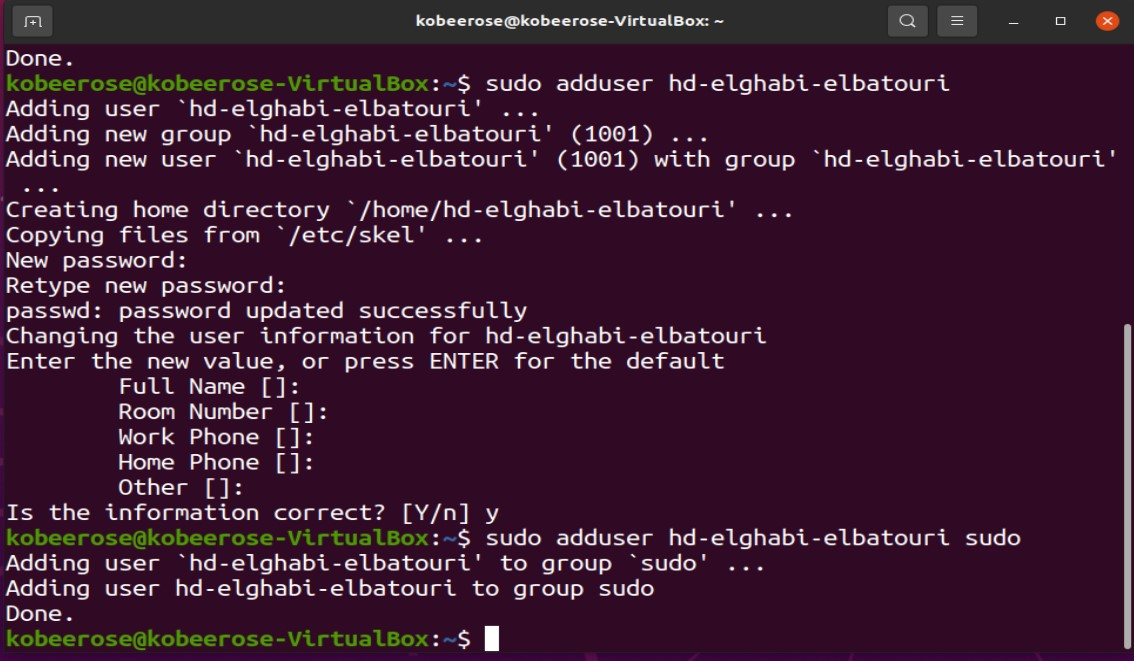
\includegraphics[width=1\linewidth]{Big_Data/Hadoop/Apache Hadoop Installation/Adding new user to sudo group}
\end{center} 
\caption{Adding new user to sudo group} 
\end{figure} 
\FloatBarrier



\par Downloadning Hadoop, Java Development Kit, code_java.zip ( the java source code of the MapReduce "word count" program ), "classpath" script used to set up the variables of the compilation environment, and finally The poeme.txt file to used for manipulations.
\\
\begin{figure}[!htb] 
\begin{center} 
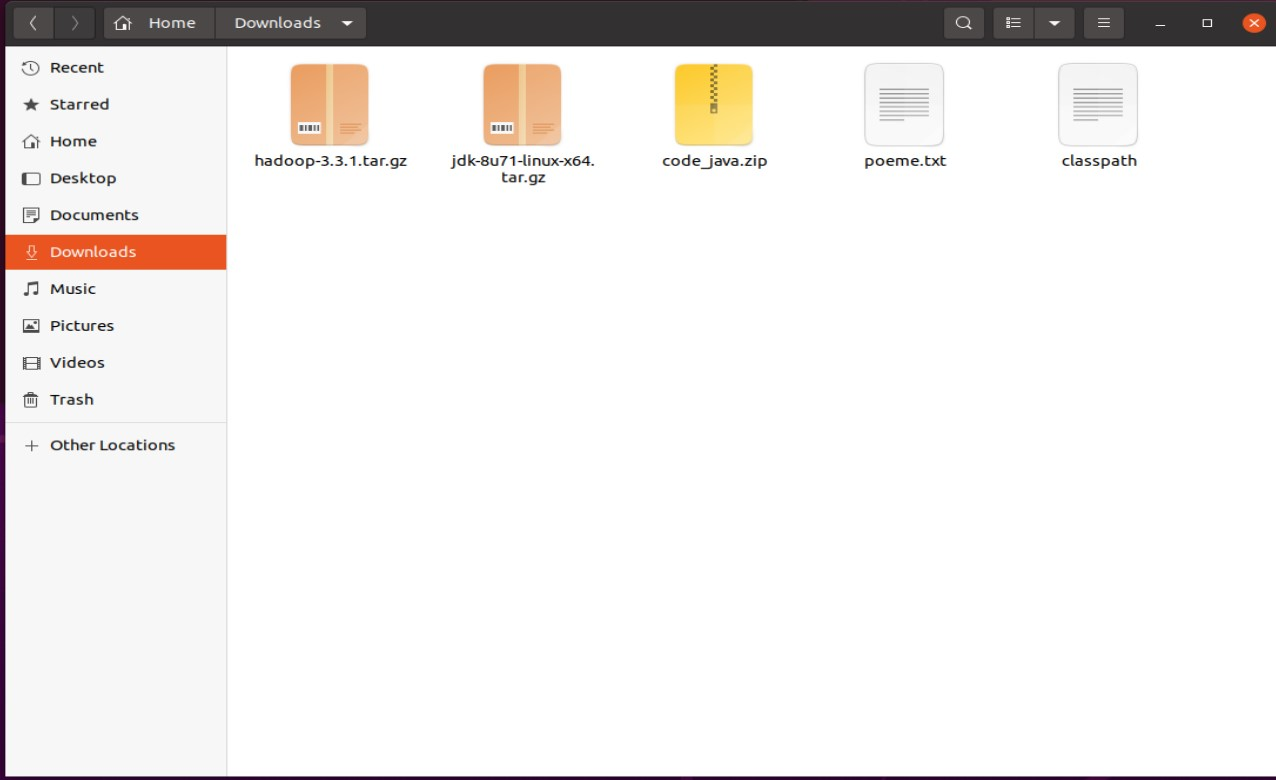
\includegraphics[width=1\linewidth]{Big_Data/Hadoop/Apache Hadoop Installation/Downloading required files} 
\end{center} 
\caption{Downloading required files} 
\end{figure} 
\FloatBarrier

\section{Setting up the ssh key }

\par Install the necessary "openssh-server" package for ssh.
\\
\begin{figure}[!htb] 
\begin{center} 
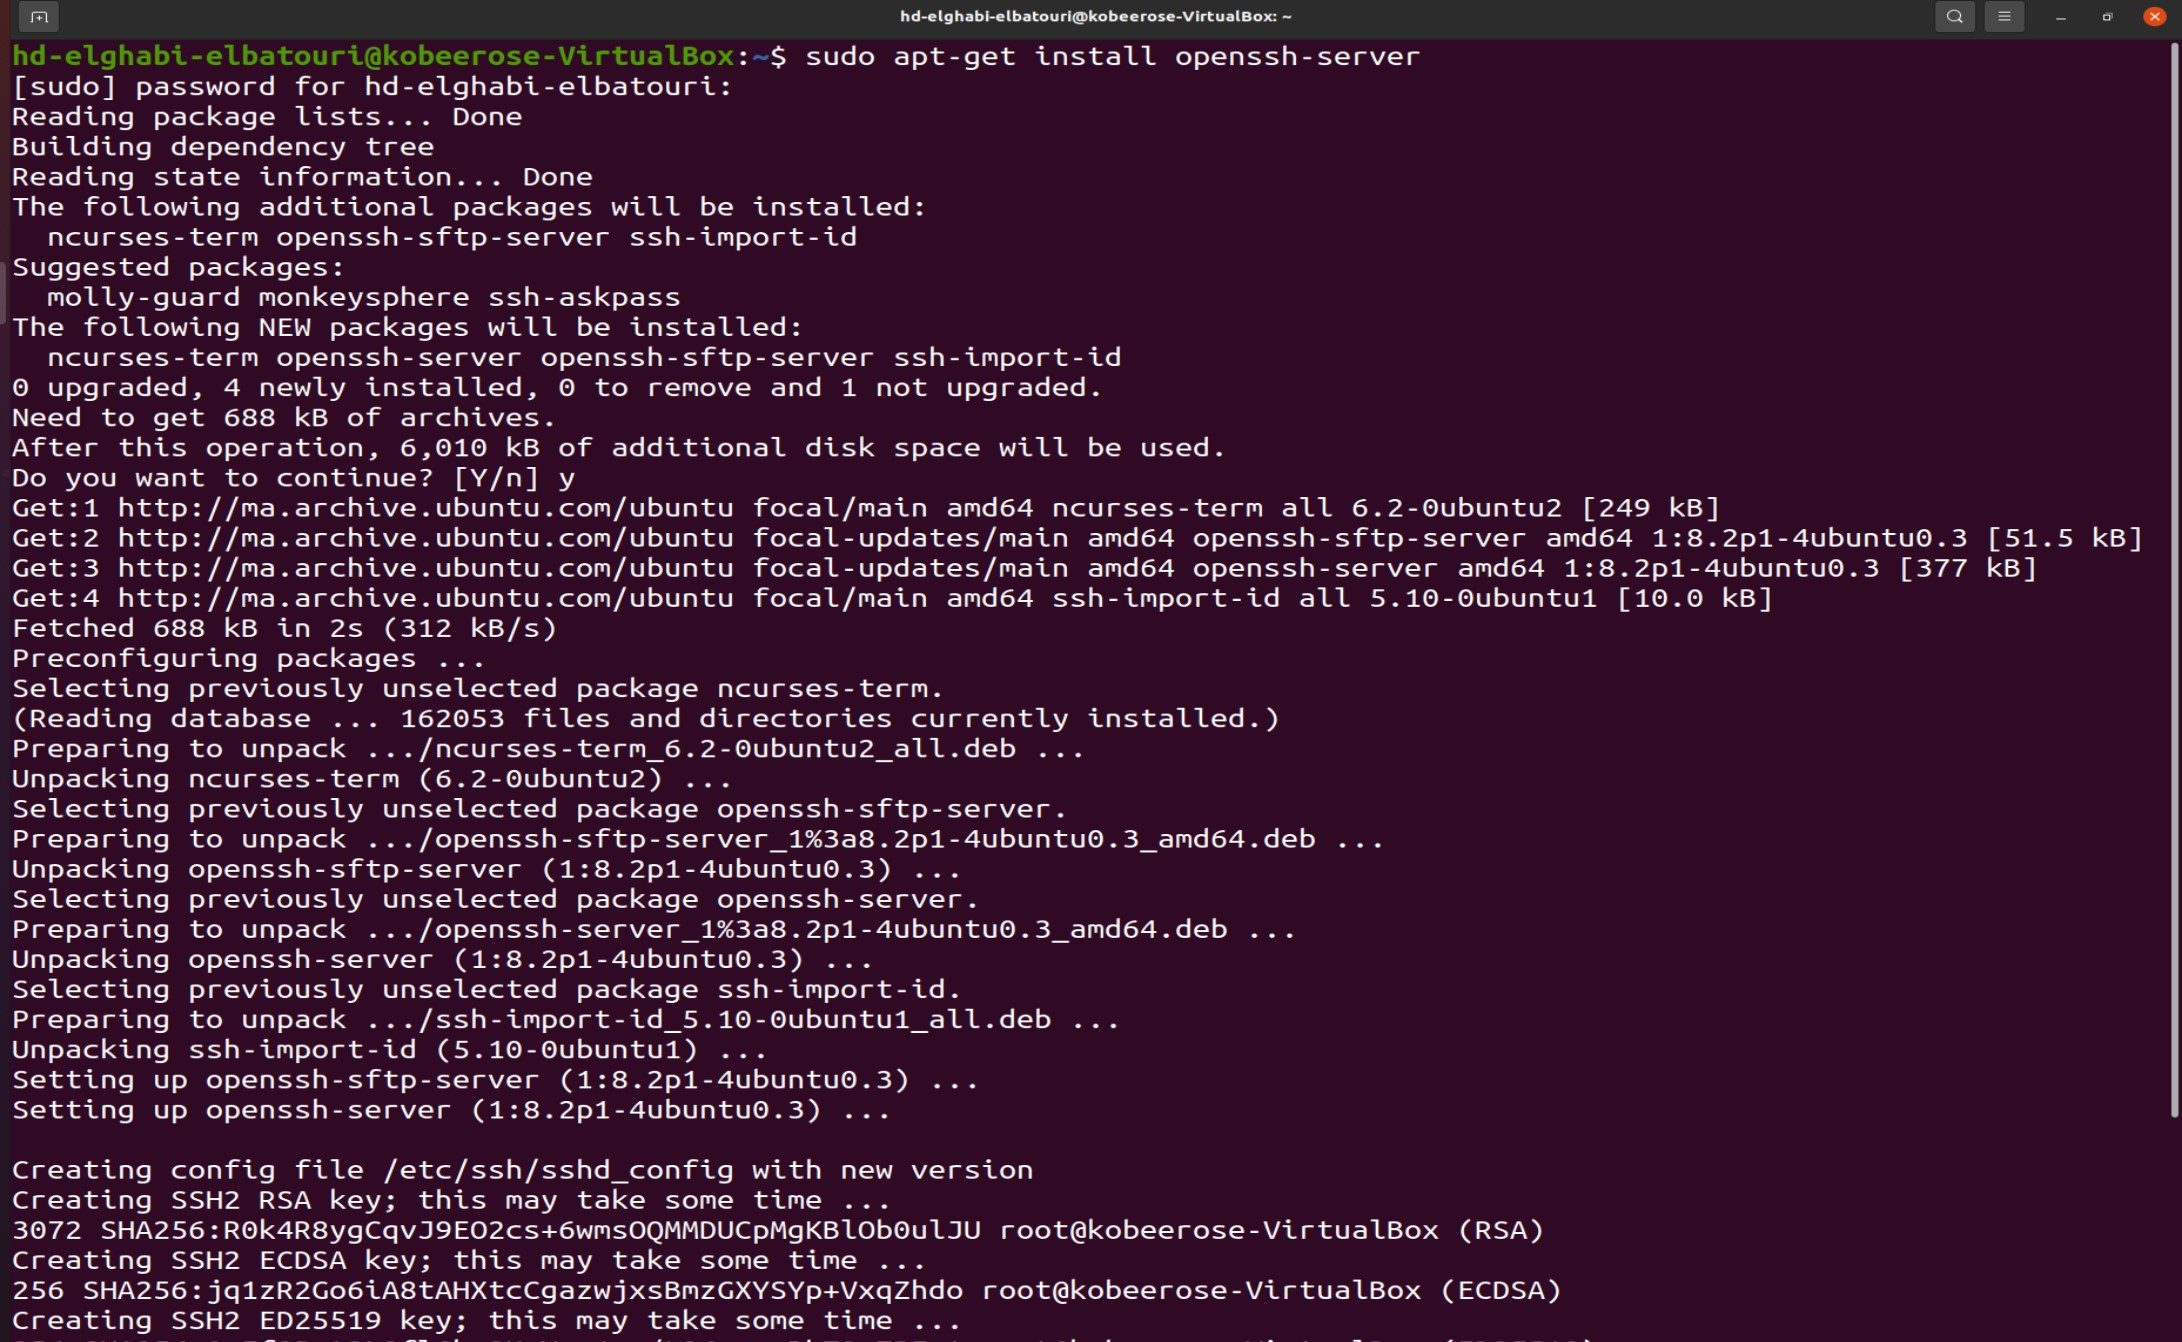
\includegraphics[width=1\linewidth]{Big_Data/Hadoop/Apache Hadoop Installation/Installing openssh-server} 
\end{center} 
\caption{Installing openssh-server} 
\end{figure} 
\FloatBarrier



\par Now you have to set up the ssh key for your own account.
\\
\begin{figure}[!htb] 
\begin{center} 
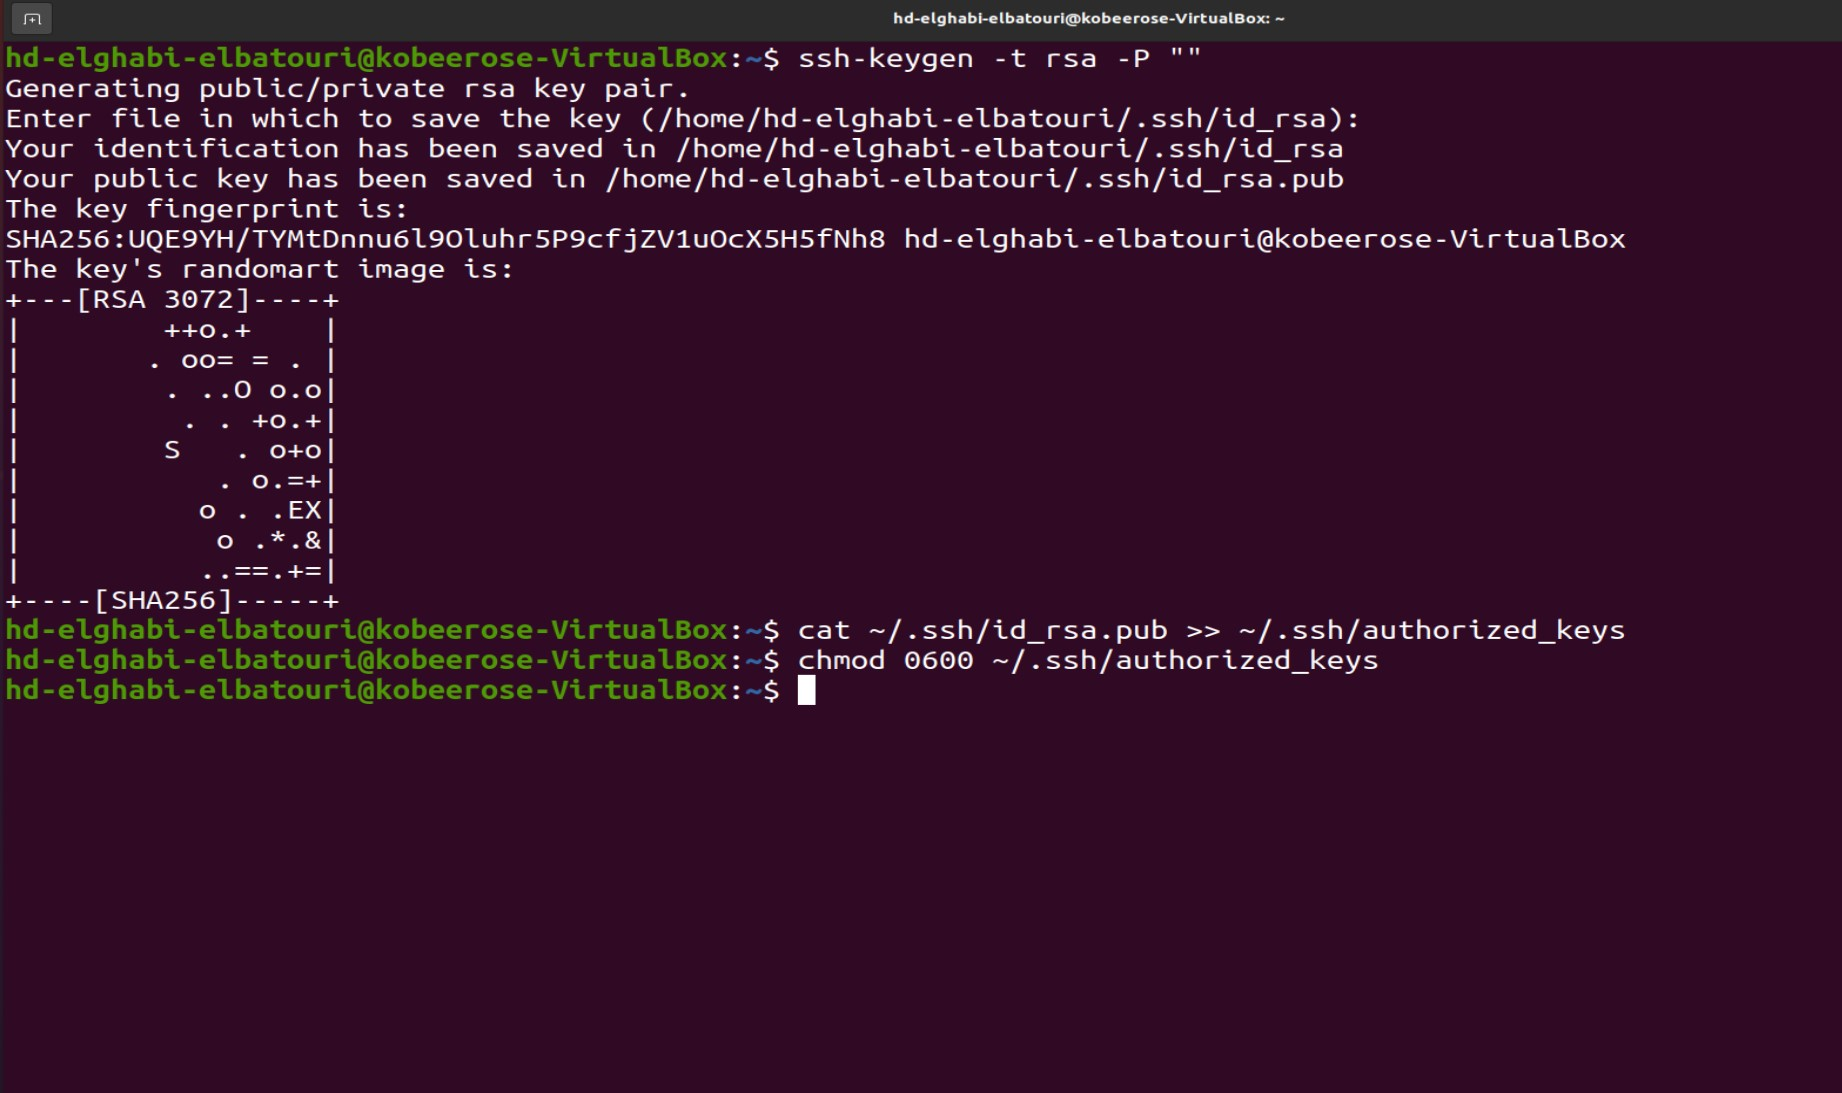
\includegraphics[width=1\linewidth]{Big_Data/Hadoop/Apache Hadoop Installation/Creating SSH key} 
\end{center} 
\caption{Creating SSH key} 
\end{figure} 
\FloatBarrier

\section{Section_name}

\par we Copy the public key to the localhost server.
\\
\begin{figure}[!htb] 
\begin{center} 
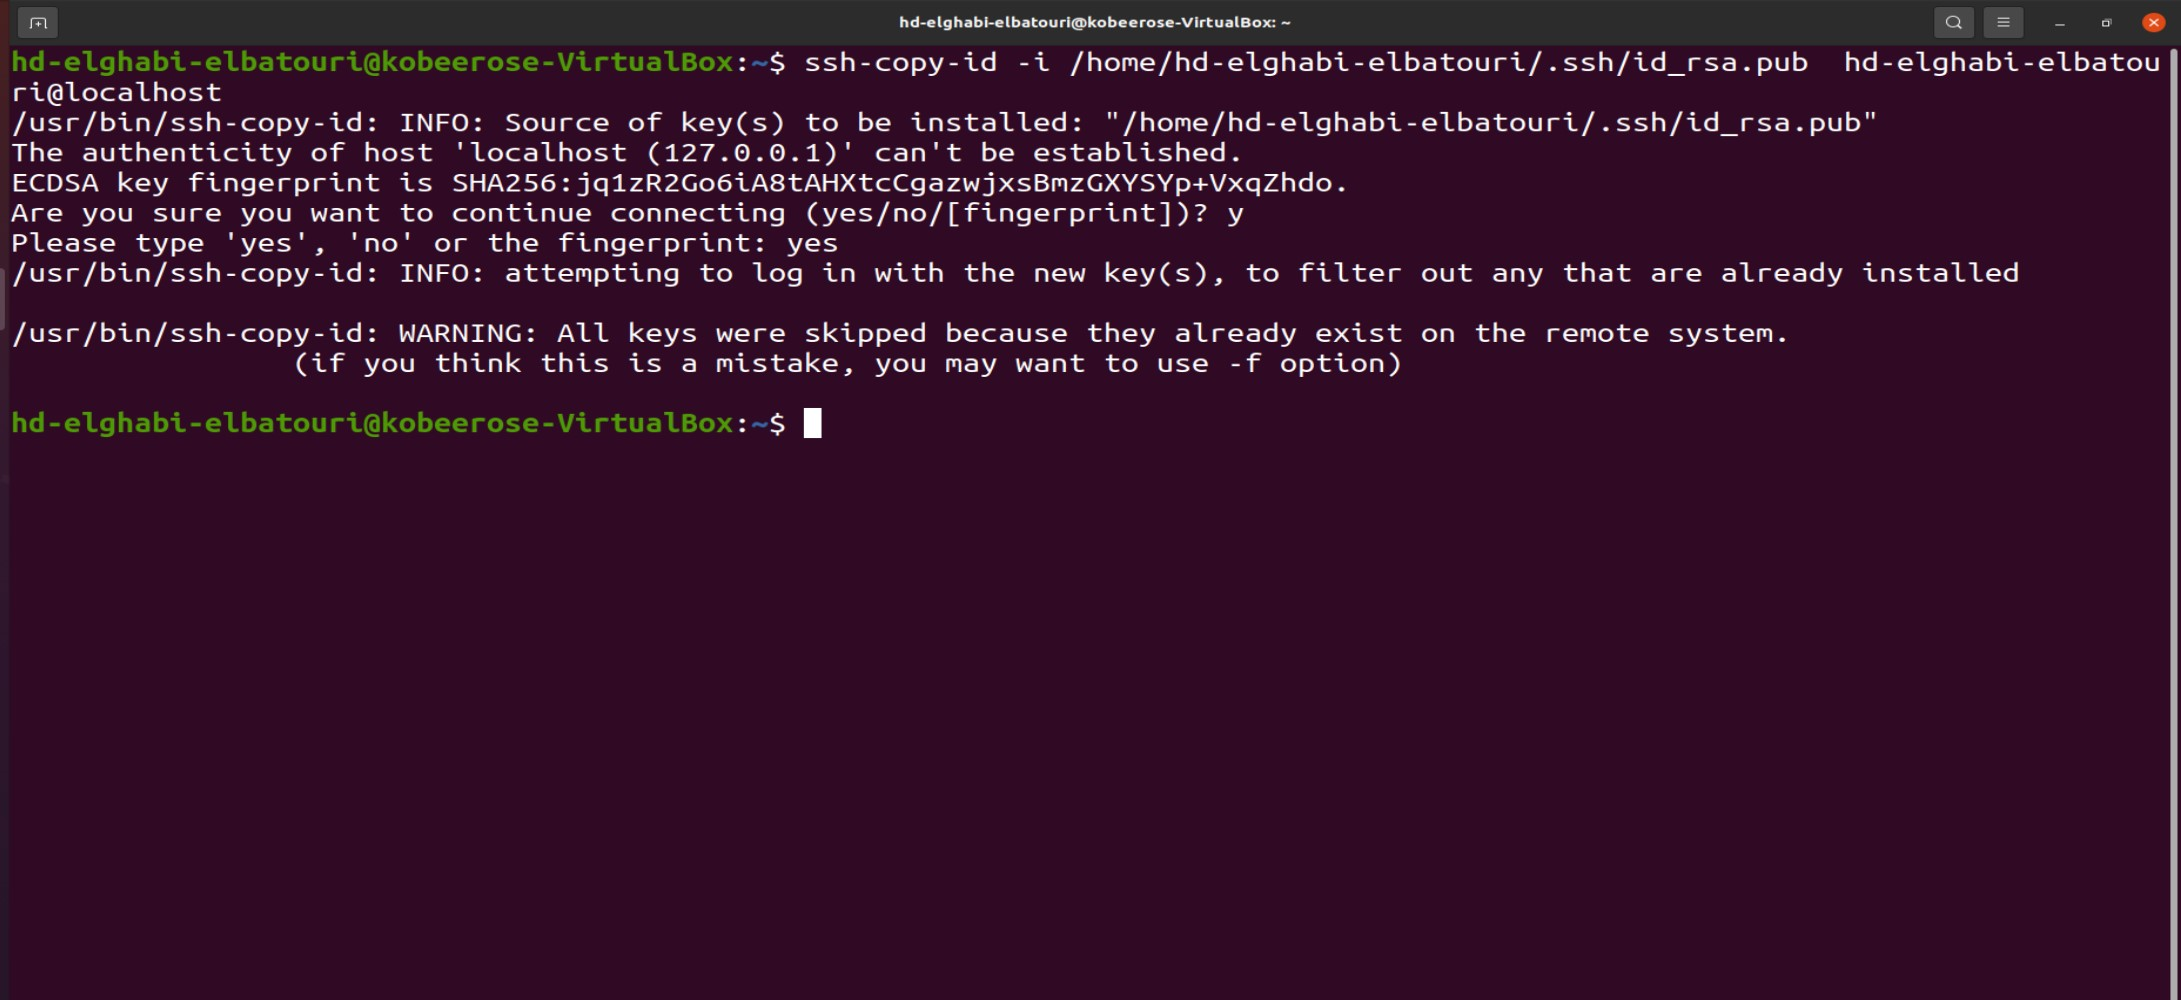
\includegraphics[width=1\linewidth]{Big_Data/Hadoop/Apache Hadoop Installation/Copying the key} 
\end{center} 
\caption{Copying the key} 
\end{figure} 
\FloatBarrier



\par Let's test the connection to localhost.
\\
\begin{figure}[!htb] 
\begin{center} 
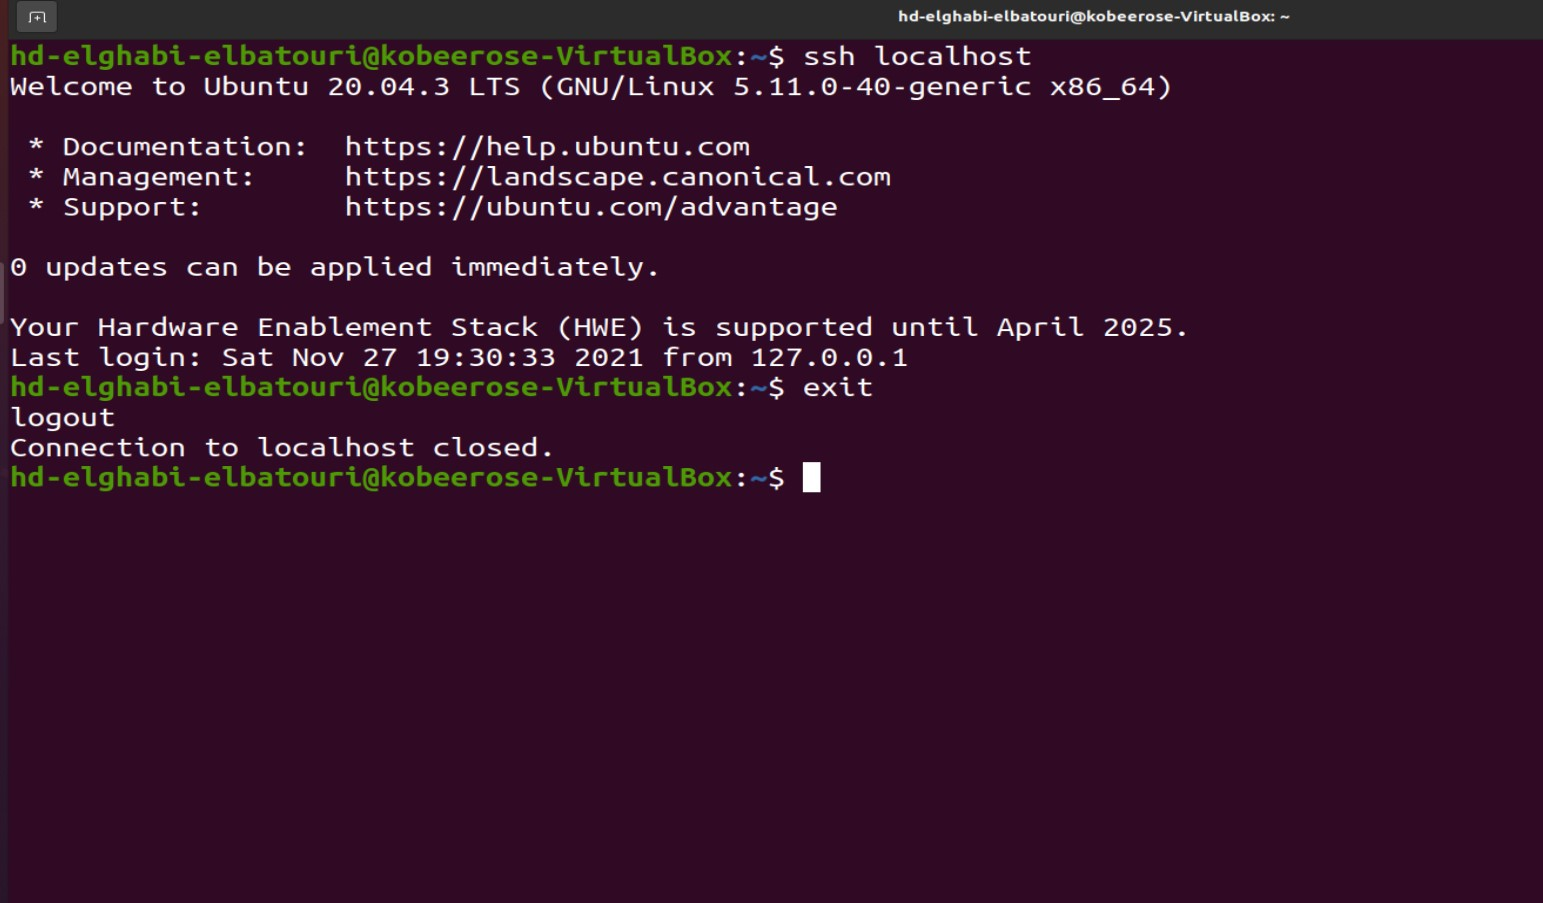
\includegraphics[width=1\linewidth]{Big_Data/Hadoop/Apache Hadoop Installation/Connecting to localhost} 
\end{center} 
\caption{Connecting to localhost} 
\end{figure} 
\FloatBarrier

\section{Installing JAVA 8}

\par We will install in the / opt / java directory to ensure a global access.
\\
\begin{figure}[!htb] 
\begin{center} 
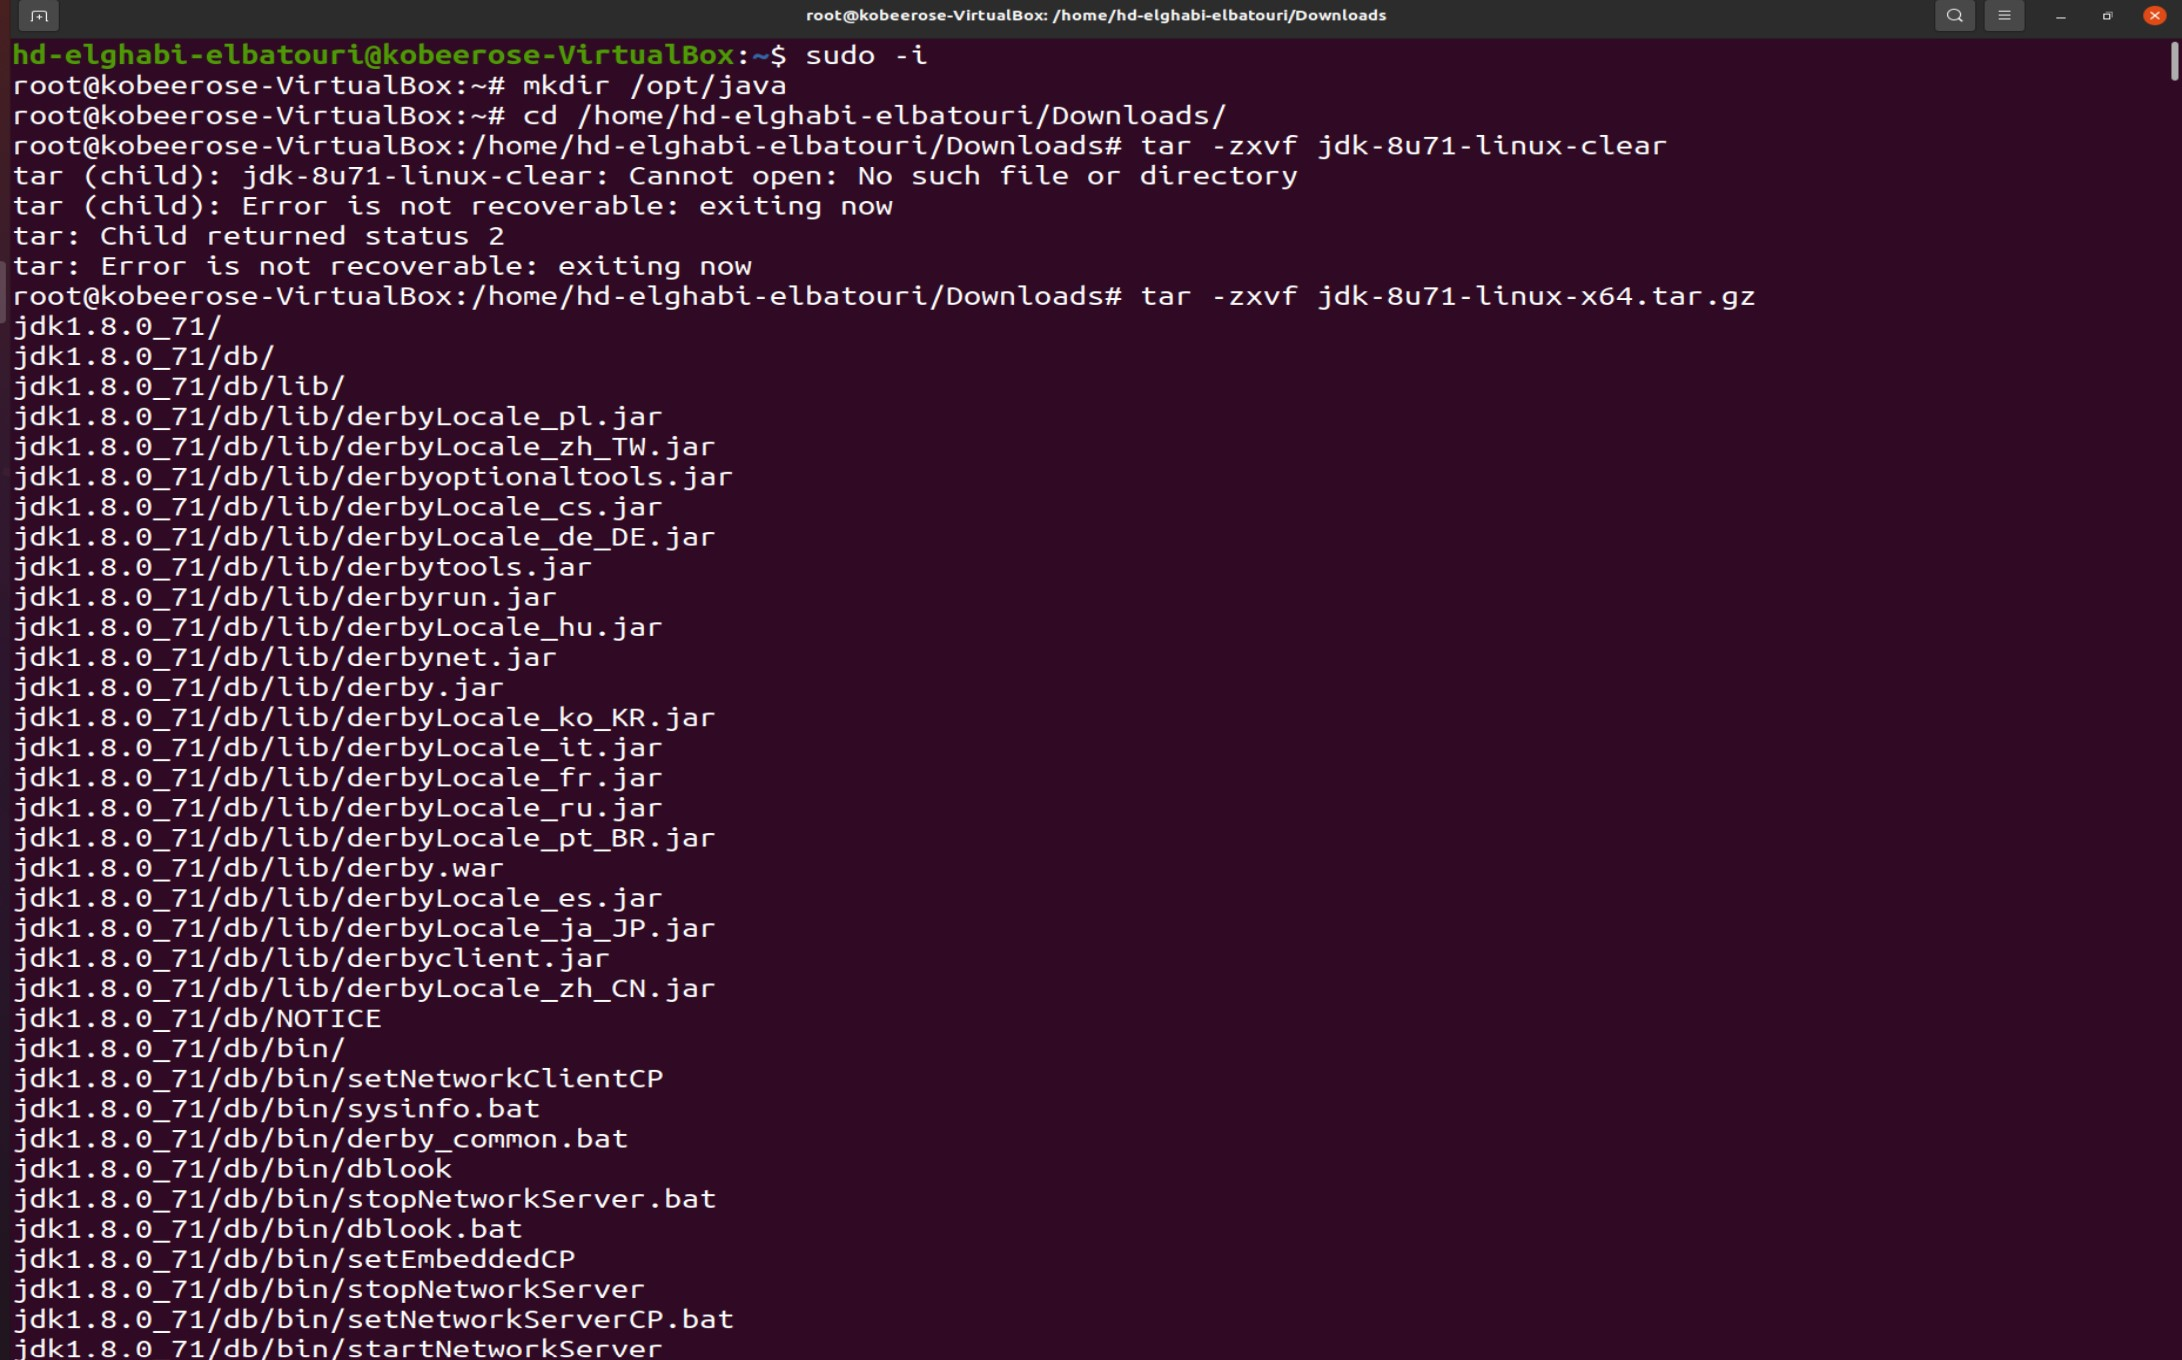
\includegraphics[width=1\linewidth]{Big_Data/Hadoop/Apache Hadoop Installation/Extracting files} 
\end{center} 
\caption{Extracting files} 
\end{figure} 
\FloatBarrier

\begin{figure}[!htb] 
\begin{center} 
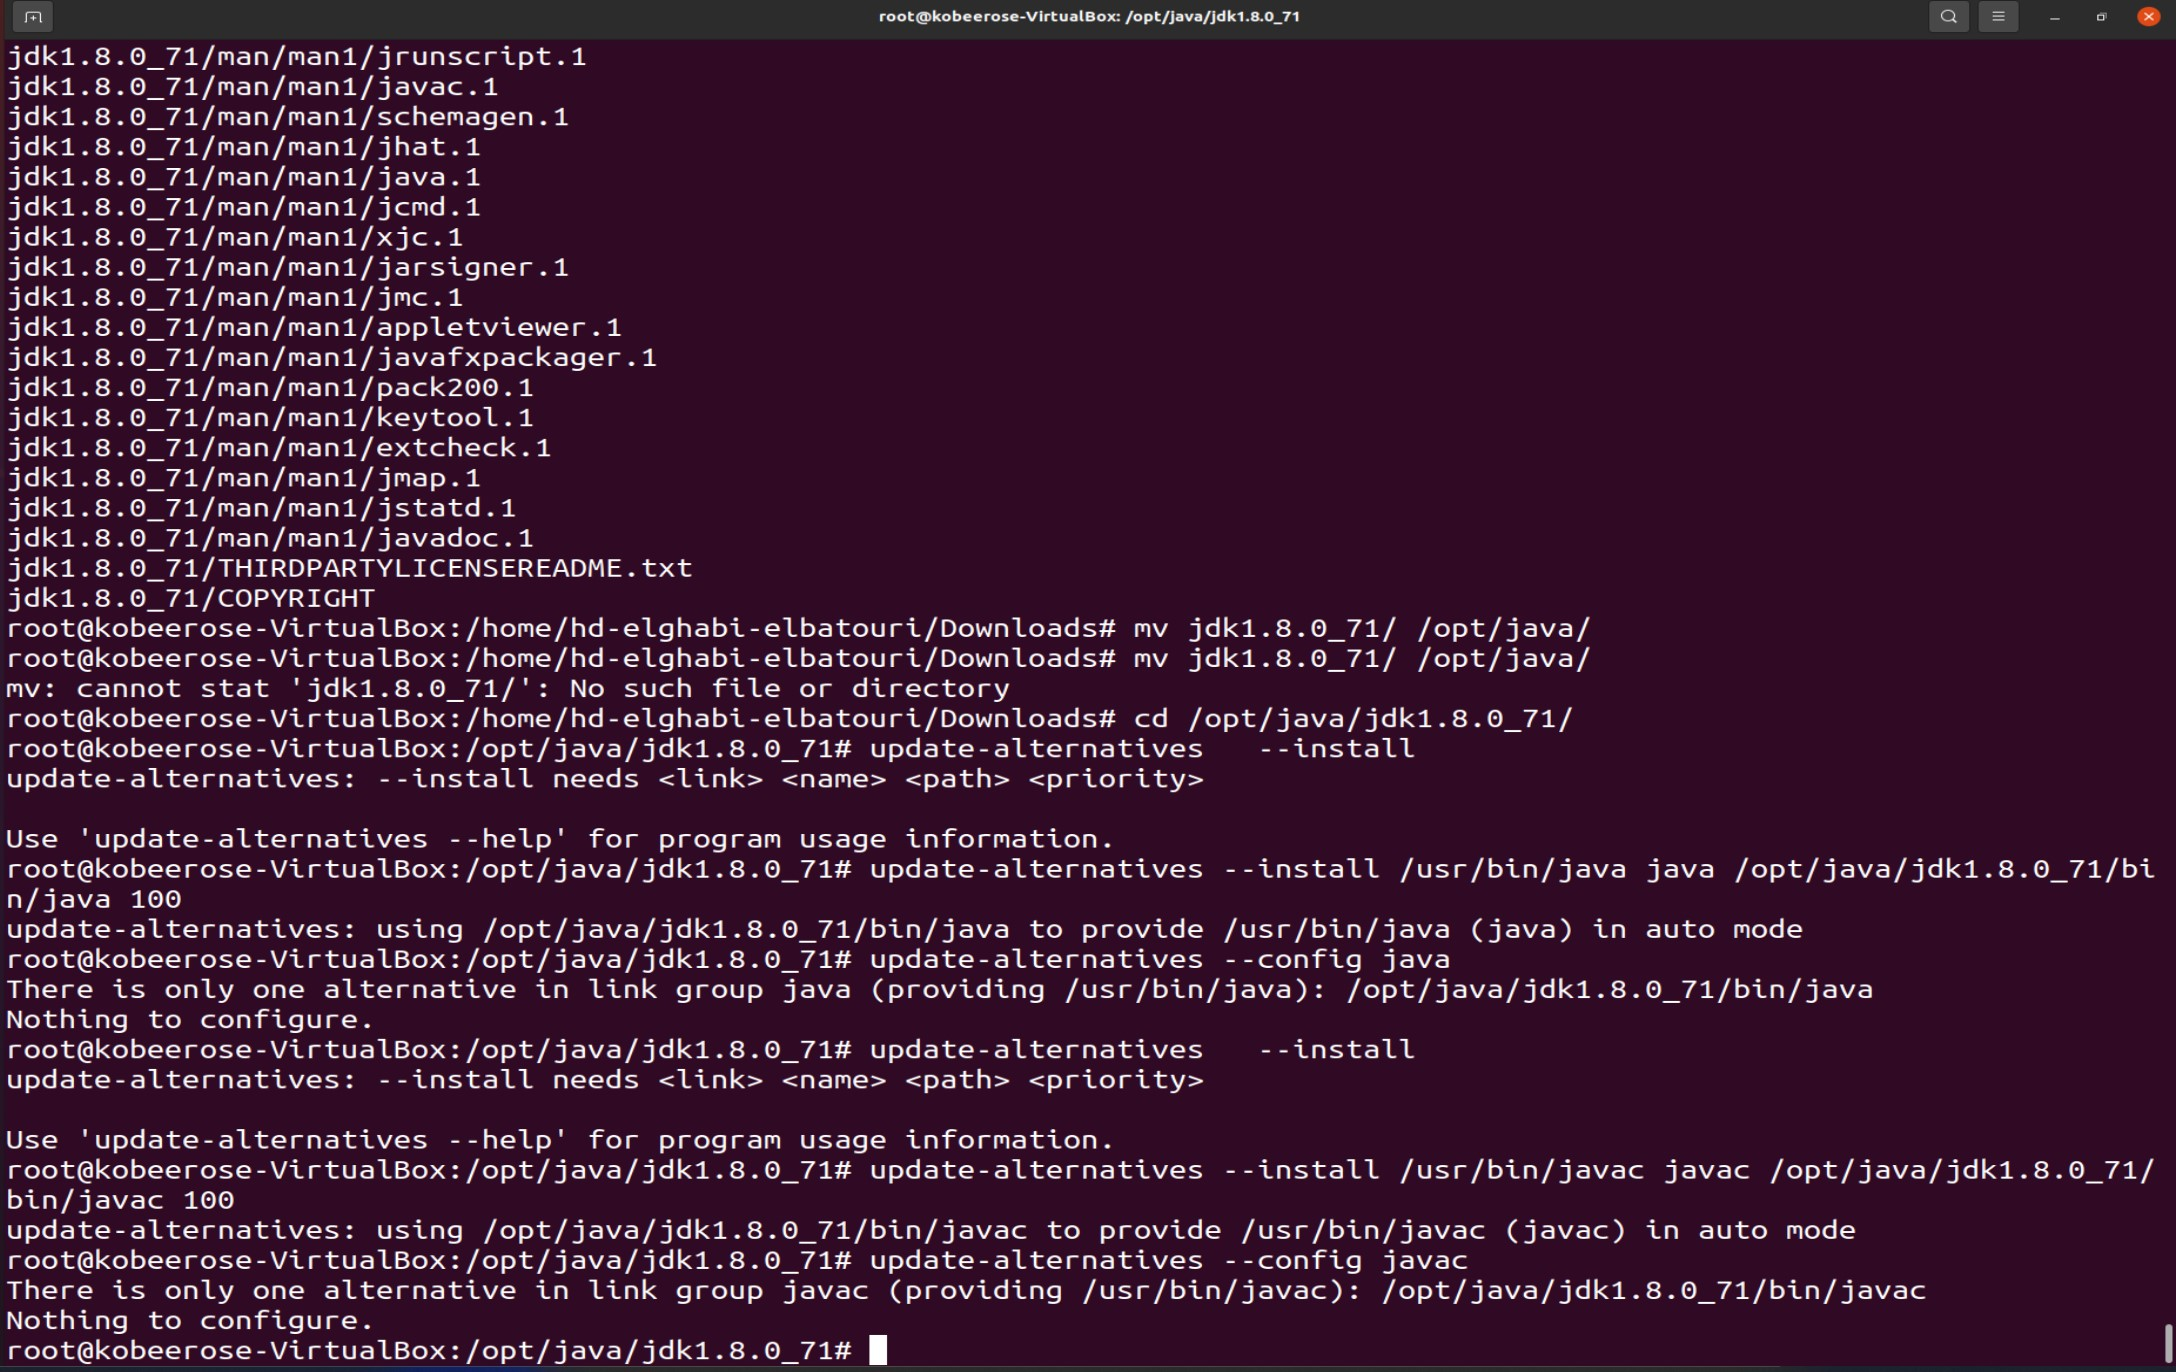
\includegraphics[width=1\linewidth]{Big_Data/Hadoop/Apache Hadoop Installation/Installing java and javac} 
\end{center} 
\caption{Installing java and javac} 
\end{figure} 
\FloatBarrier


\par To permanently set up JAVA environment variables for all users, we will configure profile file.
\\
\begin{figure}[!htb] 
\begin{center} 
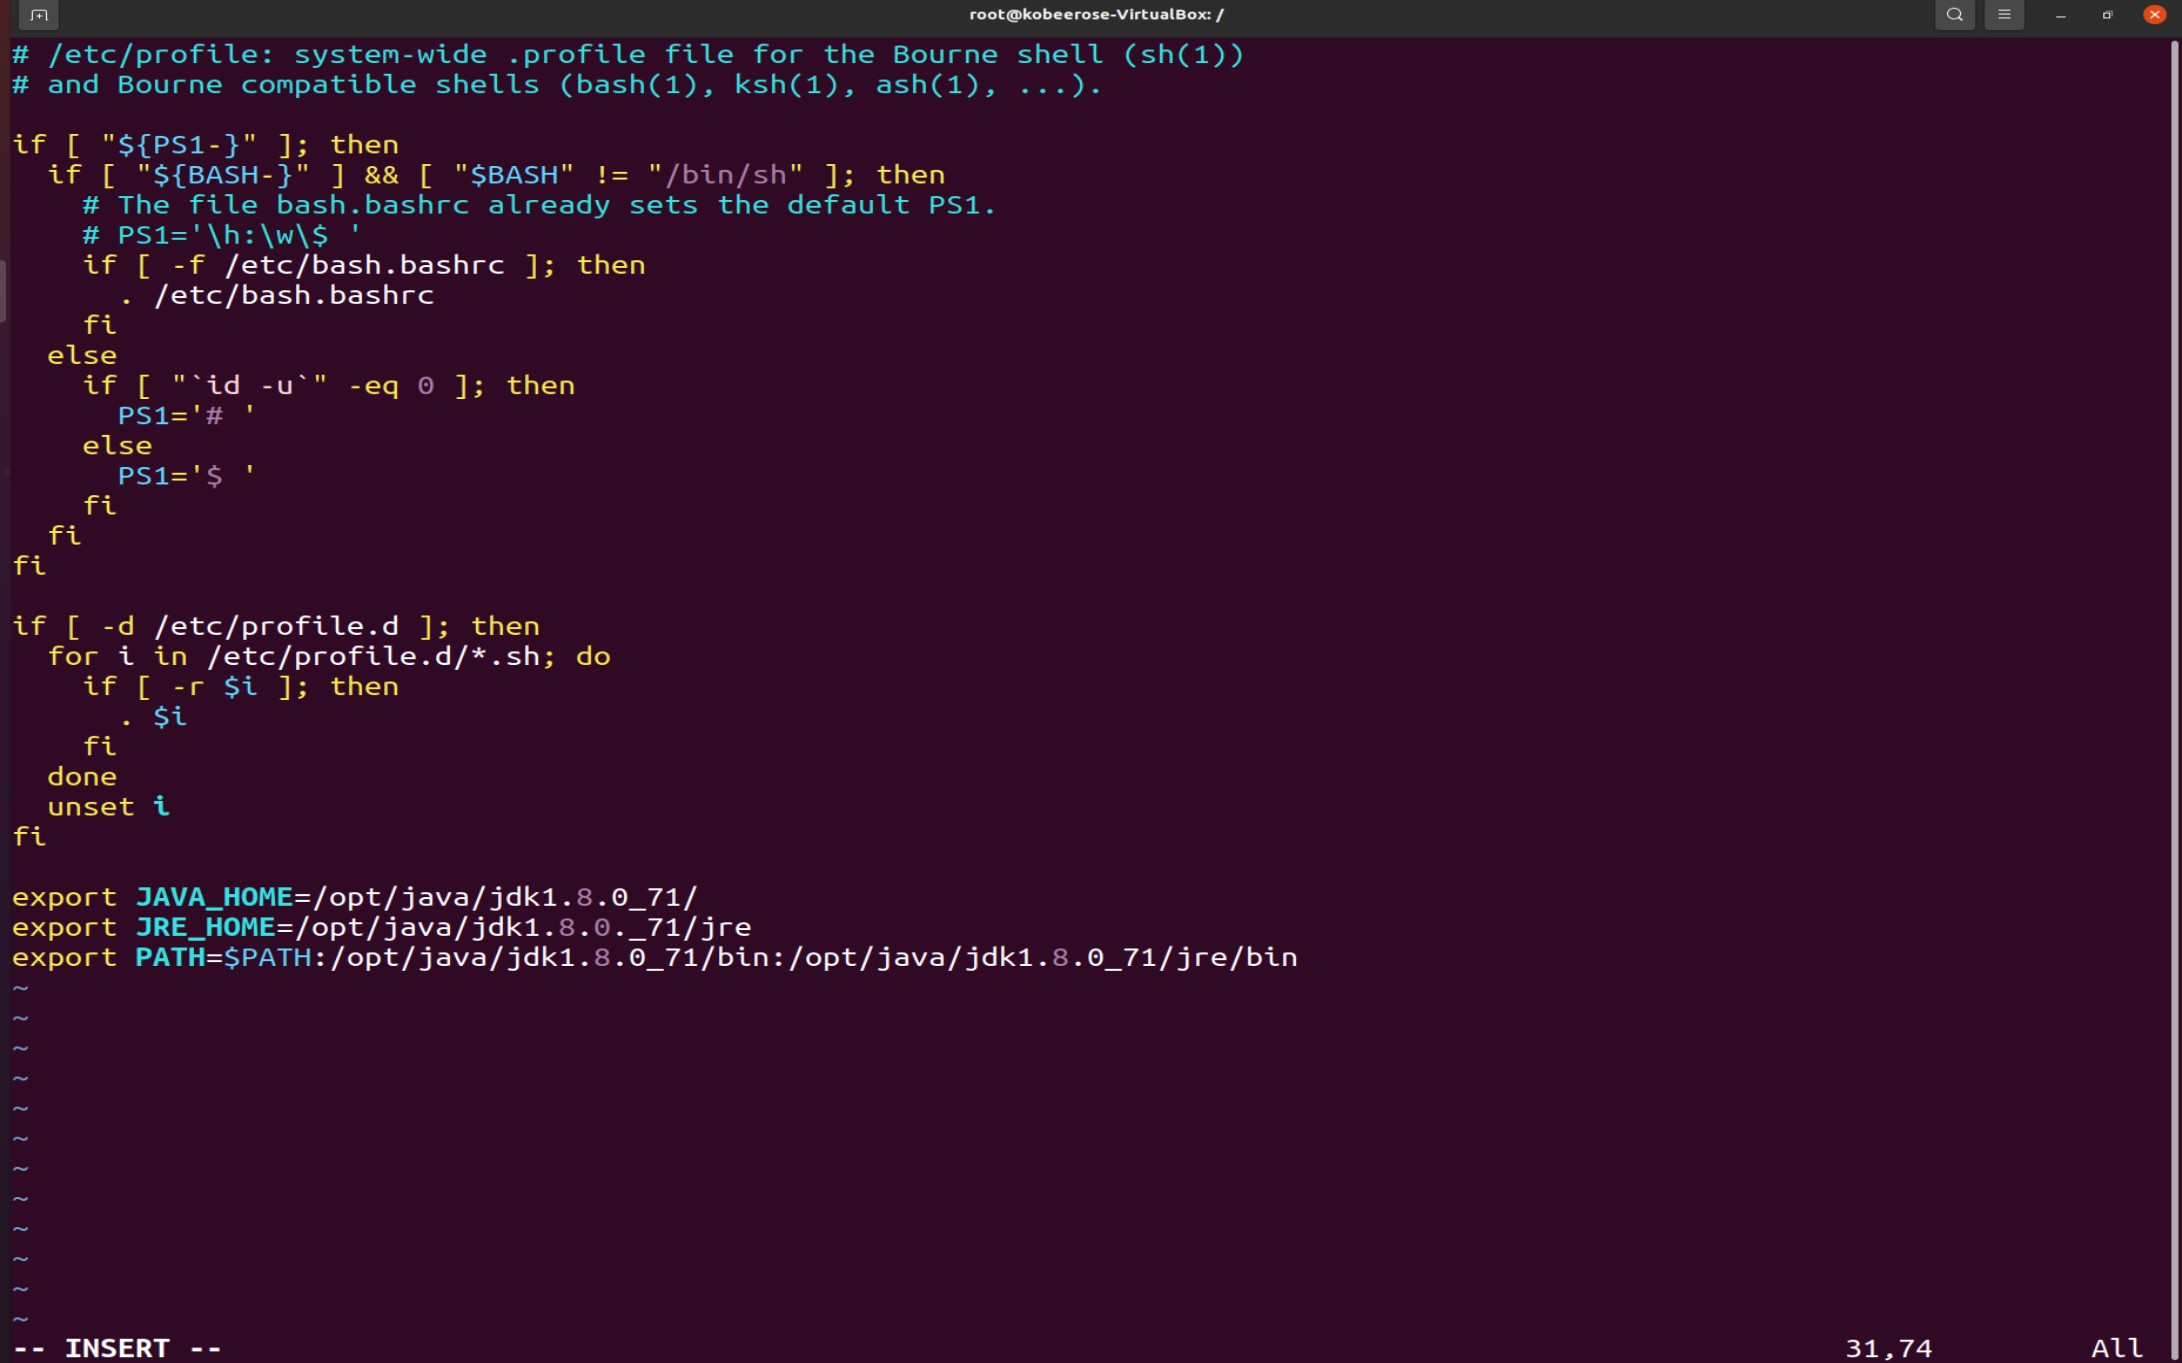
\includegraphics[width=1\linewidth]{Big_Data/Hadoop/Apache Hadoop Installation/profile file config} 
\end{center} 
\caption{profile file config} 
\end{figure} 
\FloatBarrier

\par Le'ts can test the setting of environment variables in the hadoop terminal.
\\
\begin{figure}[!htb] 
\begin{center} 
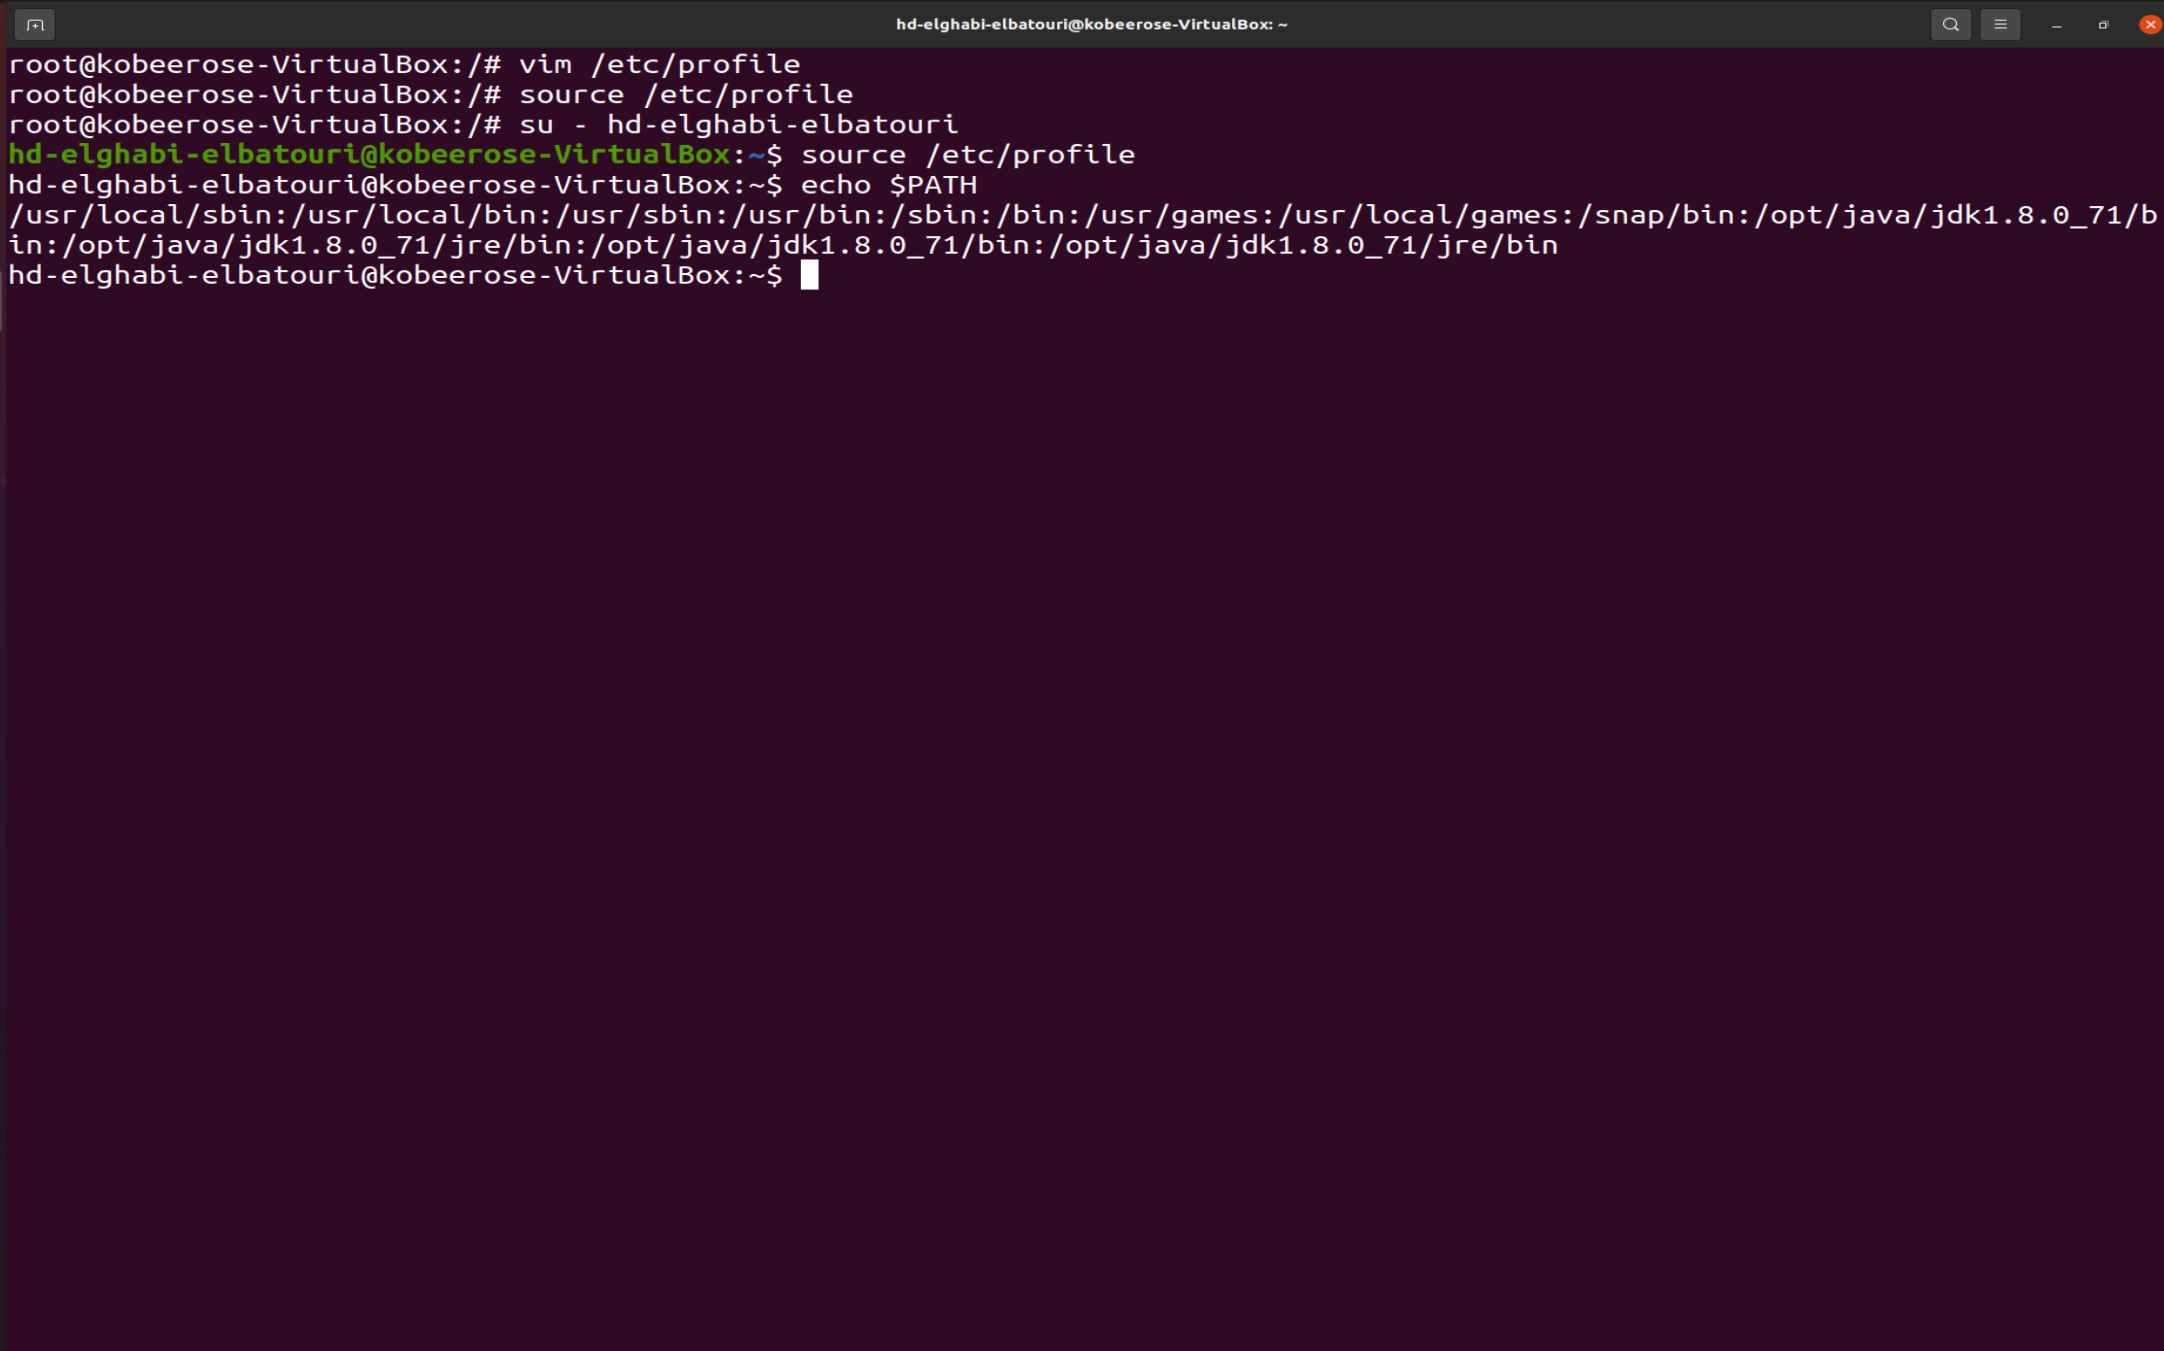
\includegraphics[width=1\linewidth]{Big_Data/Hadoop/Apache Hadoop Installation/Verifying PATH} 
\end{center} 
\caption{Verifying PATH} 
\end{figure} 
\FloatBarrier

\section{Installing Apache Hadoop 3.3.1}

\par Extracting files and Installing Apache Hadoop.
\\
\begin{figure}[!htb] 
\begin{center} 
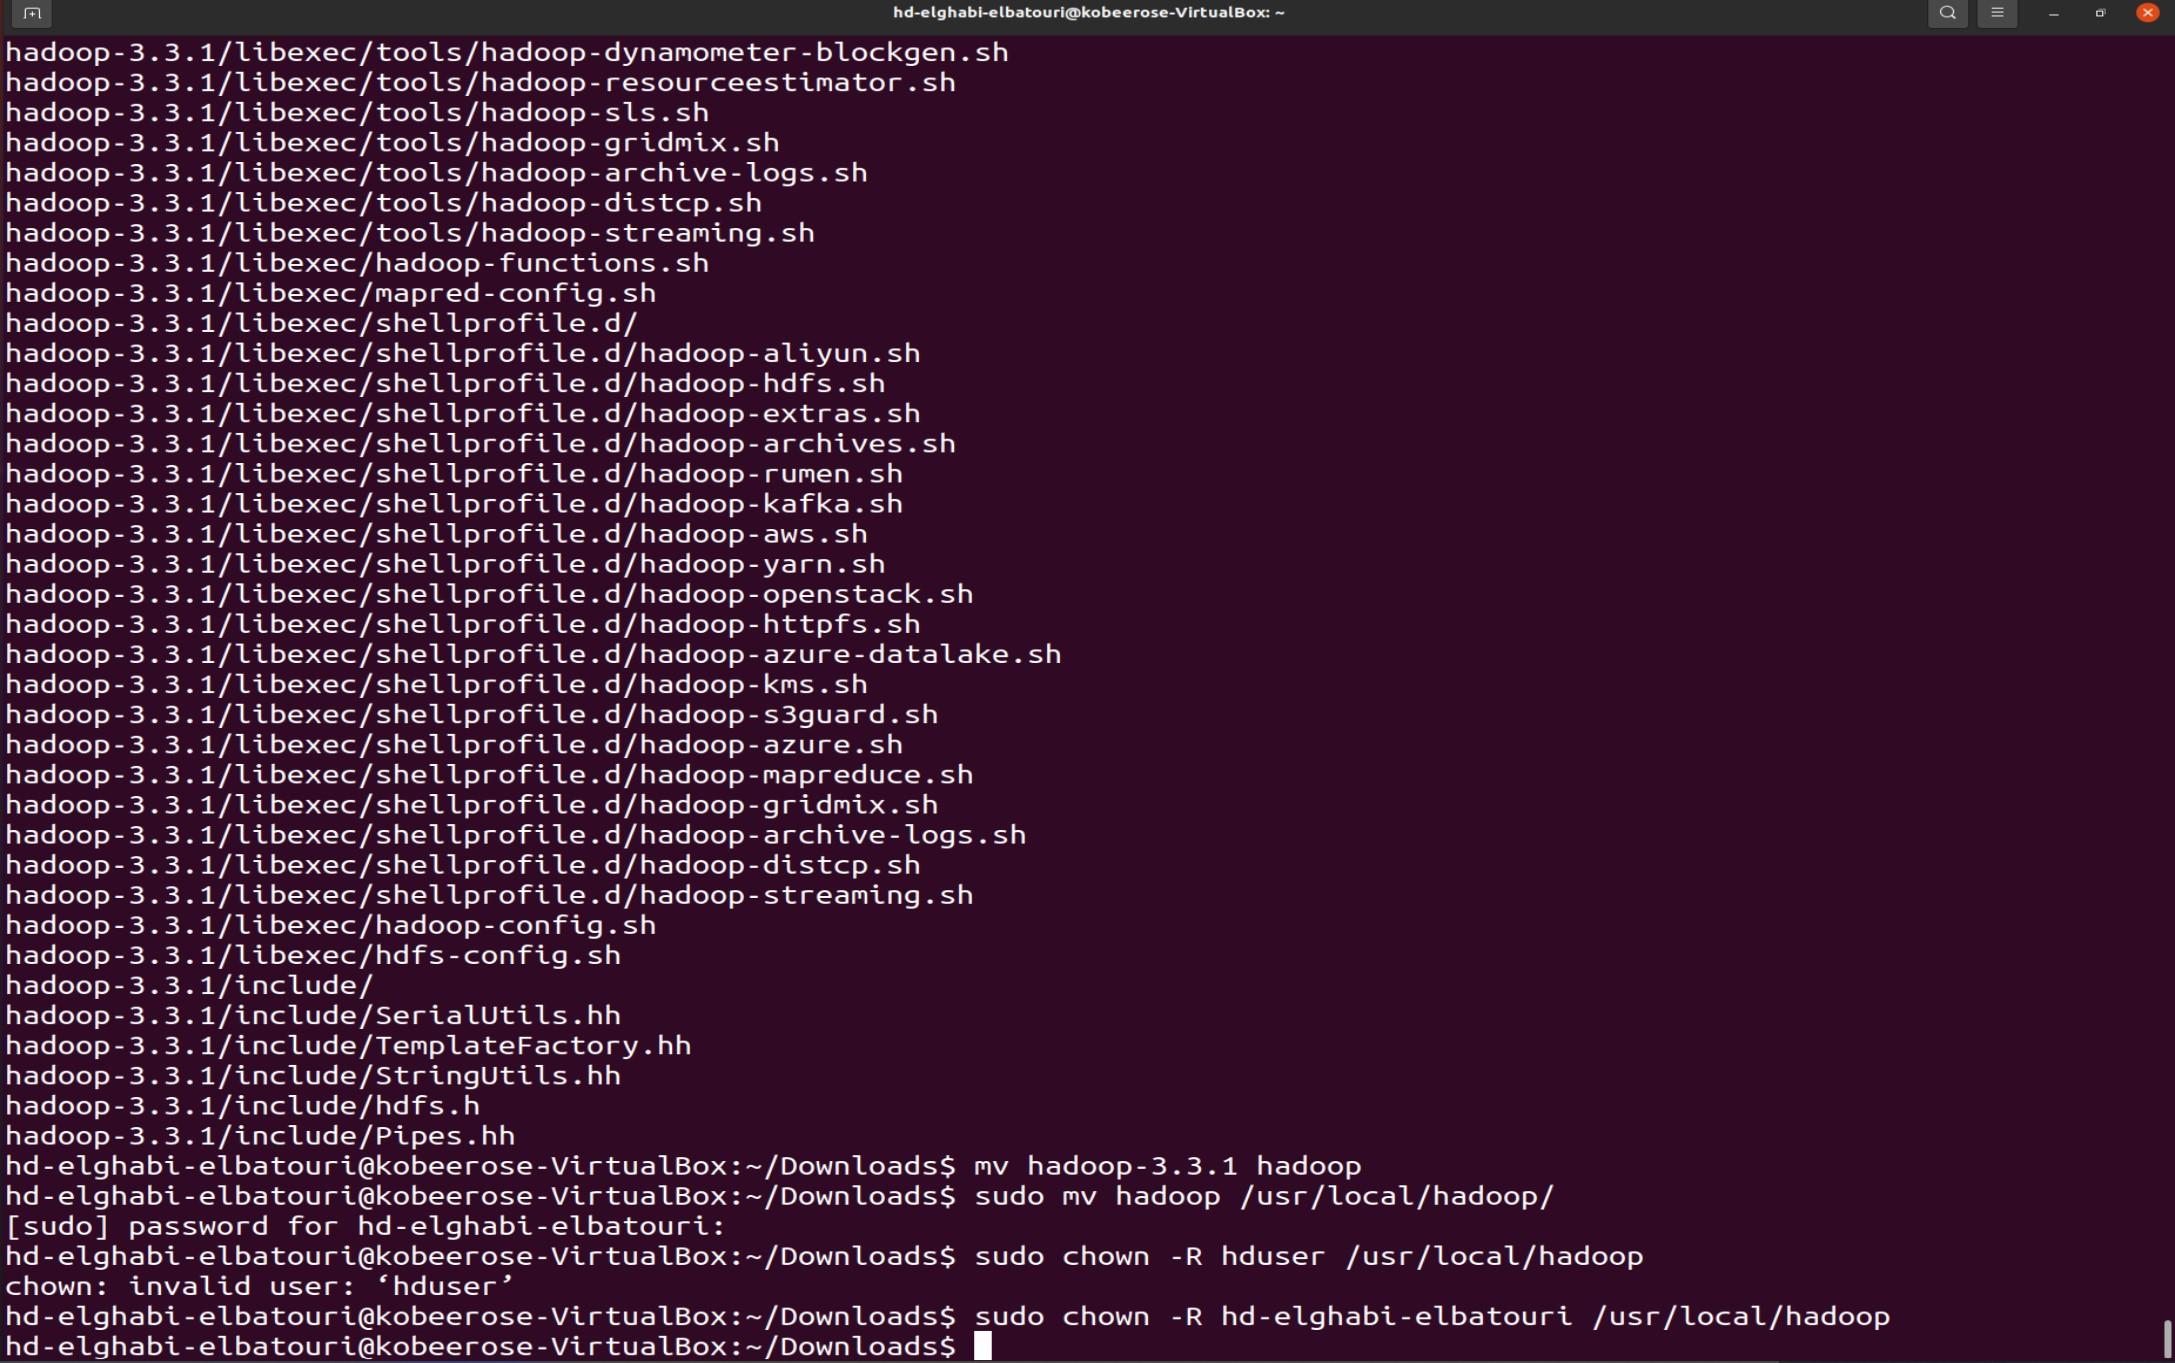
\includegraphics[width=1\linewidth]{Big_Data/Hadoop/Apache Hadoop Installation/Extracting Hadoop}
\end{center} 
\caption{Extracting Hadoop} 
\end{figure} 
\FloatBarrier


\par Create the hadoop data storage directories.
\\
\begin{figure}[!htb] 
\begin{center} 
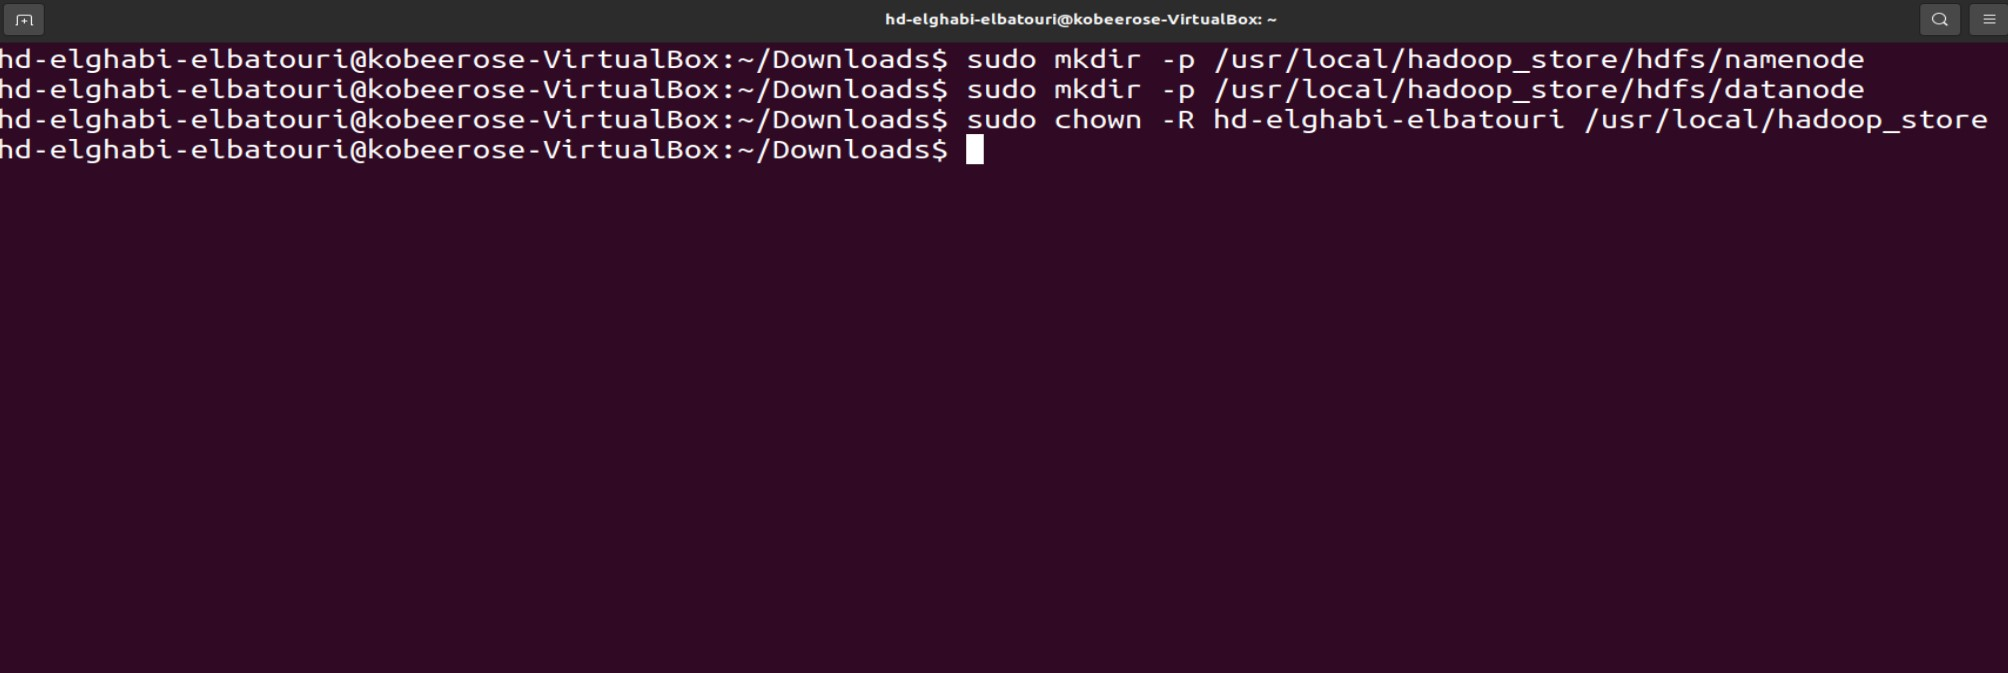
\includegraphics[width=1\linewidth]{Big_Data/Hadoop/Apache Hadoop Installation/Creating Storage repo} 
\end{center} 
\caption{Creating Storage repo} 
\end{figure} 
\FloatBarrier

\section{Configuring Apache Hadoop 3.3.1 }

\par Setting up environment variables for Hadoop.
\\
\begin{figure}[!htb] 
\begin{center} 
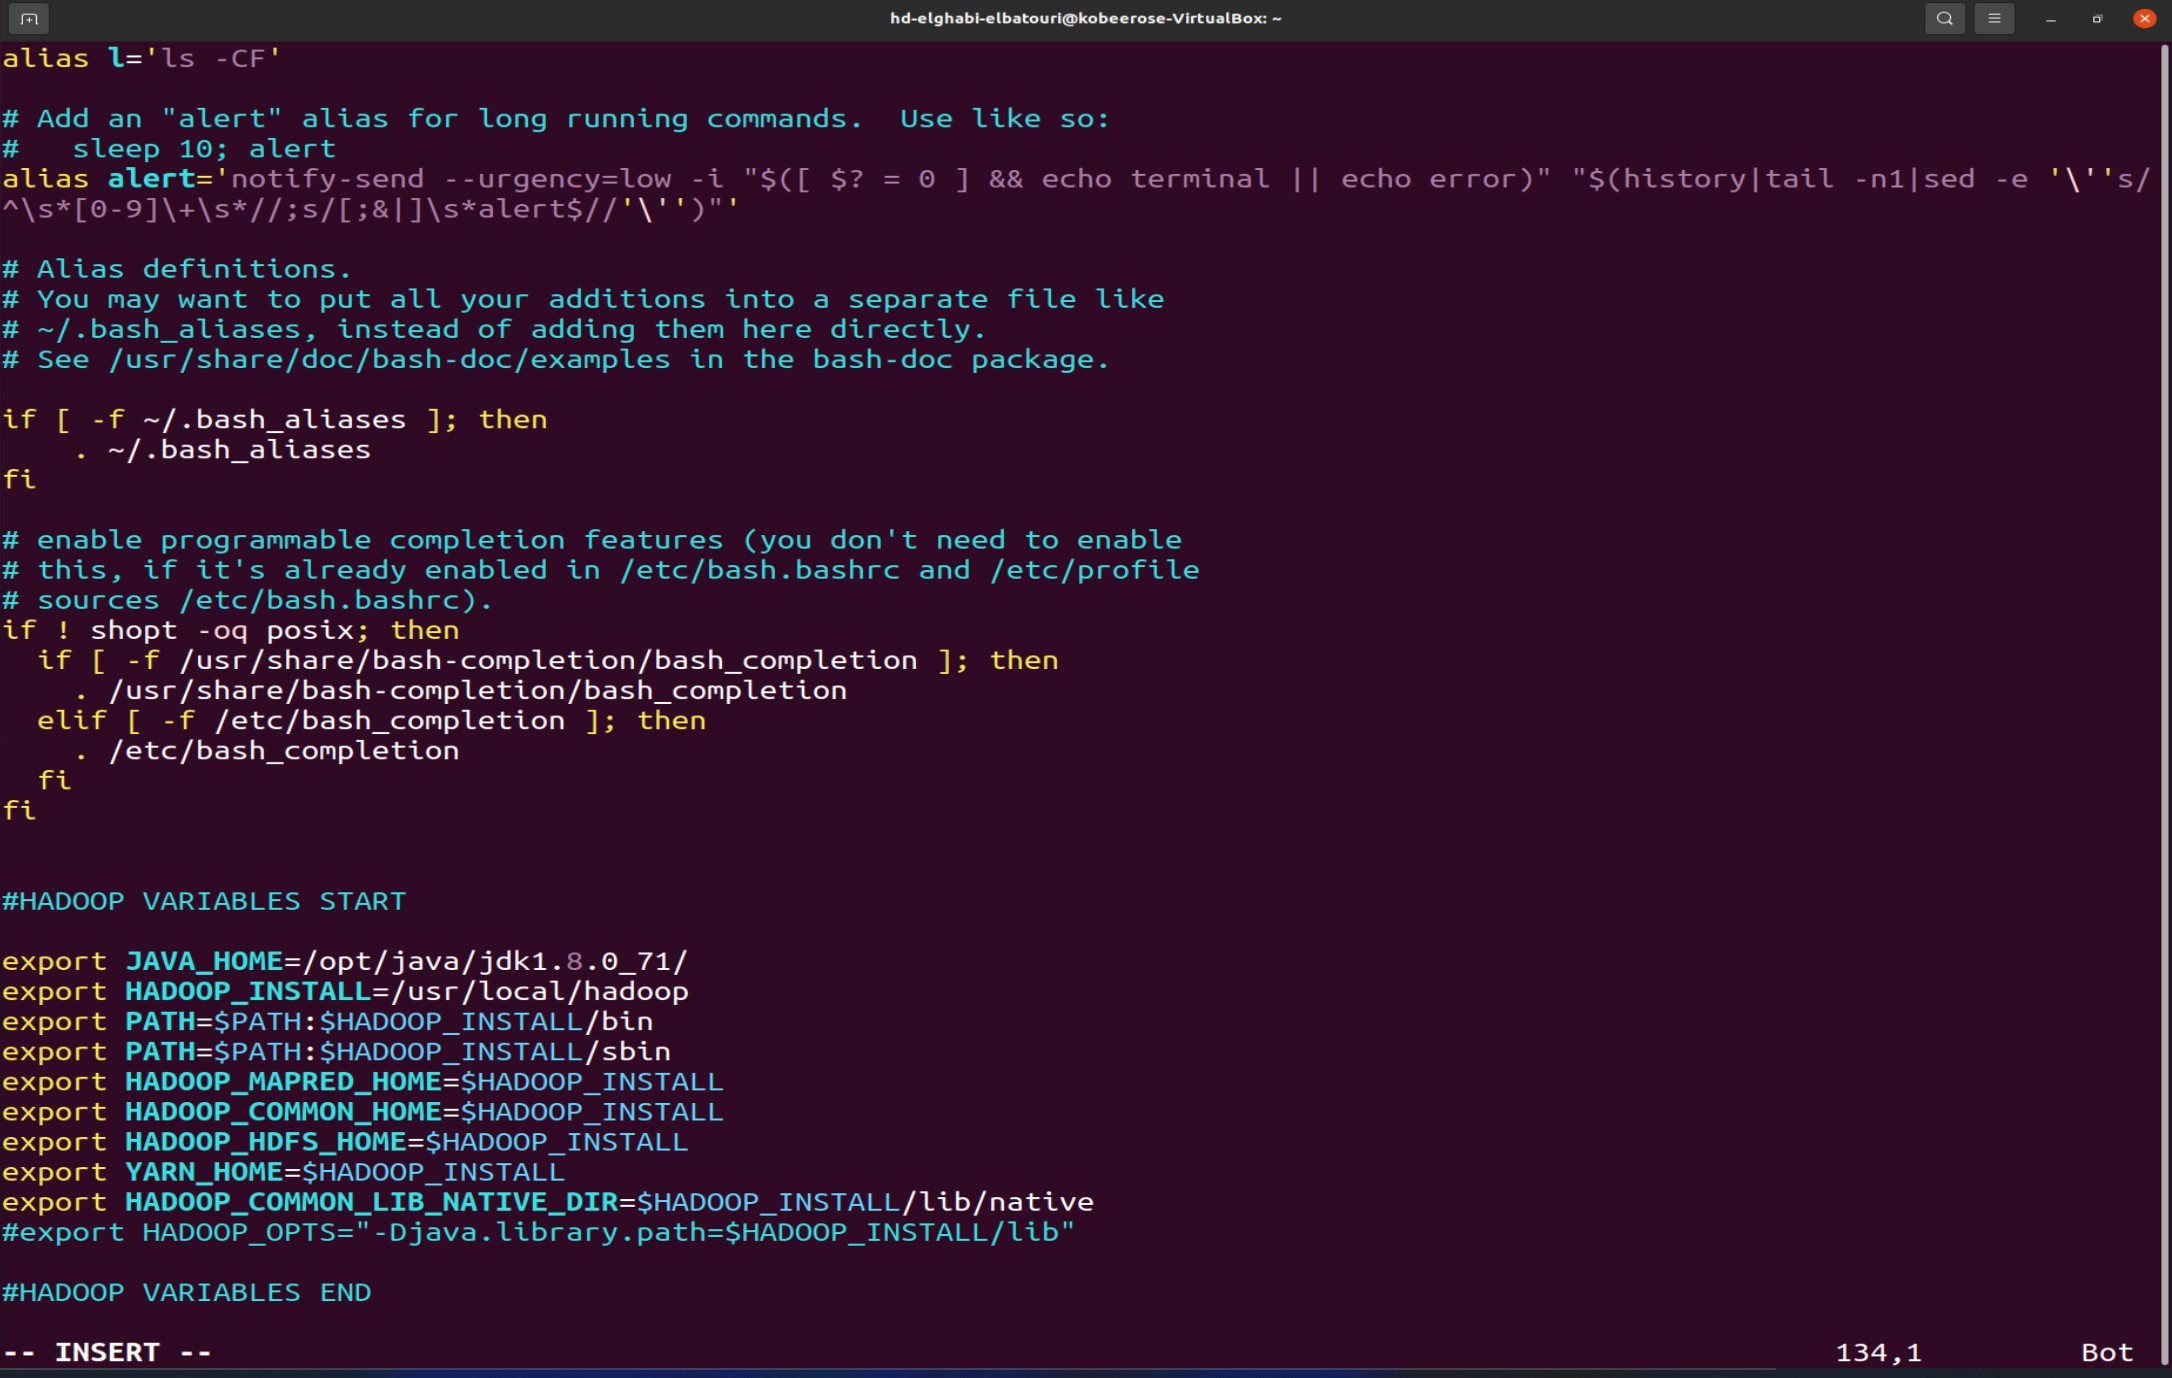
\includegraphics[width=1\linewidth]{Big_Data/Hadoop/Apache Hadoop Installation/Modifying .bashrc file} 
\end{center} 
\caption{Modifying .bashrc file} 
\end{figure} 
\FloatBarrier

\par Editing Hadoop Configuration Files: core-site.xml, hdfs-site.xml, mapred-site.xml, yarn-site.xml then Formatting of the Namenode. 
\\
\begin{figure}[!htb] 
\begin{center} 
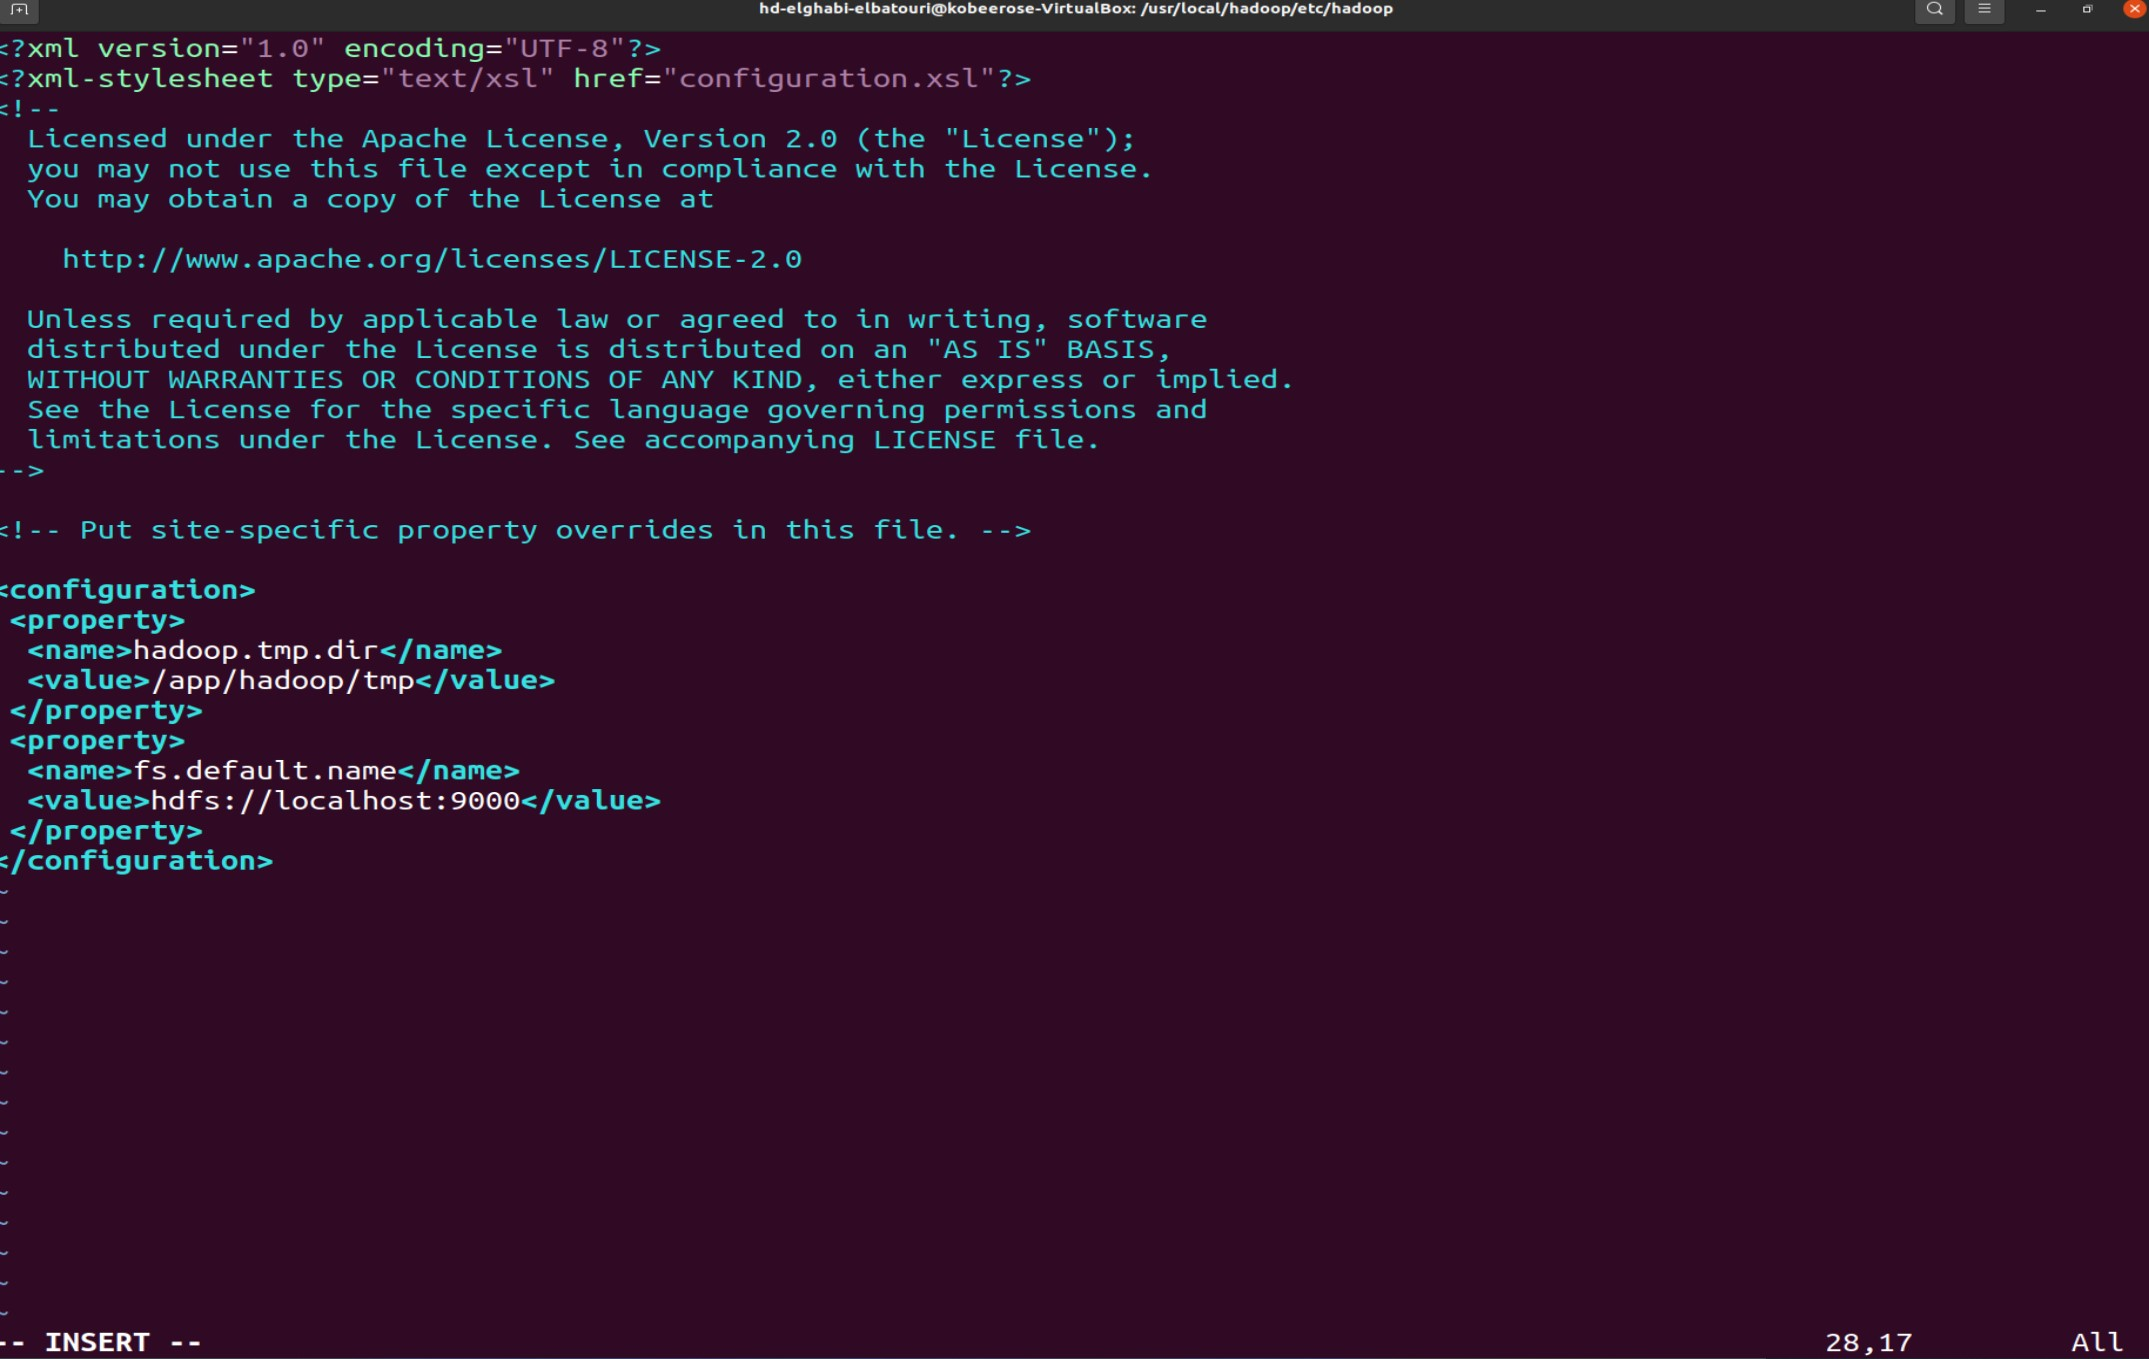
\includegraphics[width=1\linewidth]{Big_Data/Hadoop/Apache Hadoop Installation/core-site.xml config} 
\end{center} 
\caption{core-site.xml config} 
\end{figure} 
\FloatBarrier
\begin{figure}[!htb] 
\begin{center} 
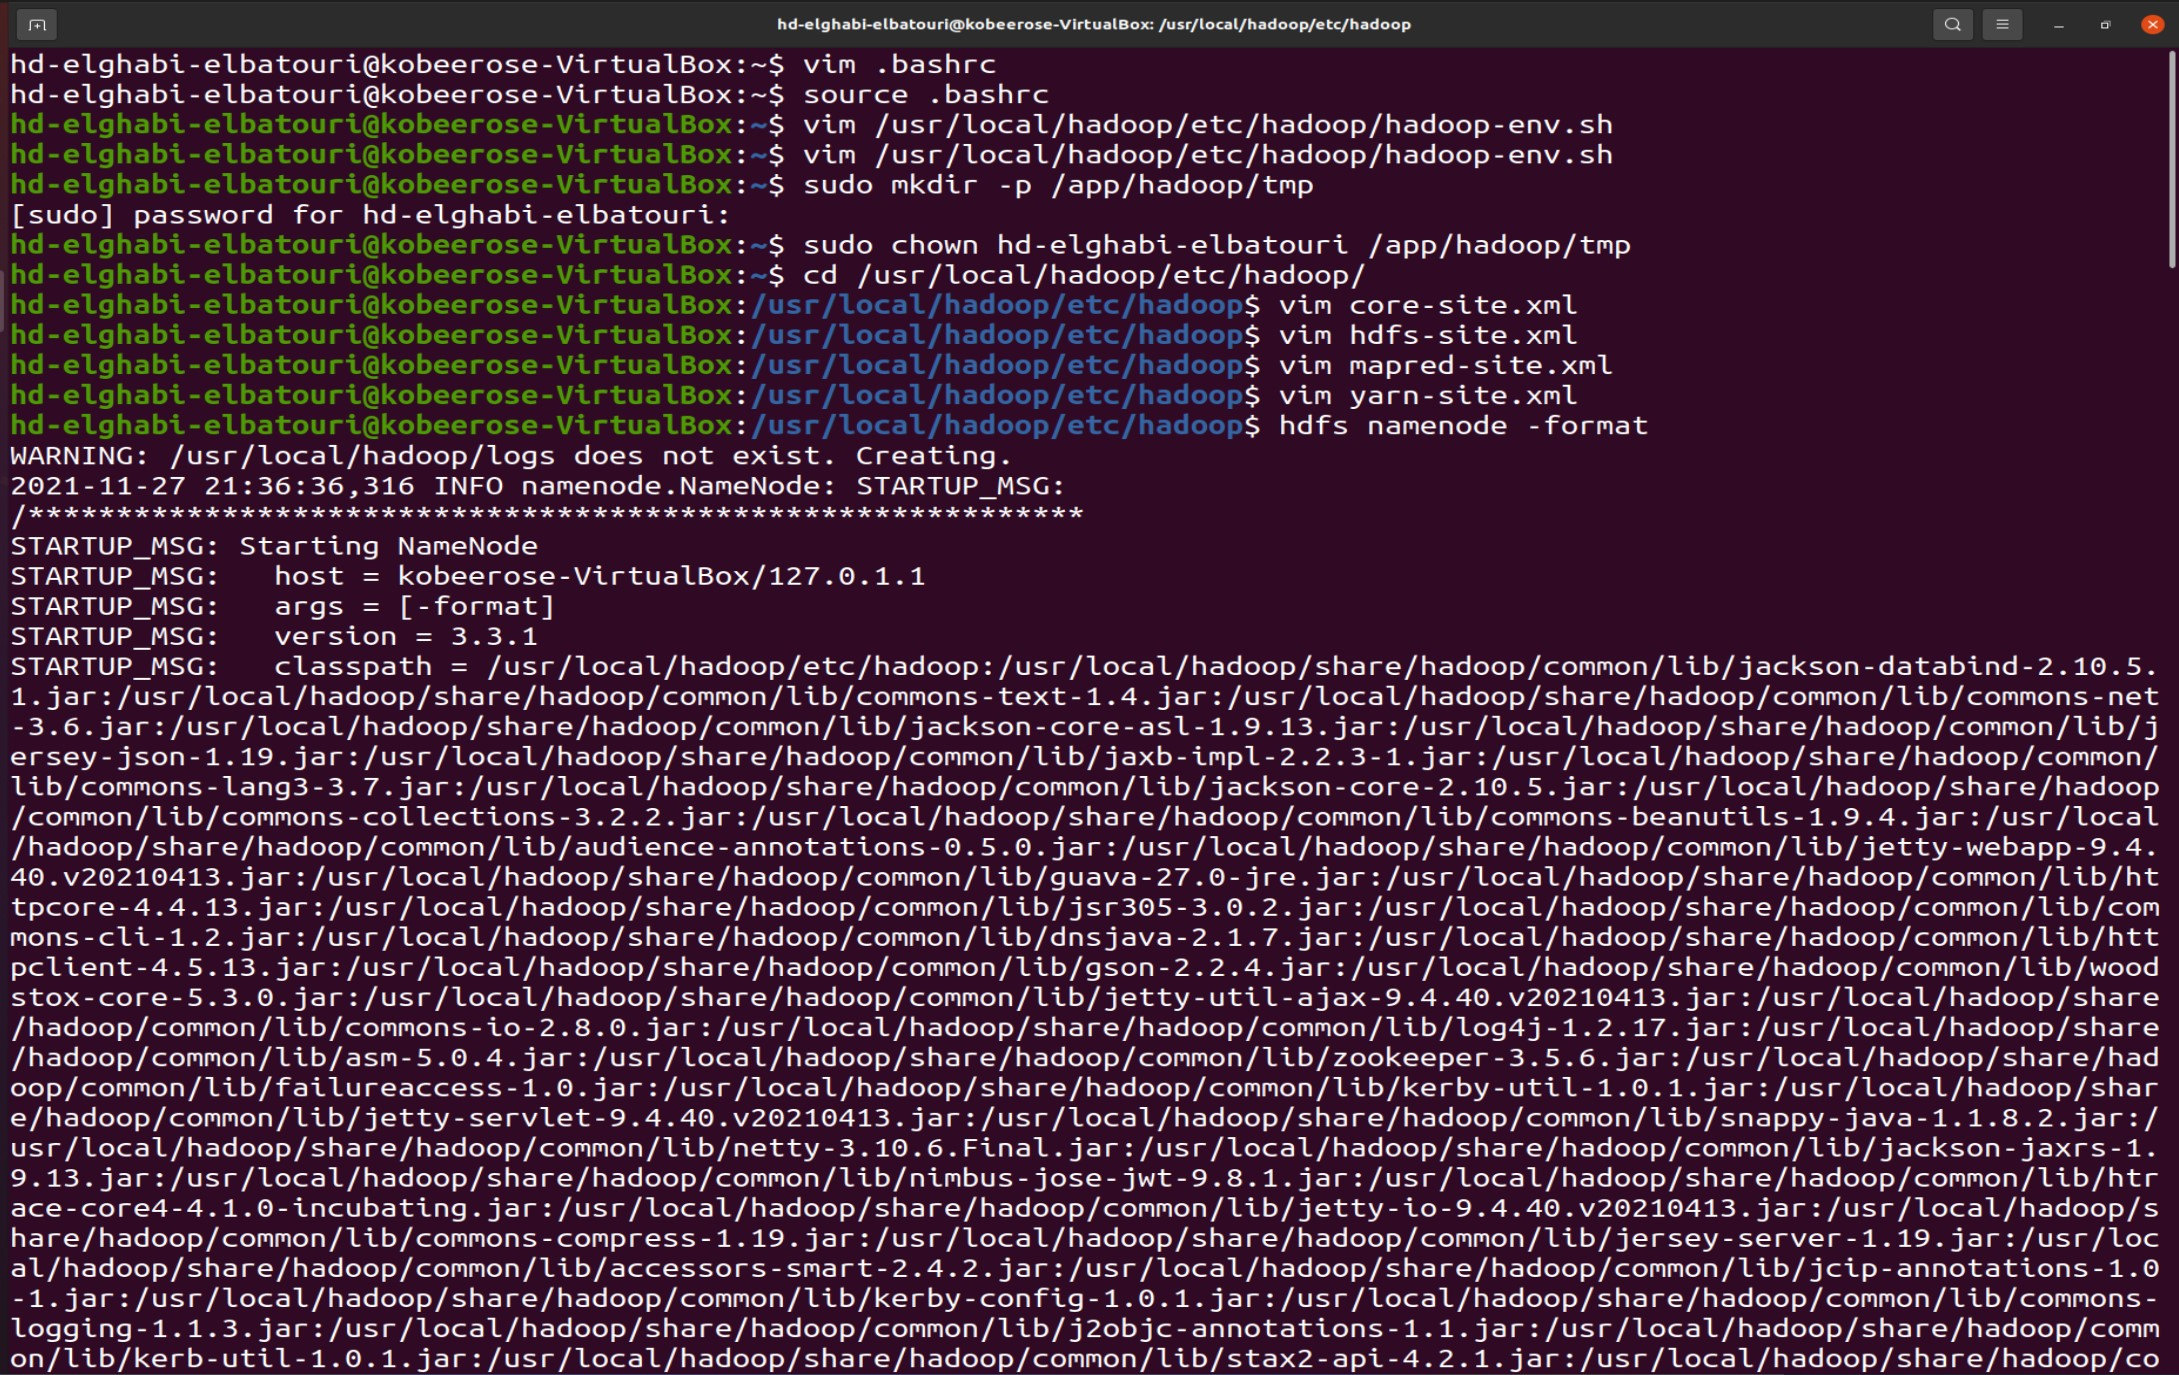
\includegraphics[width=1\linewidth]{Big_Data/Hadoop/Apache Hadoop Installation/Hadoop files configuration} 
\end{center} 
\caption{Hadoop files configuration} 
\end{figure} 
\FloatBarrier

\par Now it's time to start the newly installed single node cluster. 
\\
\begin{figure}[!htb] 
\begin{center} 
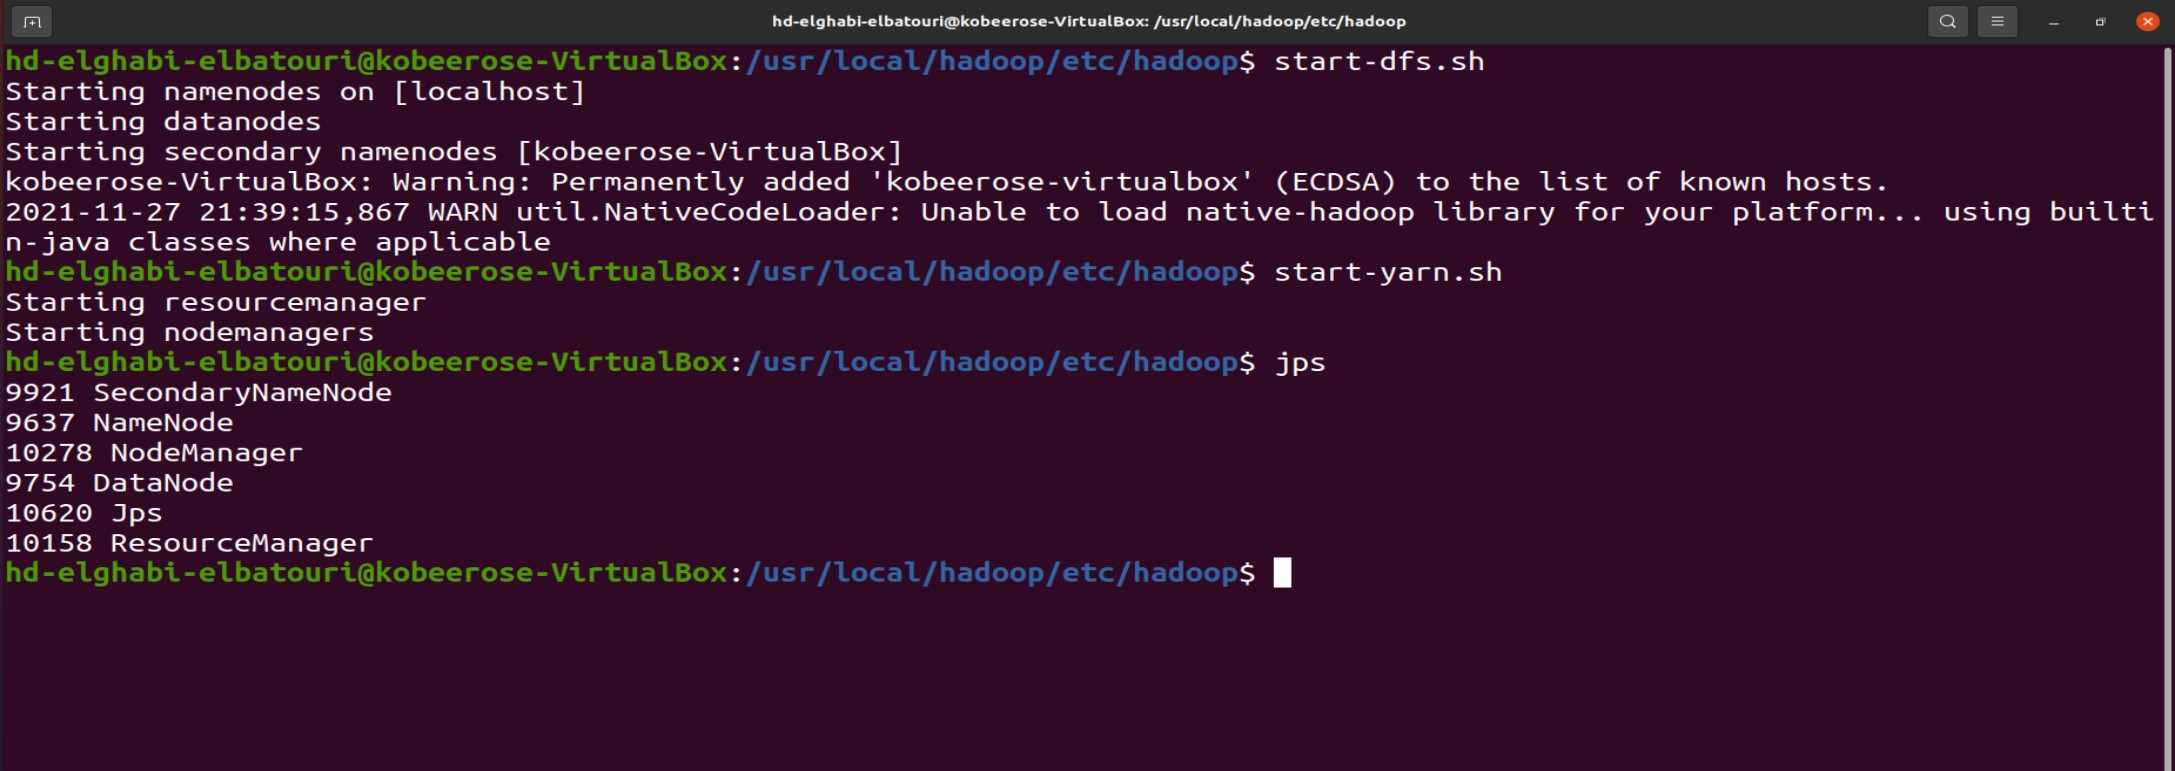
\includegraphics[width=1\linewidth]{Big_Data/Hadoop/Apache Hadoop Installation/Starting 1node Cluster} 
\end{center} 
\caption{Starting 1node Cluster} 
\end{figure} 
\FloatBarrier

\par Access Hadoop's graphical interfaces via the browser.
\\
\begin{figure}[!htb] 
\begin{center} 
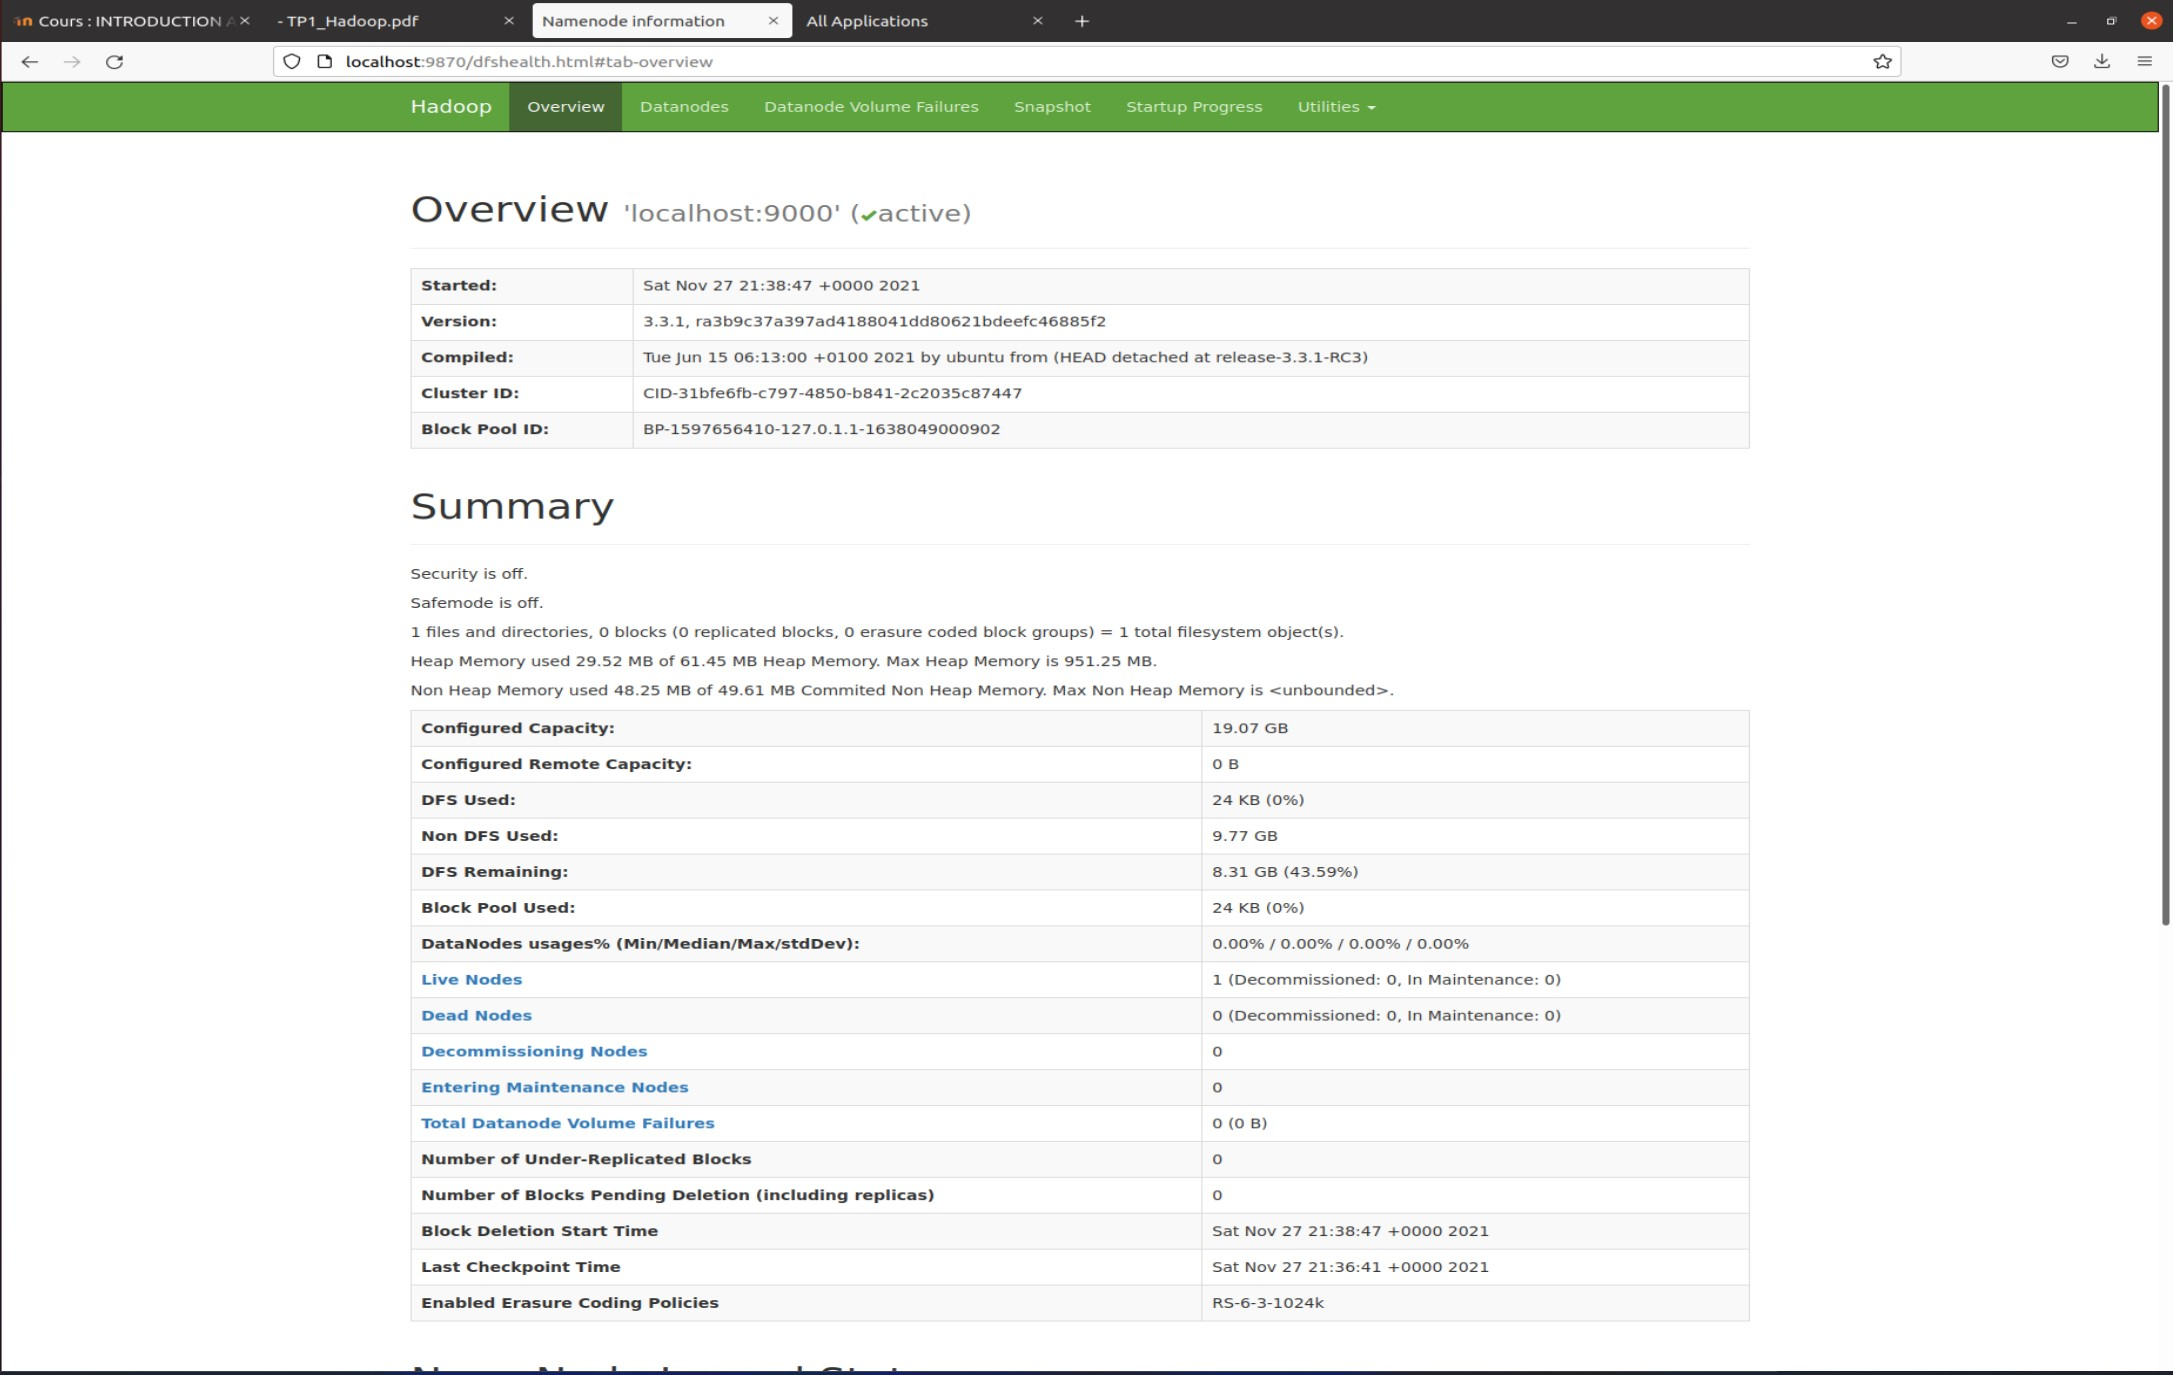
\includegraphics[width=1\linewidth]{Big_Data/Hadoop/Apache Hadoop Installation/Hadoop interface on port 9870} 
\end{center} 
\caption{Hadoop interface on port 9870} 
\end{figure} 
\FloatBarrier
\\
\begin{figure}[!htb] 
\begin{center} 
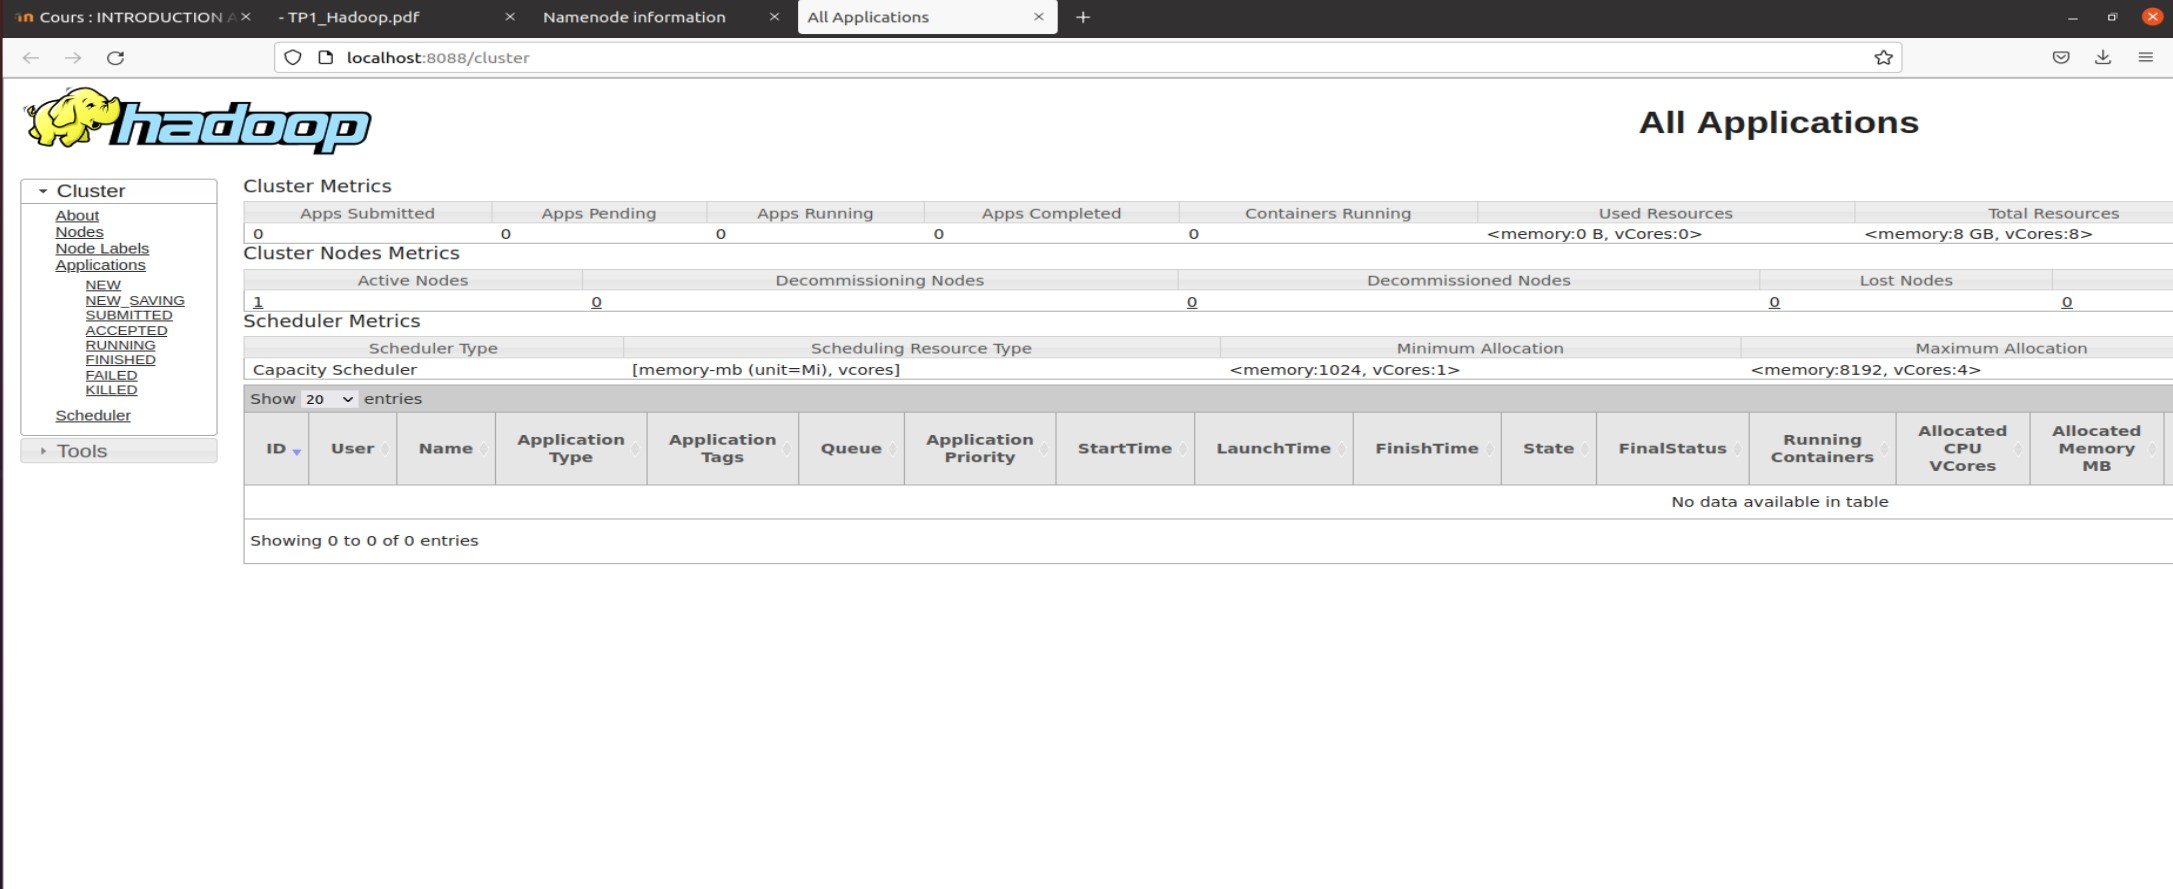
\includegraphics[width=1\linewidth]{Big_Data/Hadoop/Apache Hadoop Installation/ResourceManager Interface} 
\end{center} 
\caption{ResourceManager Interface} 
\end{figure} 
\FloatBarrier




\end{spacing}

\chapter{Pre-Requirementsuration Setup}
\par Now whit our envirement ready to use, we will be installing Openstack Victoria that will help us to build our private cloud, RabbitMQ as message streaming, broker and messaging queue implementation that Openstack services will use in order to communicate since we are in the context of a distributed system. And finally Memcached to ensure that our system will have a caching protocol that fit our distributed system; caching is used to keep important and most demanded information fast to access an store it in memory rather than the hard-drive.
\begin{spacing}{1.2}
%note en bas de page
\section{Openstack Victoria}

\par The installation of centos-release-openstack-victoria, rabbitmq-server and memcached is done via dnf. A
After installation is complete, an update of the CentOS System is required. 
\\
\begin{figure}[!htb] 
\begin{center} 
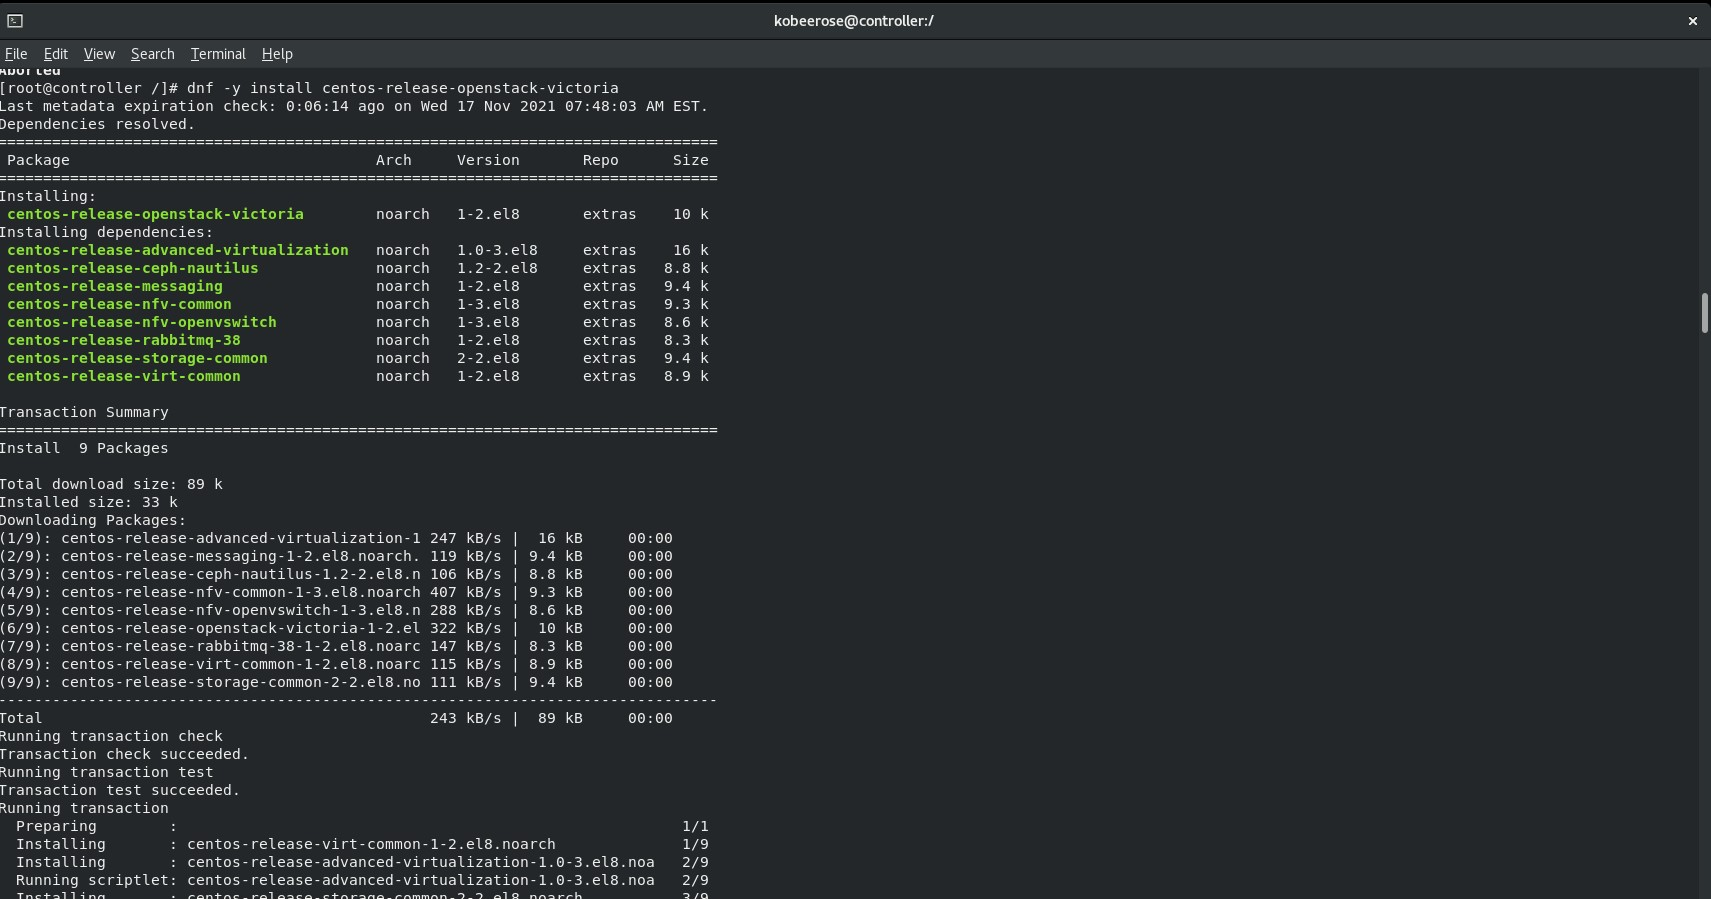
\includegraphics[width=1\linewidth]{Cloud/Pre-Requirements/Installing openstack-victoria} 
\end{center} 
\caption{Installing openstack-victoria} 
\end{figure}  \FloatBarrier
\\
\\
\begin{figure}[!htb] 
\begin{center} 
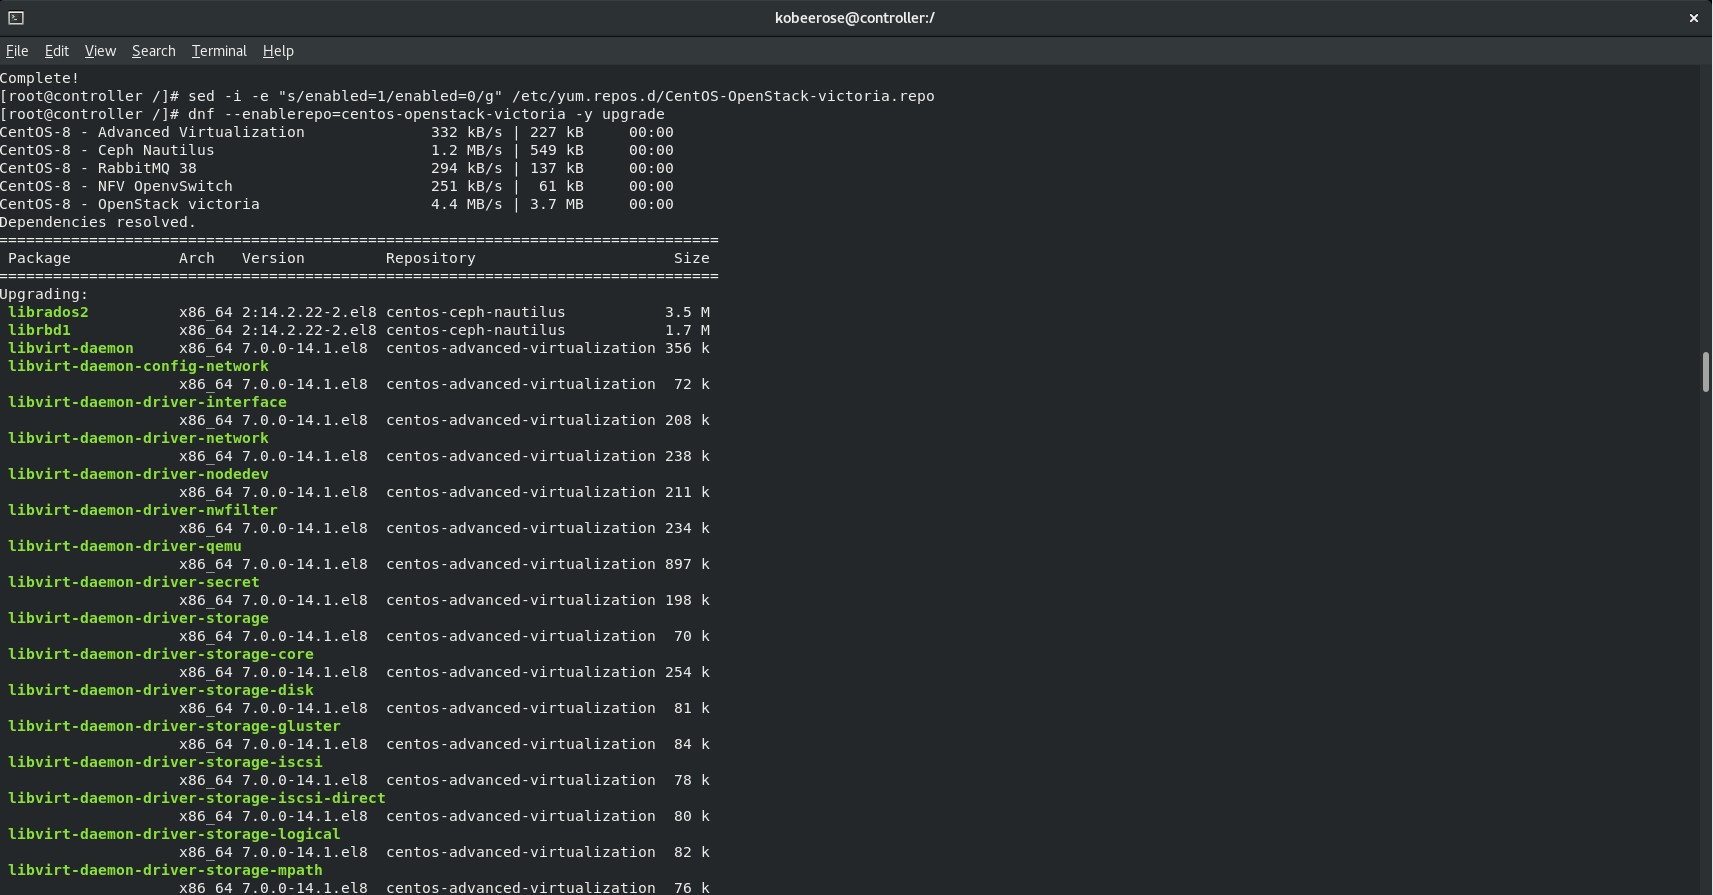
\includegraphics[width=1\linewidth]{Cloud/Pre-Requirements/Add Openstack Repo _ Upgrade CentOS System} 
\end{center} 
\caption{Add Openstack Repo _ Upgrade CentOS System} 
\end{figure}  \FloatBarrier
\\

\section{Installation of RabbitMQ, Memcached.}

\par First of all we need to install RabbitMQ server
\\
\begin{figure}[!htb] 
\begin{center} 
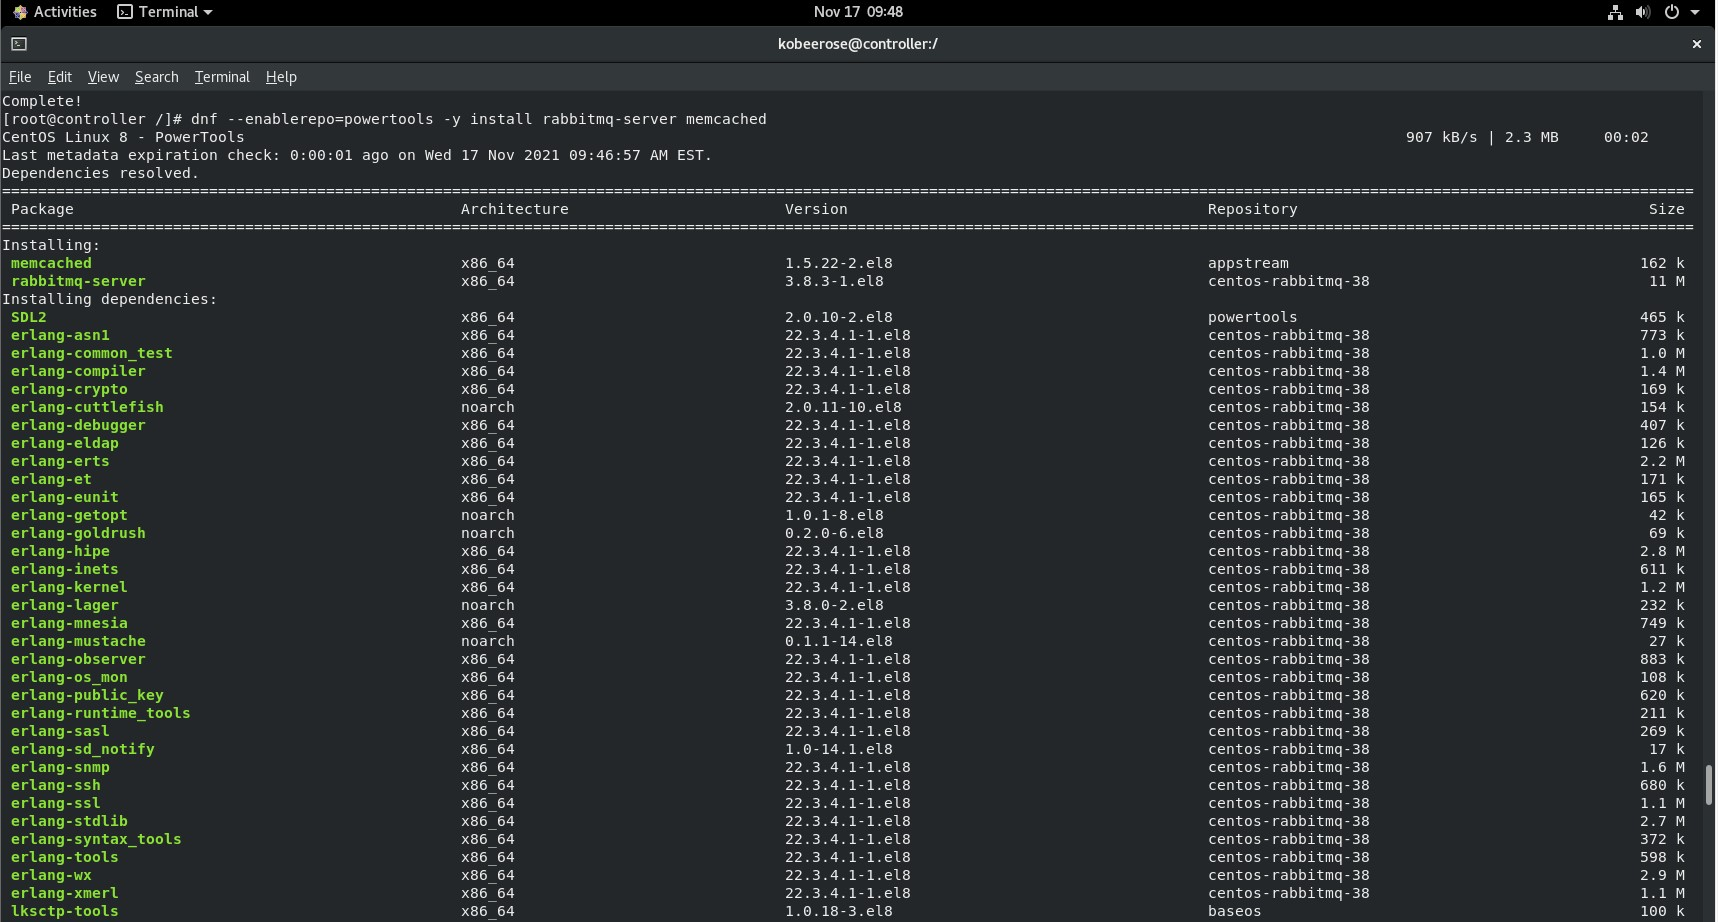
\includegraphics[width=1\linewidth]{Cloud/Pre-Requirements/Installing rabbitmq-server} 
\end{center} 
\caption{Installing rabbitmq-server} 
\end{figure}  \FloatBarrier
\\
\par We are going to change in the file /etc/my.cnf.d/mariadb-server.cnf the default value 151
which is not sufficient in the Openstack environment. And to consider the modifications, we
let's restart and enable mariadb rabbitmq-server and memcached. 
\\
\begin{figure}[!htb] 
\begin{center} 
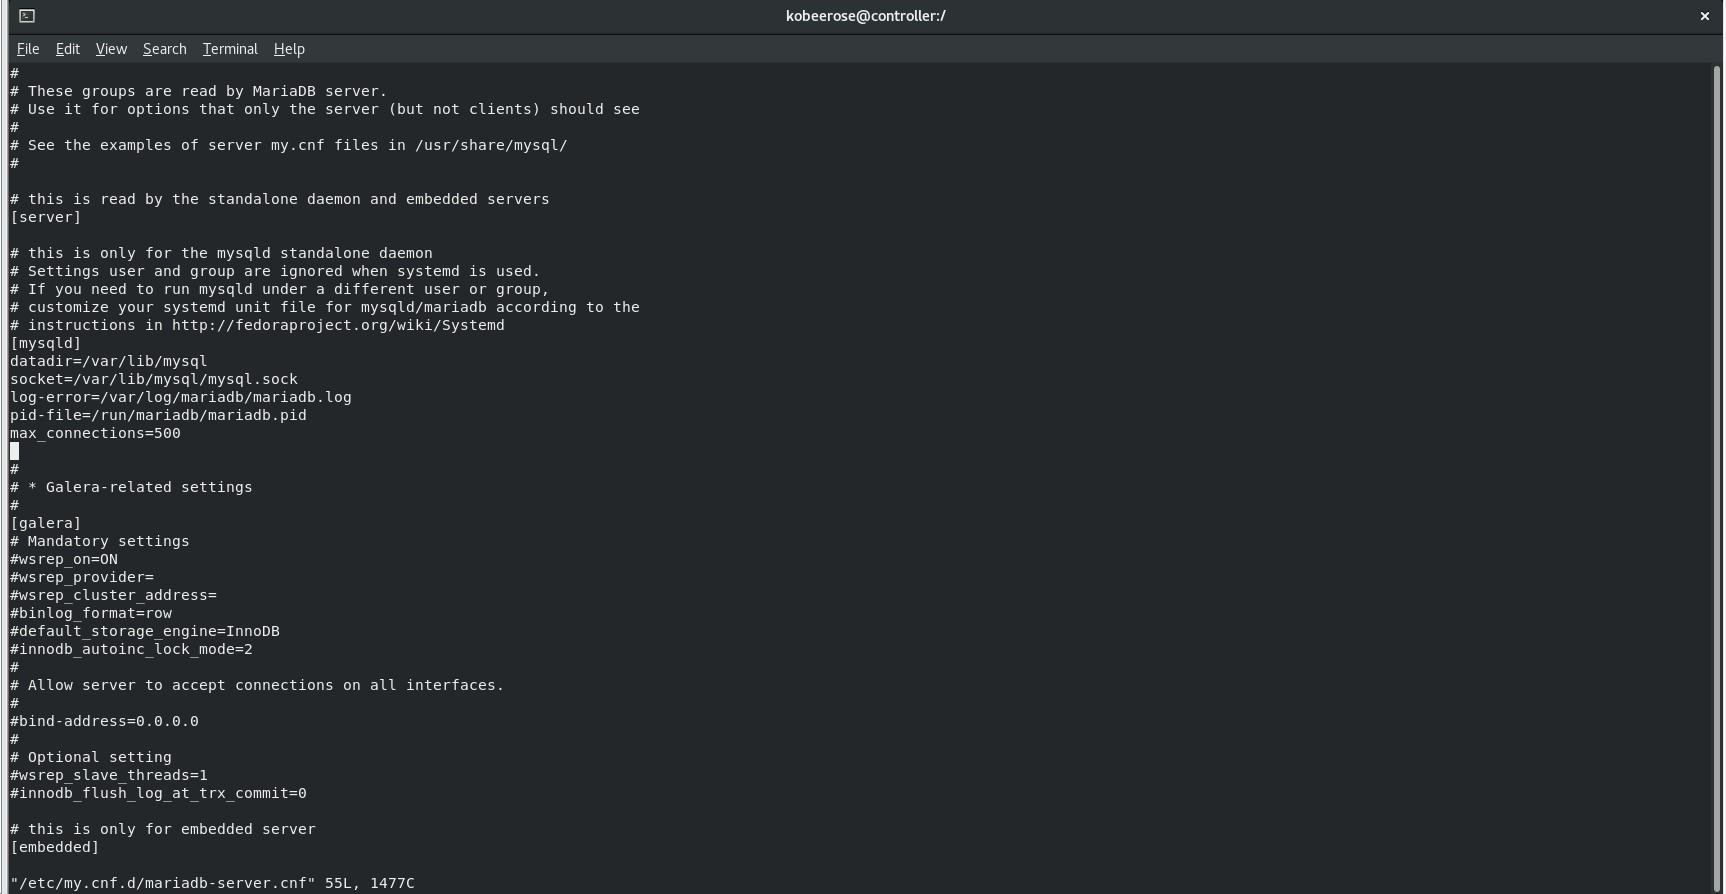
\includegraphics[width=1\linewidth]{Cloud/Pre-Requirements/changing max_connections} 
\end{center} 
\caption{changing max connections} 
\end{figure}  \FloatBarrier
\\
\par now we persue with configuring the memcached file in order to listen to all
\\
\begin{figure}[!htb] 
\begin{center} 
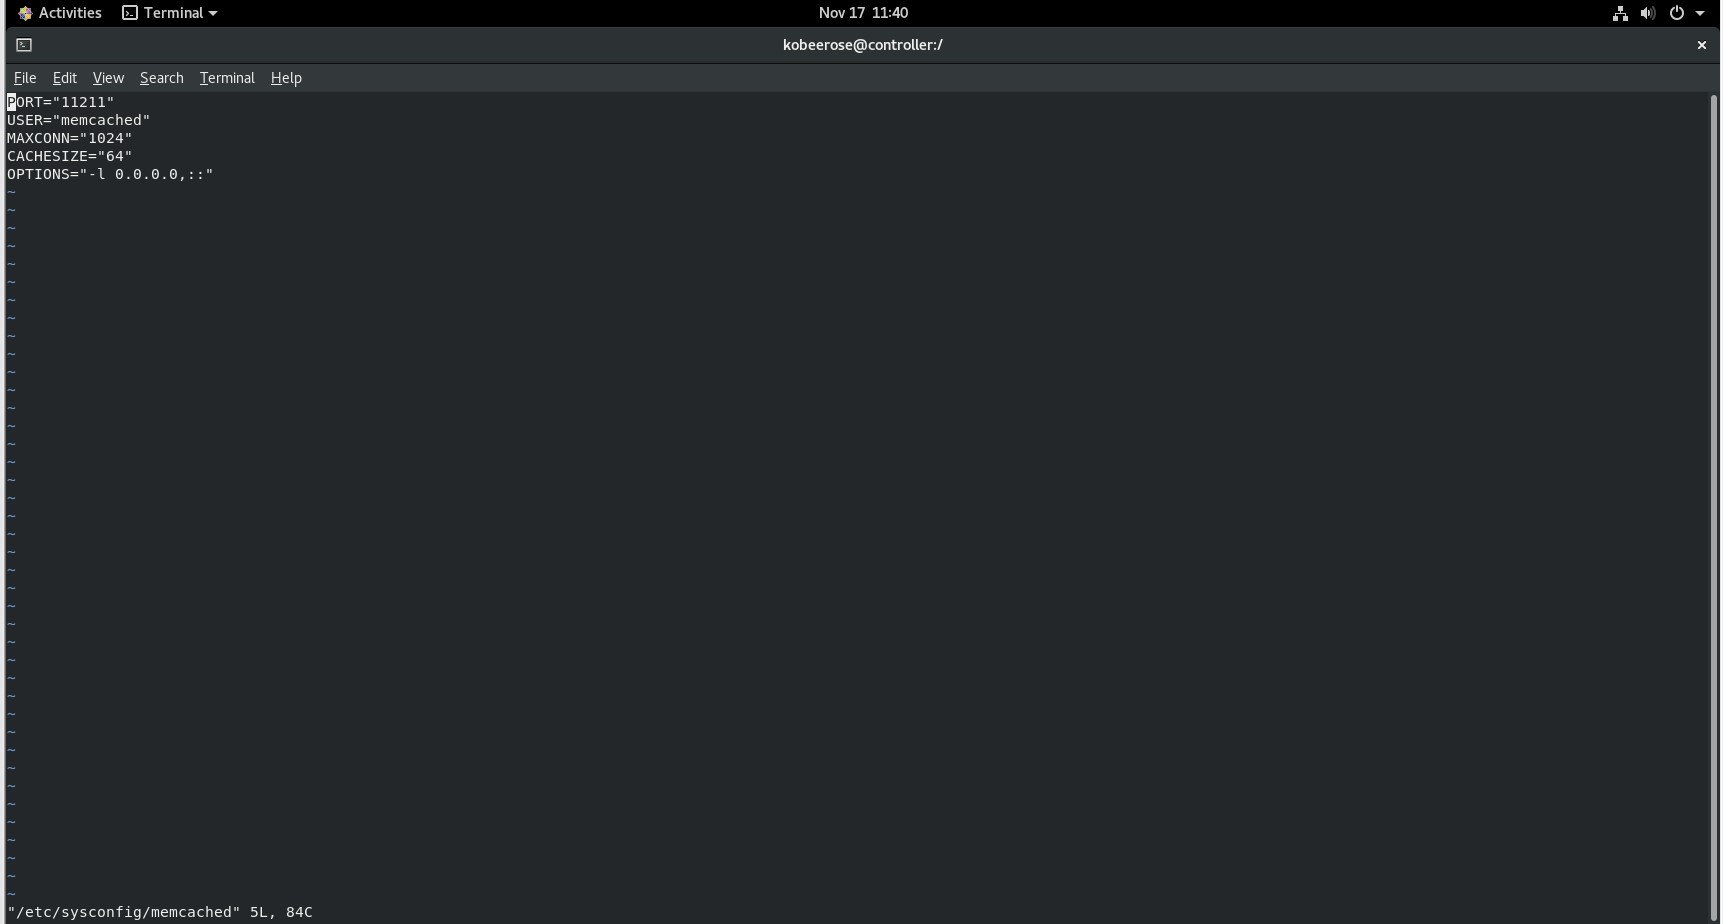
\includegraphics[width=1\linewidth]{Cloud/Pre-Requirements/memcached config} 
\end{center} 
\caption{memcached config} 
\end{figure}  \FloatBarrier
\\
\section{rabbitmqctl config }
\\
\par After that, we will add a new openstack user, define a password for him.
, also give it all the permissions and if SELinux is enabled, we have to change the policy
via a rabbitmqctl.te file and We will use the checkmodule and semodule commands to verify and compile this module.
of SELinux security policy in a binary representation8 
\\
\begin{figure}[!htb] 
\begin{center} 
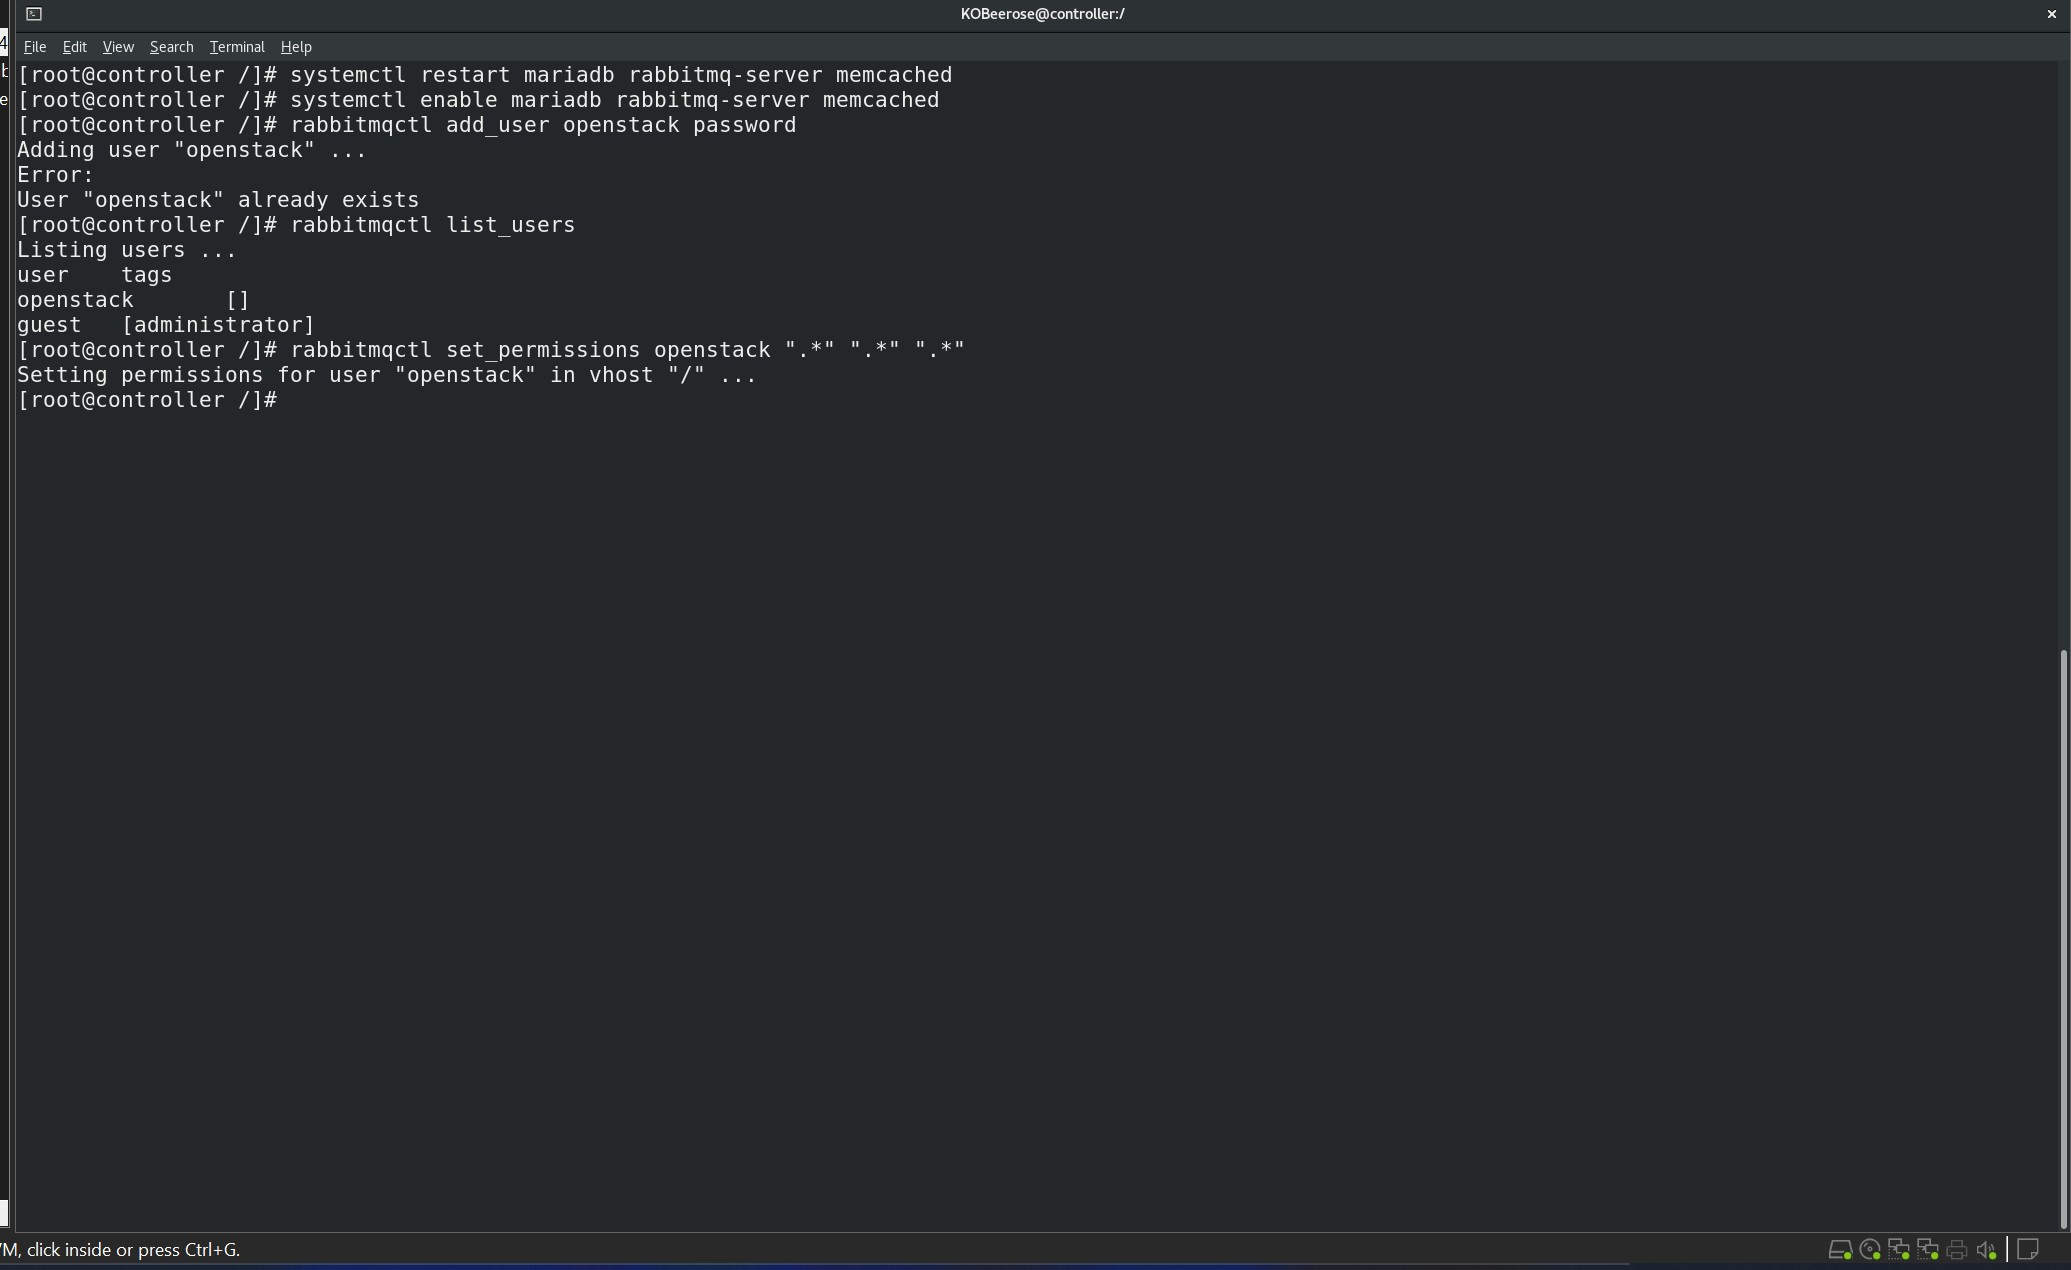
\includegraphics[width=1\linewidth]{Cloud/Pre-Requirements/Creating a new openstack user} 
\end{center} 
\caption{Creating a new openstack user} 
\end{figure}  \FloatBarrier
\\


\par Allowing mysql service, the port 5672 service and reloading the firewall.\\
\\
\begin{figure}[!htb] 
\begin{center} 
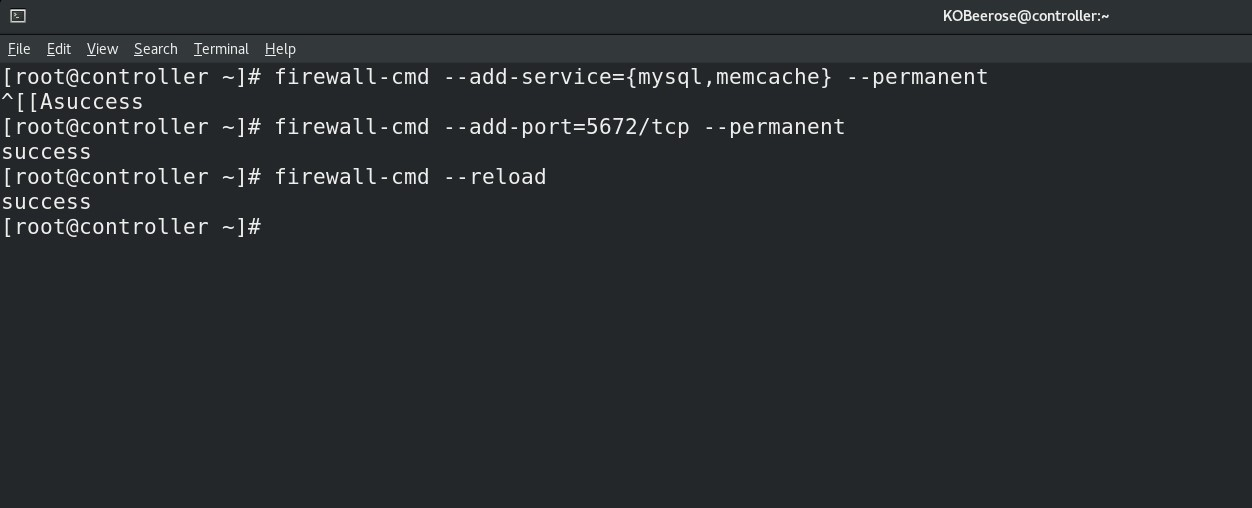
\includegraphics[width=.8\linewidth]{Cloud/Pre-Requirements/Allowing ports for services.} 
\end{center} 
\caption{Allowing ports for services.} 
\end{figure}  \FloatBarrier
\\


\end{spacing}
 
\chapter{Keystone Configuration}
\par based on the documentation, Keystone is an OpenStack service that provides API client authentication, service discovery, and distributed multi-tenant authorization by implementing OpenStack’s Identity API; which mean that keystone is the service that will be used as the authentication service and also will provide each user the services that he can use. And this section is dedicated to Keystone installation and configuration.
\begin{spacing}{1.2}
%note en bas de page
\section{Add a User and Database on MariaDB for Keystone}

\par In this section, we will install and configure OpenStack Identity Service (Keystone). We
are going to connect to MariaDb so that we can add a user and a database
for Keystone. 
\\
\begin{figure}[!htb] 
\begin{center} 
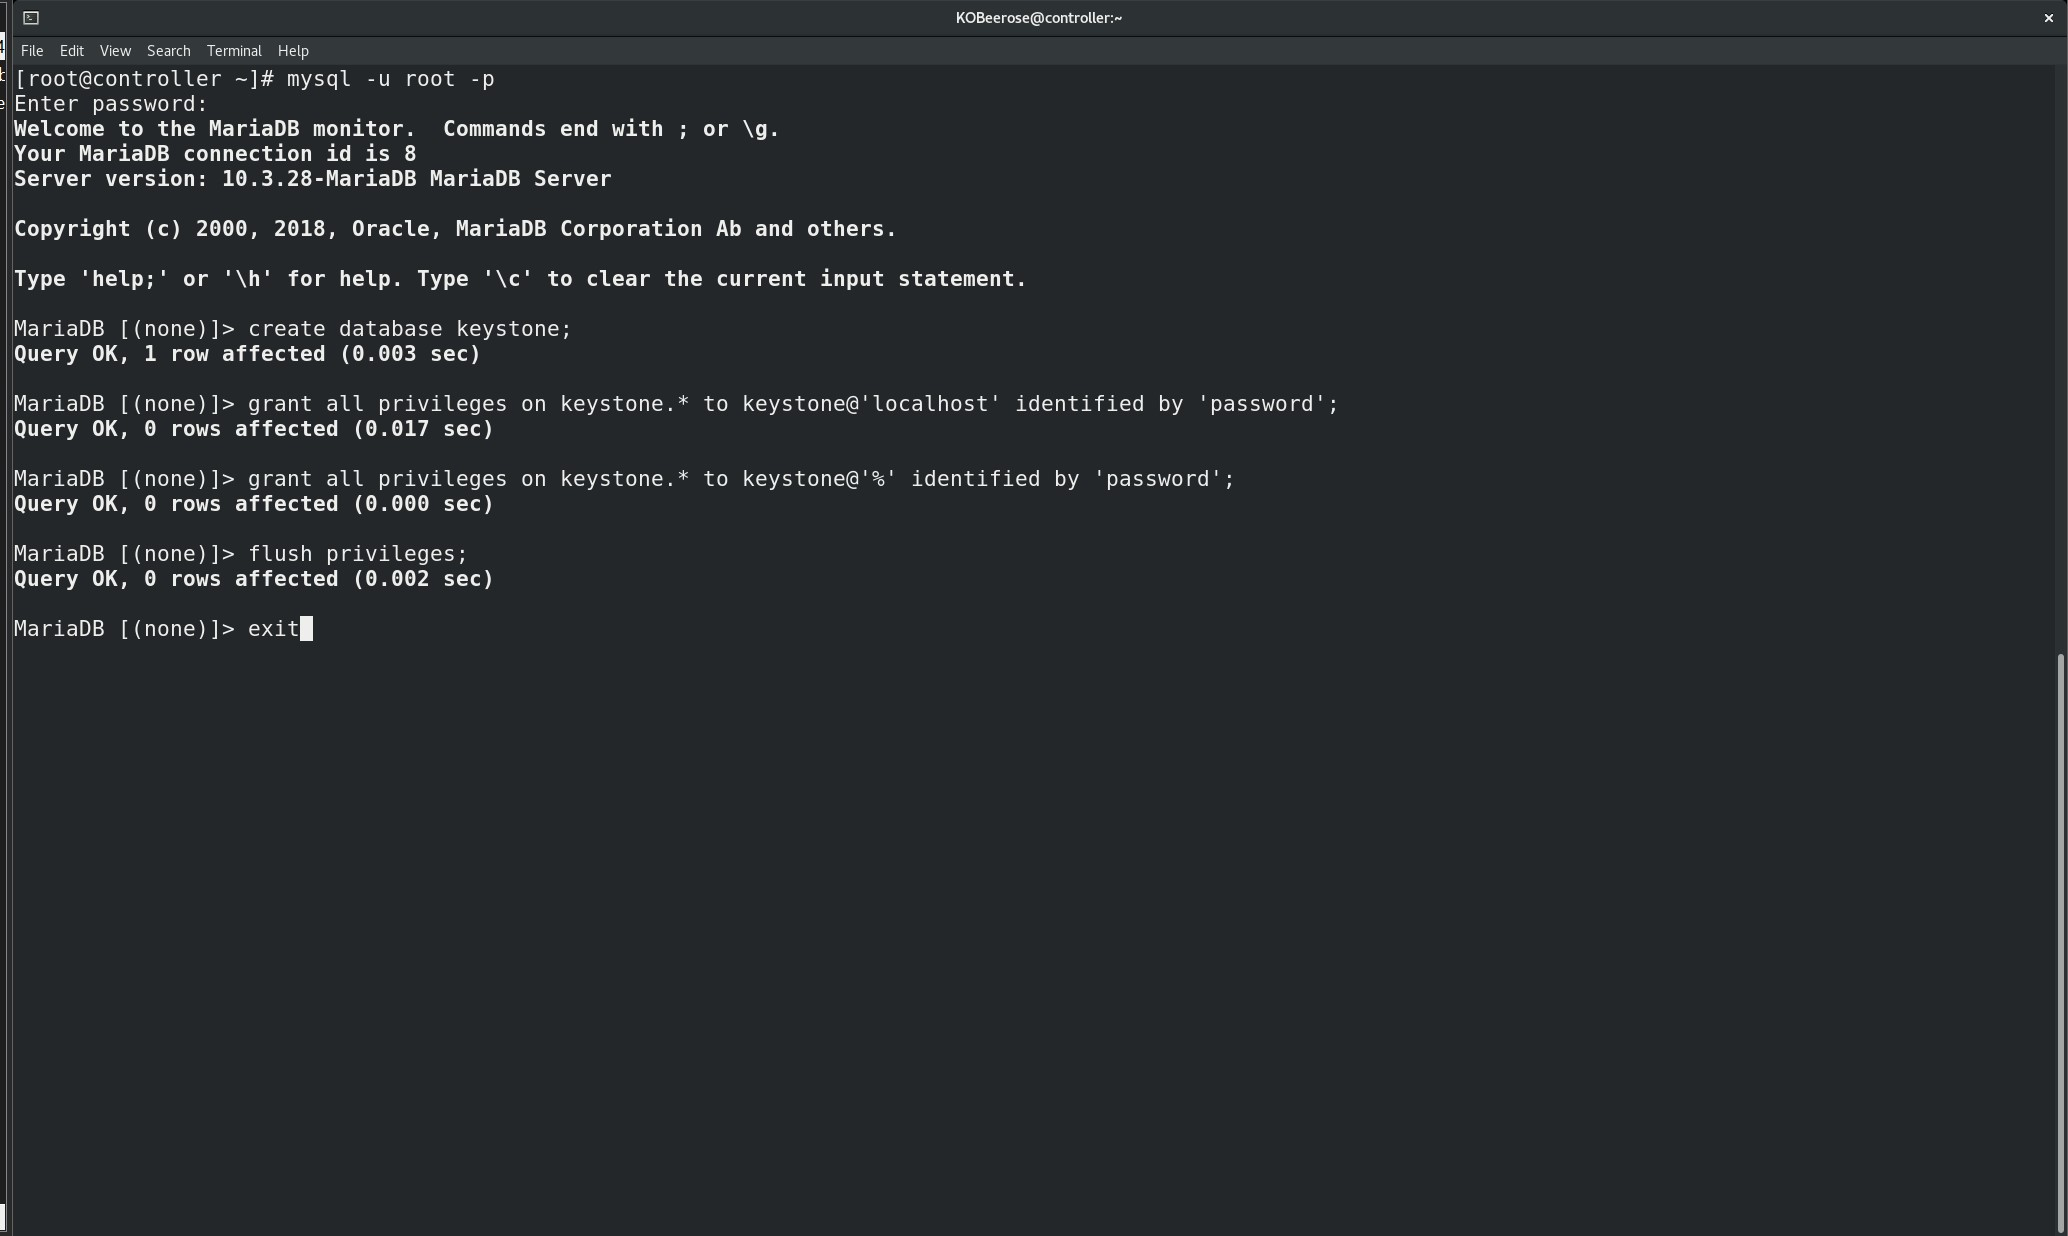
\includegraphics[width=1\linewidth]{Cloud/Configure Keystone #1/Add a user and DB for Keystone} 
\end{center} 
\caption{Add a user and DB for Keystone} 
\end{figure}  \FloatBarrier
\\


\section{Installing Keystone}

\par To install Keystone, we need to install many packages as shown in the
figure below: 
\\
\begin{figure}[!htb] 
\begin{center} 
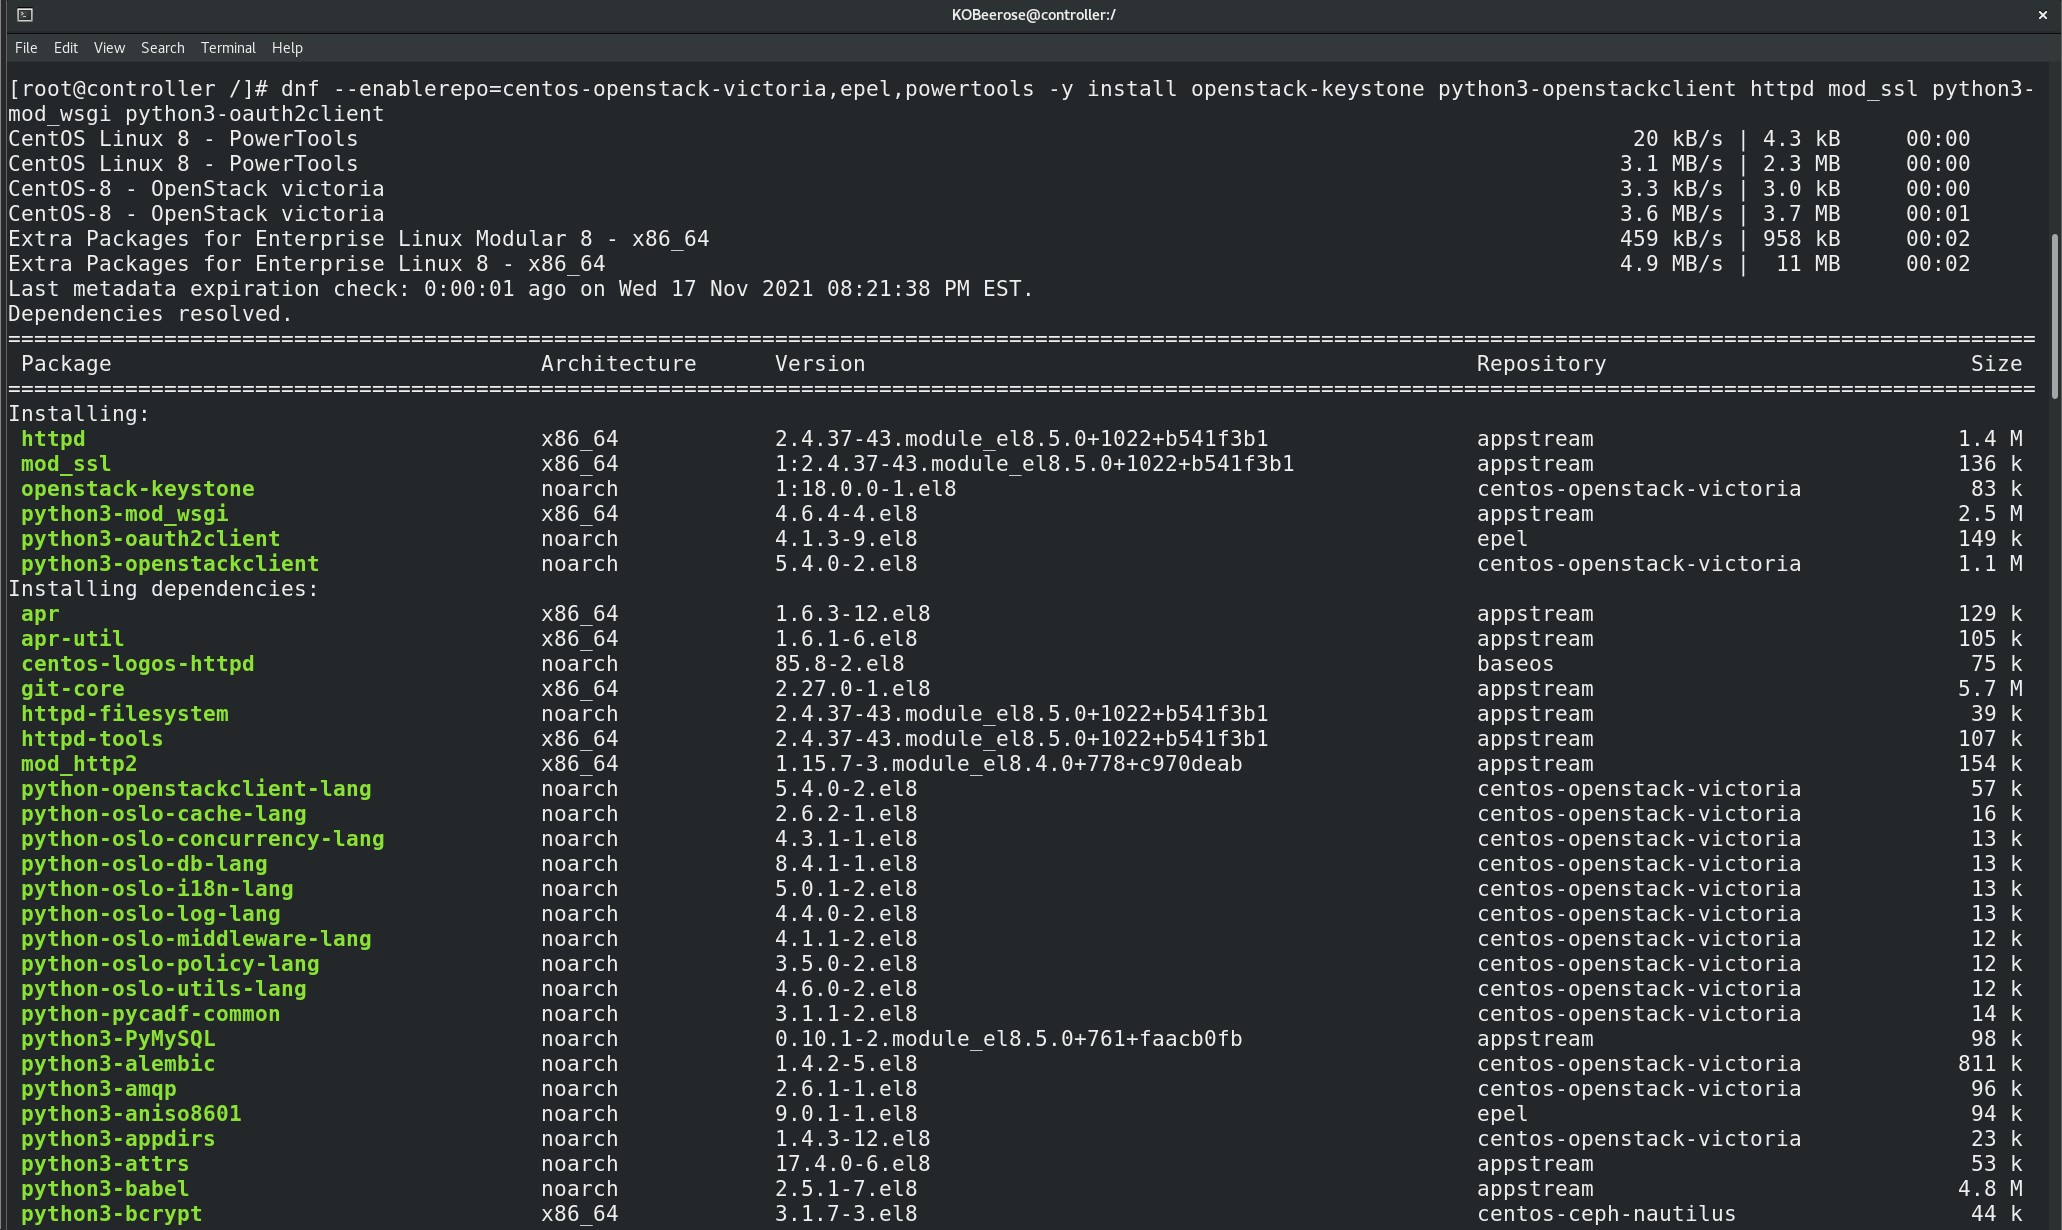
\includegraphics[width=1\linewidth]{Cloud/Configure Keystone #1/Installing EPEL, powertools} 
\end{center} 
\caption{Installing EPEL, powertools} 
\end{figure}  \FloatBarrier
\\


\section{Configure Keystone.}

\par To configure Keystone, we will specify the Memcache server, specify the information
MariaDB connection and comment on the Provider Fernet .\\

\\
\begin{figure}[!htb] 
\begin{center} 
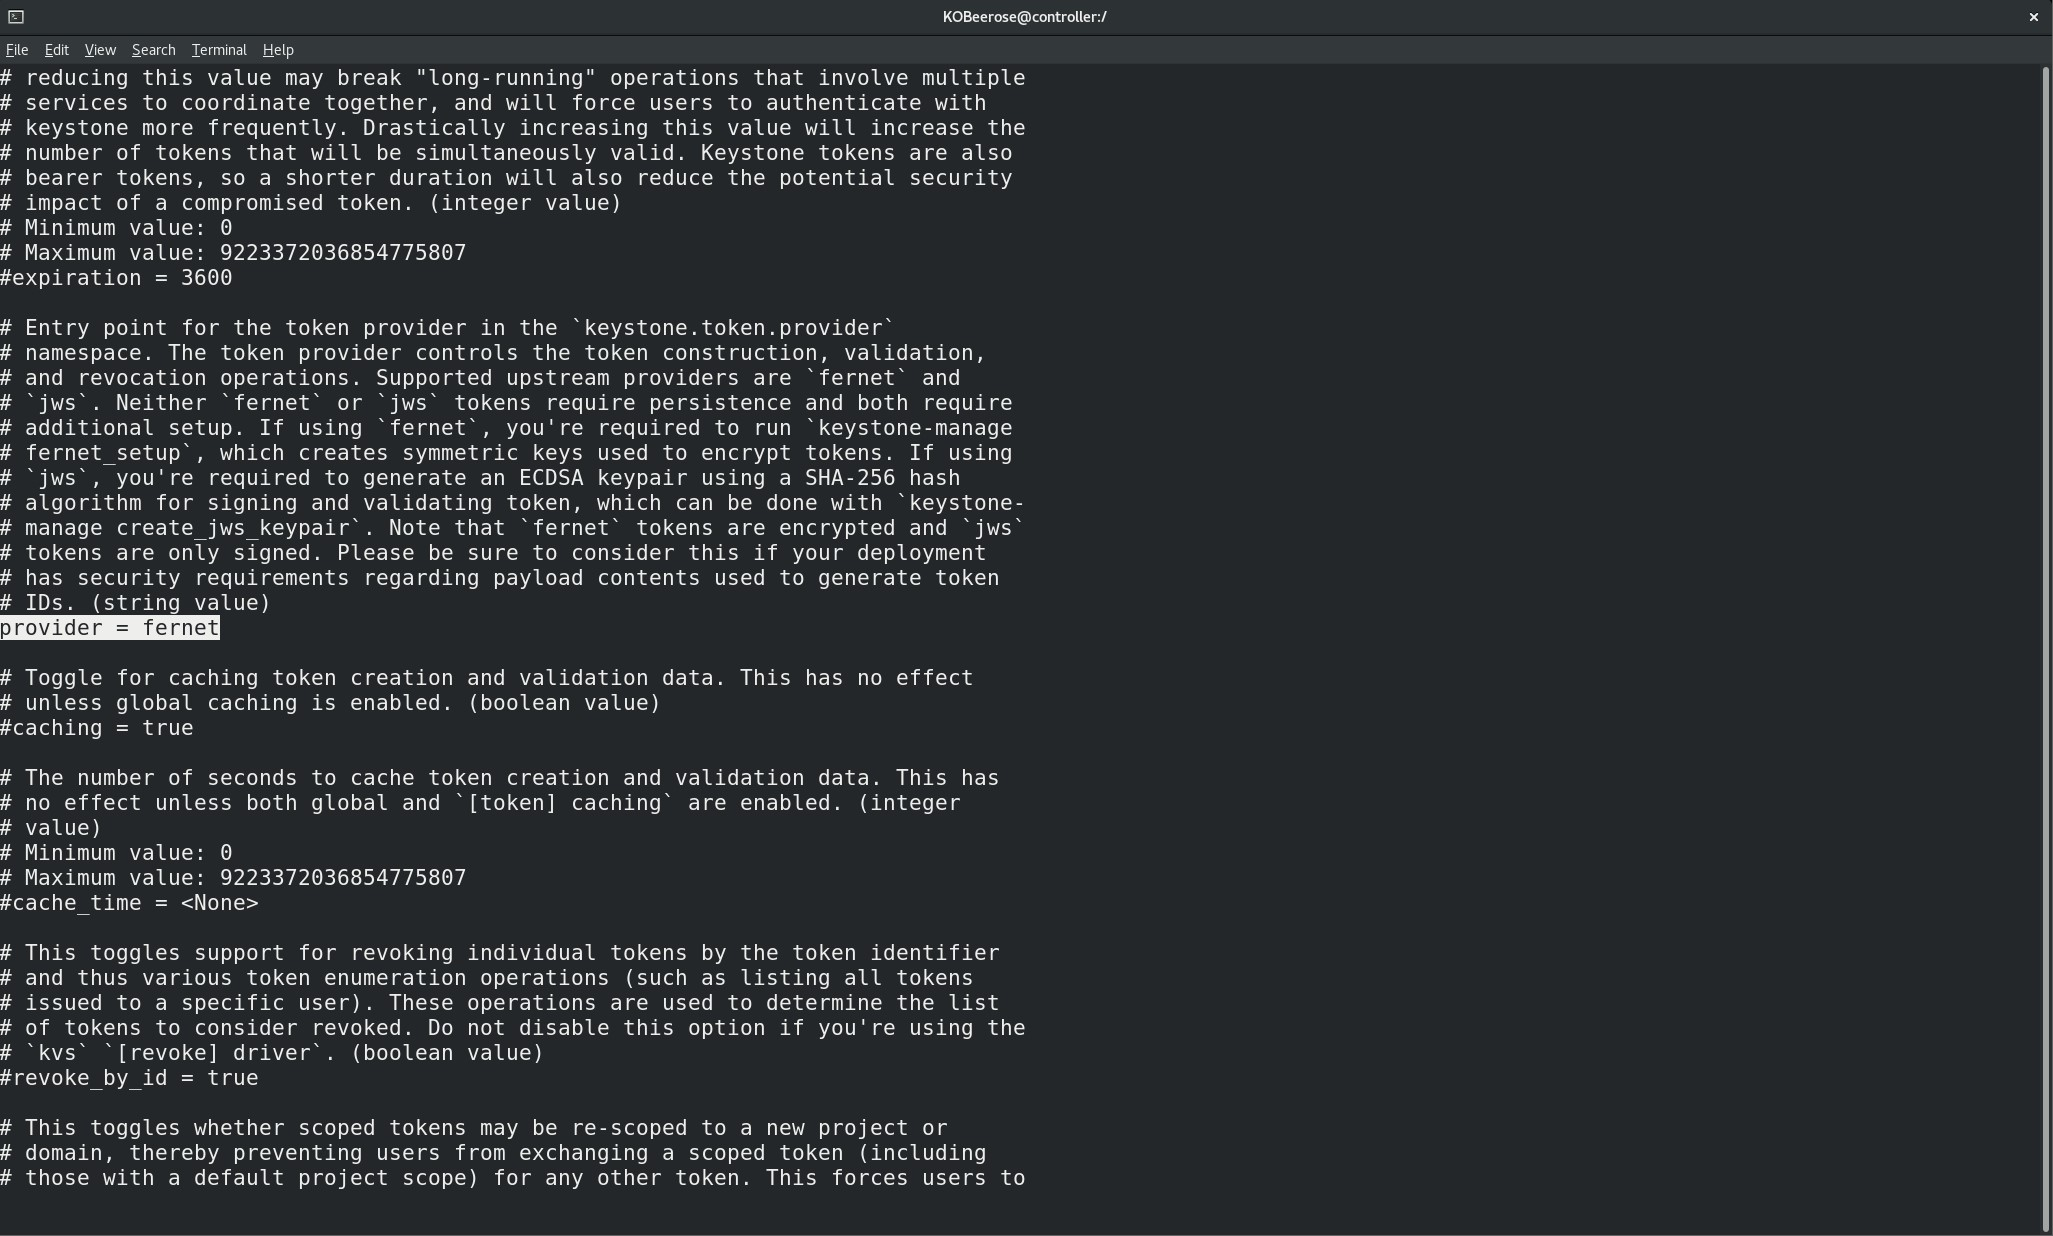
\includegraphics[width=1\linewidth]{Cloud/Configure Keystone #1/keystone.conf file} 
\end{center} 
\caption{keystone.conf file} 
\end{figure}  \FloatBarrier
\\
\par After having synchronized Keystone, we will initialize the keys, define Keystone Host and
run the keystone-manage bootstrap command to create a user, project, and role, and
assign roles. By default, the names of these new resources will be called admin. 
\\
\begin{figure}[!htb] 
\begin{center} 
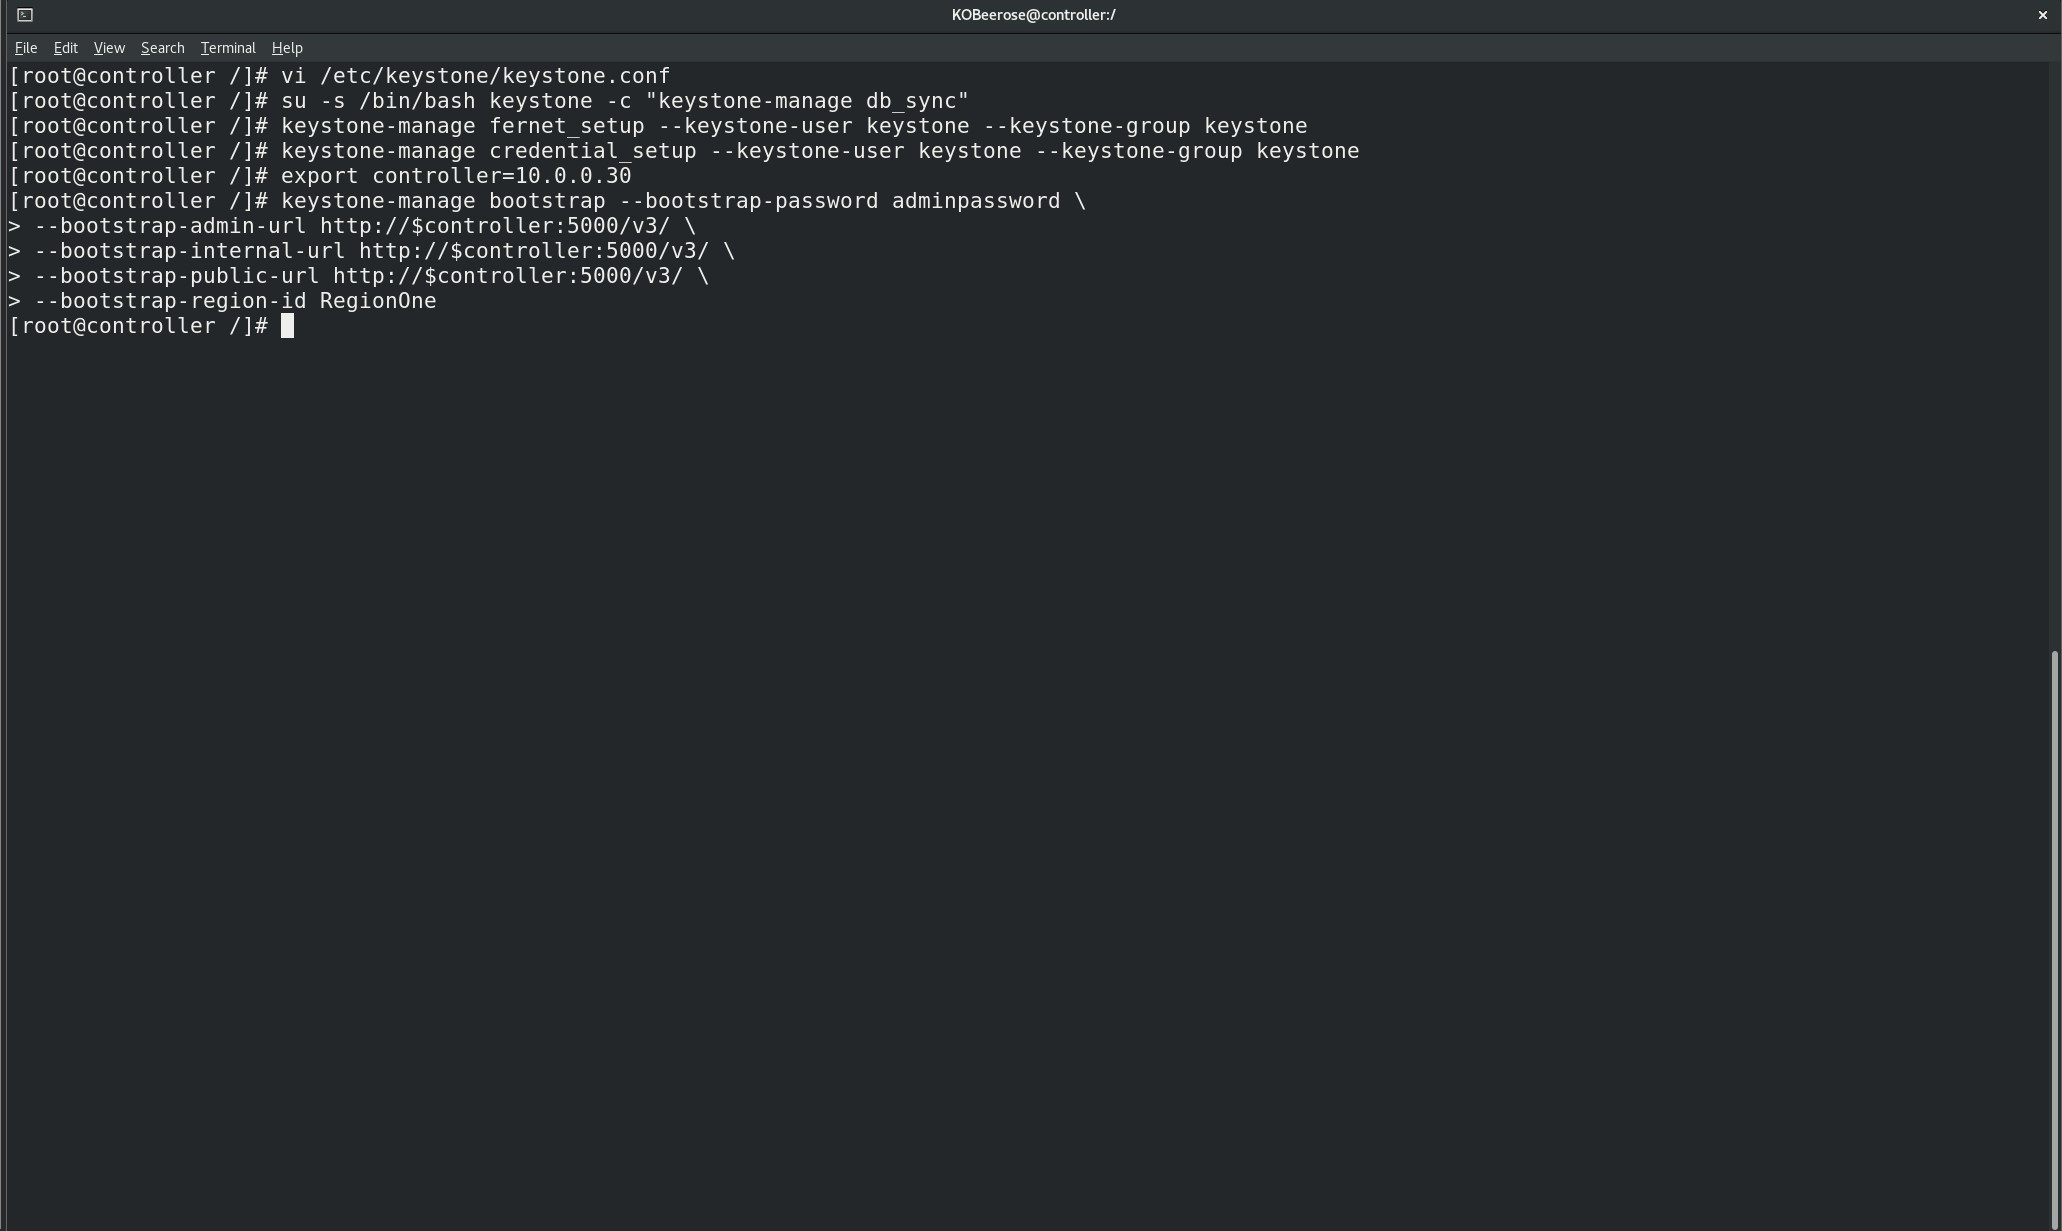
\includegraphics[width=1\linewidth]{Cloud/Configure Keystone #1/Configure Keystone} 
\end{center} 
\caption{Configure Keystone} 
\end{figure}  \FloatBarrier
\\
\section{keystone-httpd config}
\par 
As always, we need to change the boolean parameters of selinux and change the policy by creating a new module keystone-httpd.te to compile as shown below
\\
\begin{figure}[!htb] 
\begin{center} 
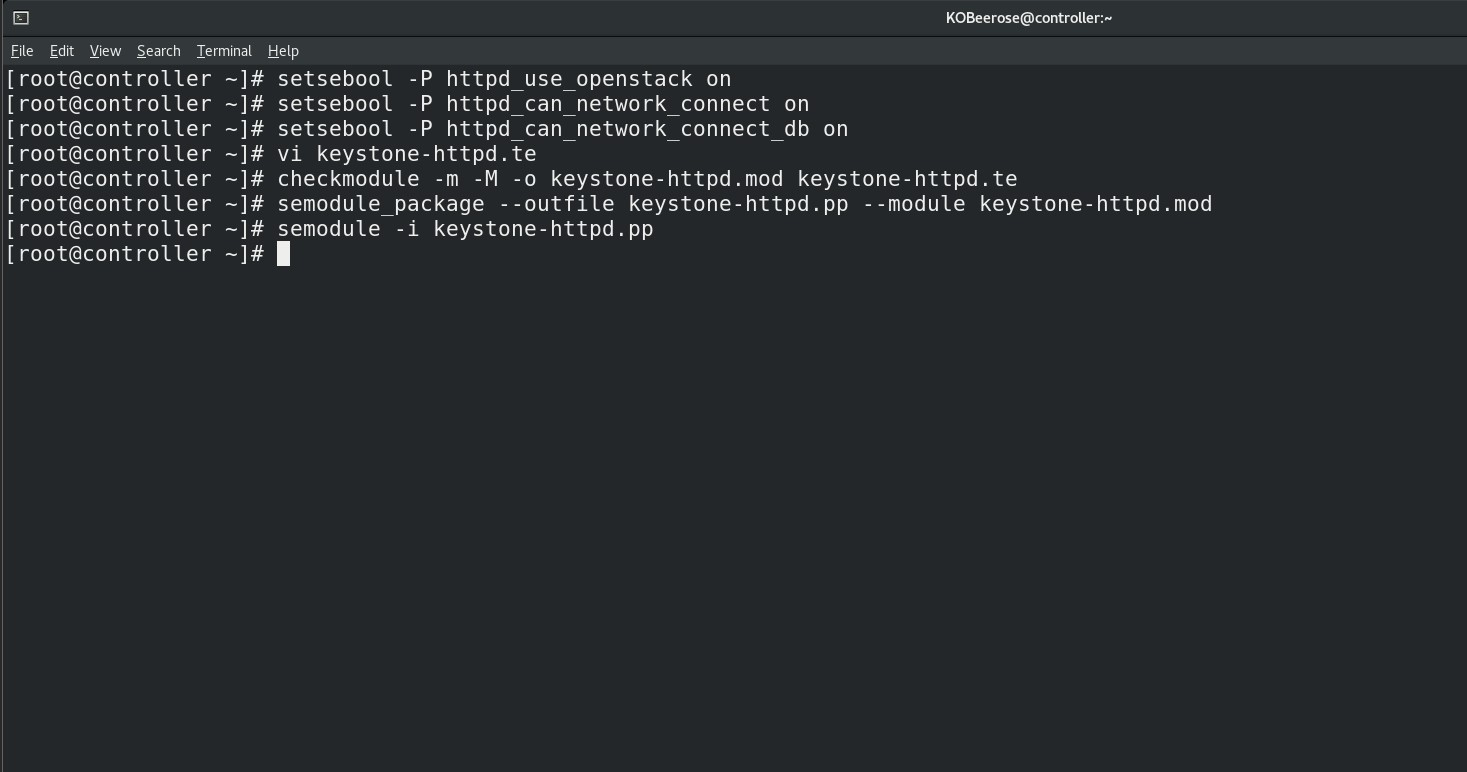
\includegraphics[width=1\linewidth]{Cloud/Configure Keystone #1/keystone-httpd config} 
\end{center} 
\caption{keystone-httpd config} 
\end{figure}  \FloatBarrier
\\
\section{Starting Apache httpd}
\par 
First step is allowing the port 5000 service and reloading the firewall.
\\
\begin{figure}[!htb] 
\begin{center} 
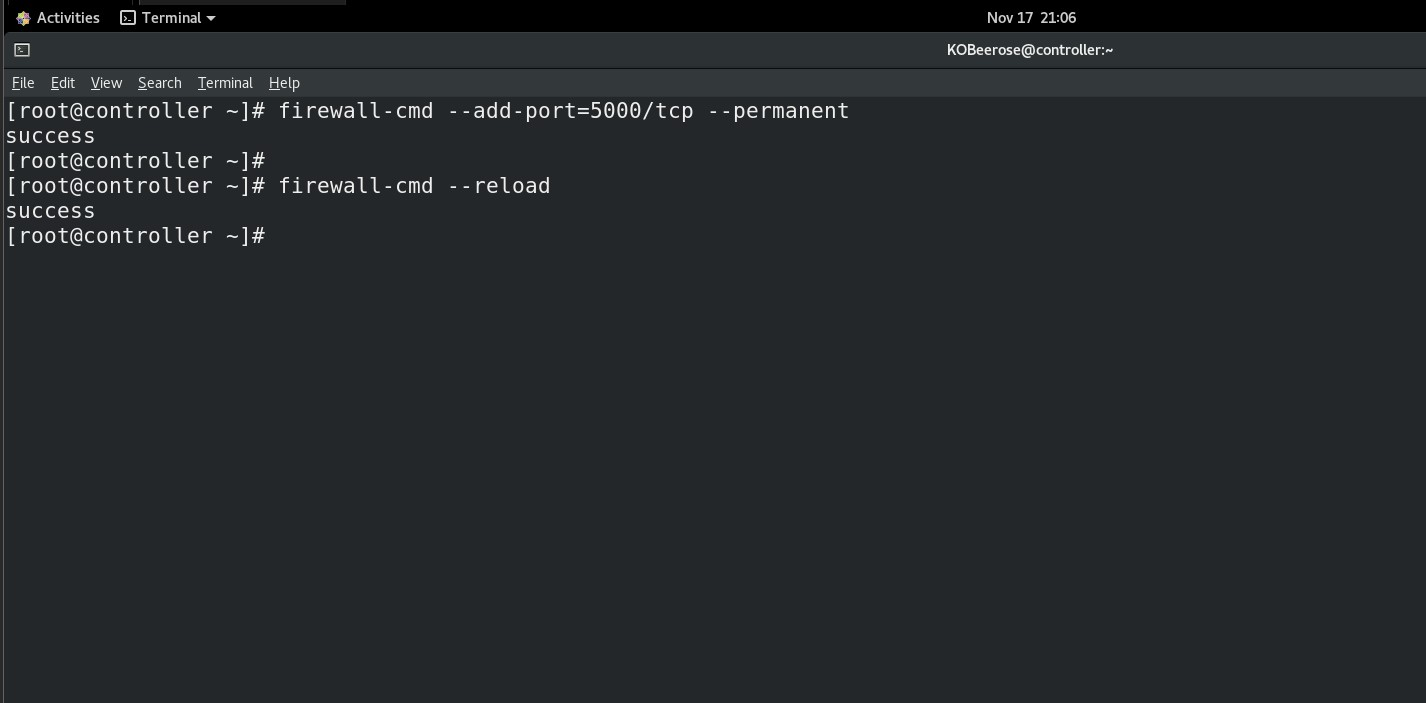
\includegraphics[width=1\linewidth]{Cloud/Configure Keystone #1/Allowing 5000 port} 
\end{center} 
\caption{Allowing 5000 port} 
\end{figure}  \FloatBarrier
\\
\par 
Once everything is configured, we will modify the /etc/httpd/conf/httpd.conf file to set the server name, then start Apache httpd. 
\\
\begin{figure}[!htb] 
\begin{center} 
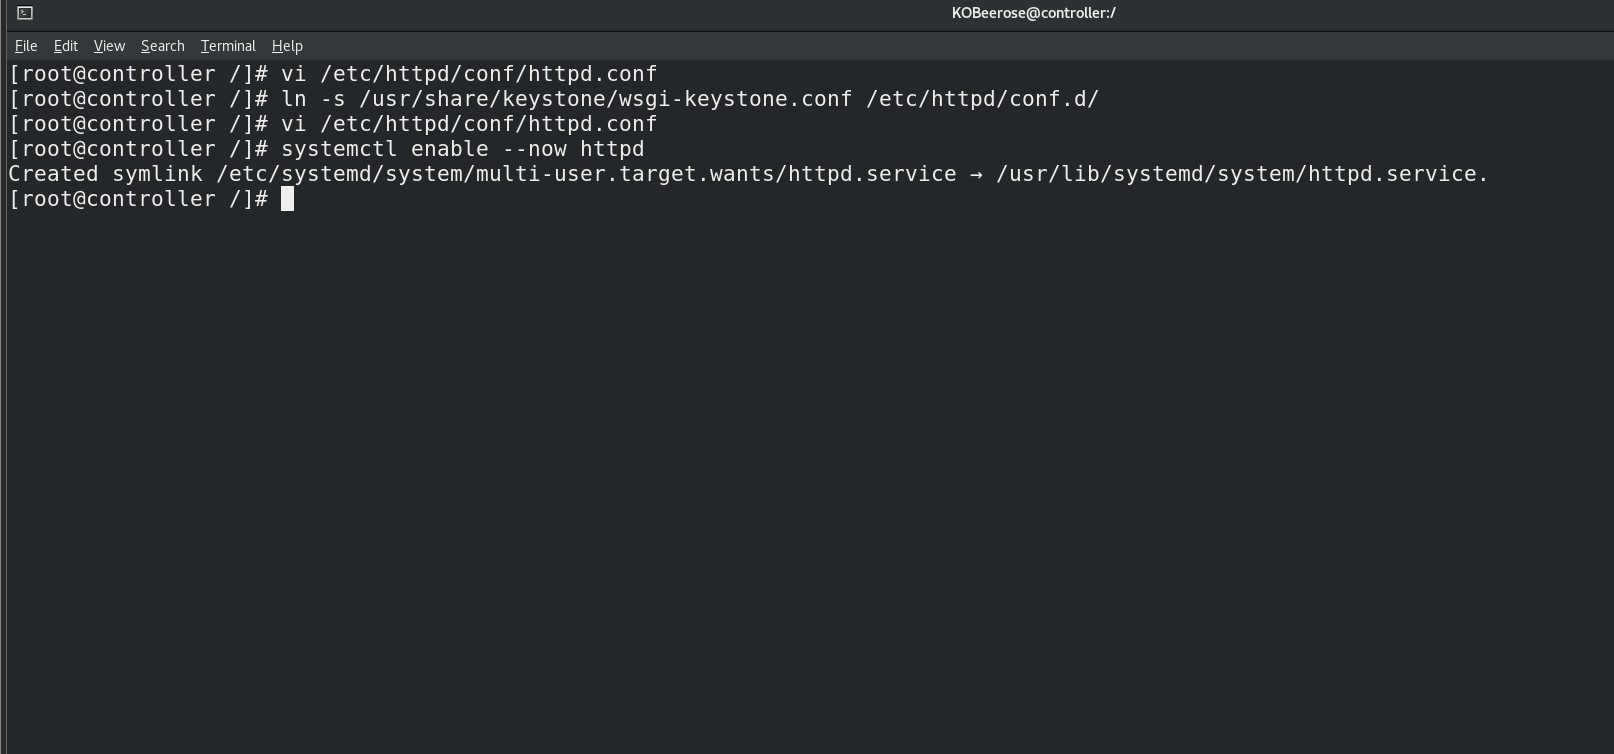
\includegraphics[width=1\linewidth]{Cloud/Configure Keystone #1/Apache httpd} 
\end{center} 
\caption{Apache httpd} 
\end{figure}  \FloatBarrier
\\
\section{Creating and Load environment variables file}

\par One more step before creating keystone projects, we are going to export some environment variables written in the  / keystonerc file as shown below: 
\begin{figure}[!htb] 
\begin{center} 
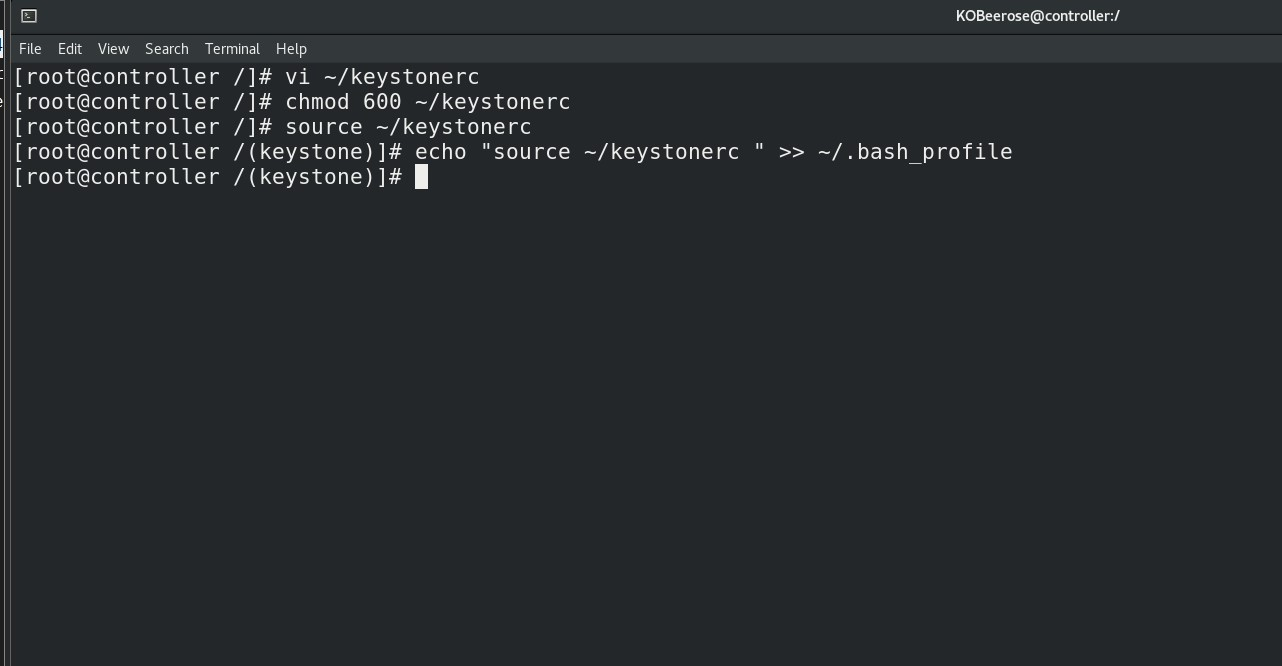
\includegraphics[width=0.94\linewidth]{Cloud/Configure Keystone #2/Creating env var file} 
\end{center} 
\caption{Creating env var file} 
\end{figure}  \FloatBarrier

\section{Creating Projects}

\par Finally, we can create a service project named service. to check it, we can display all the created projects 

\begin{figure}[!htb] 
\begin{center} 
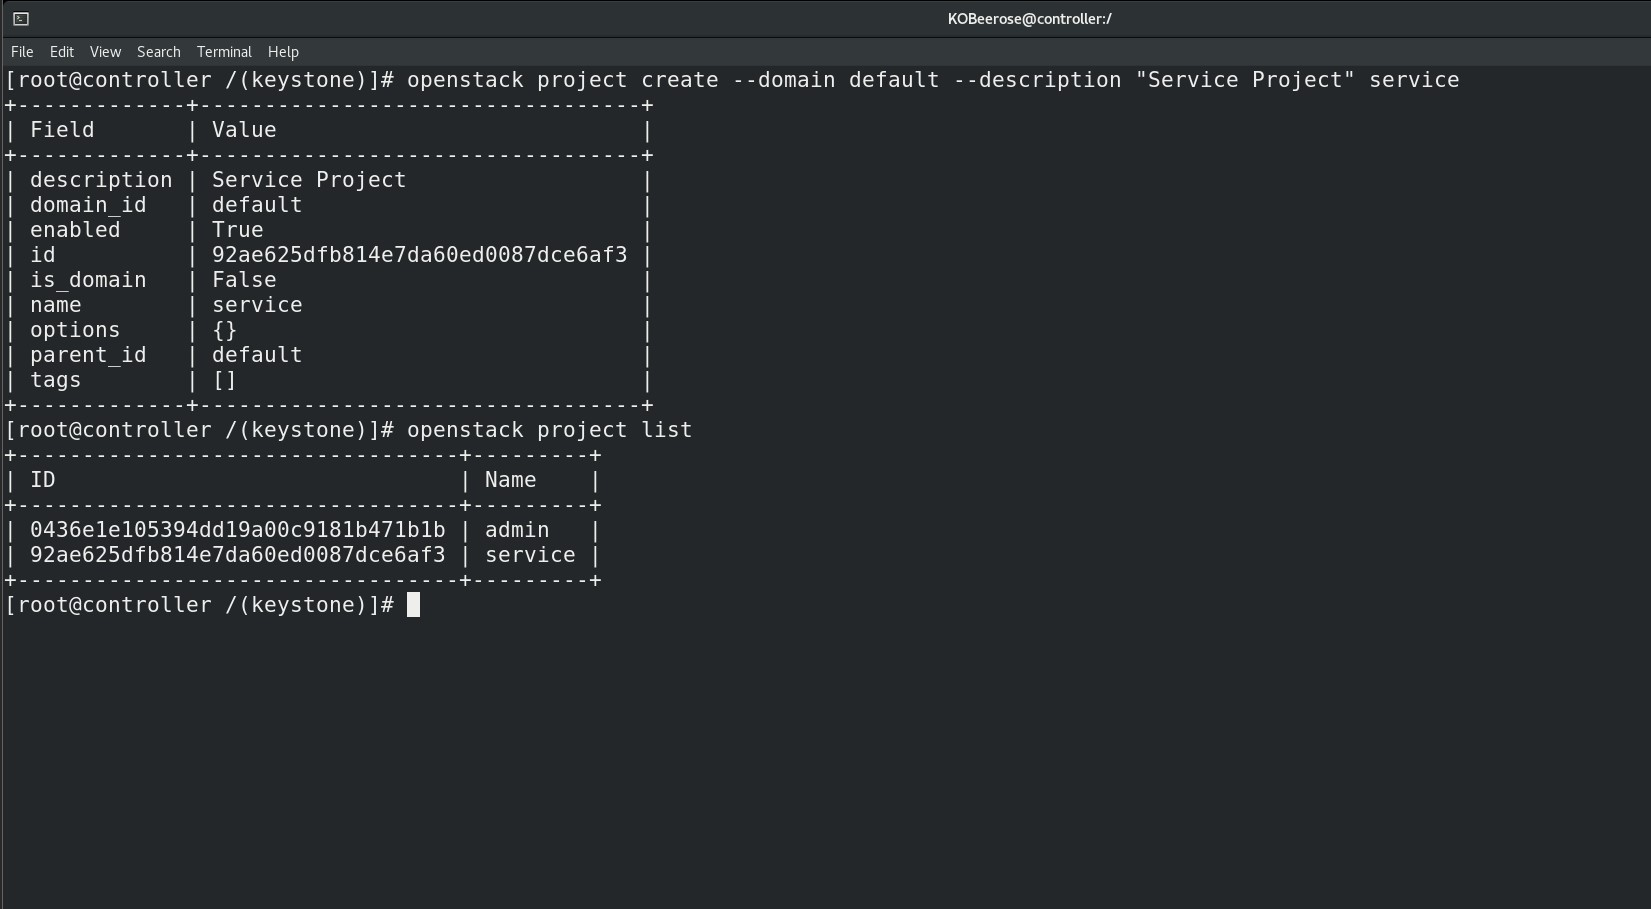
\includegraphics[width=.94\linewidth]{Cloud/Configure Keystone #2/Create Project} 
\end{center} 
\caption{Create Project} 
\end{figure}  \FloatBarrier
\\

\end{spacing}

\chapter{Running Map/Reduce in a multi-node cluster}
\par In this section we will running a Map / Reduce program in a multi-node cluster.
%Intro\footnotemark\\
\begin{spacing}{1.2}
%note en bas de page
\section{Checking all the nodes of the cluster}

\par Let's verify the good functioning of all the nodes of the cluster.
\\
\begin{figure}[!htb] 
\begin{center} 
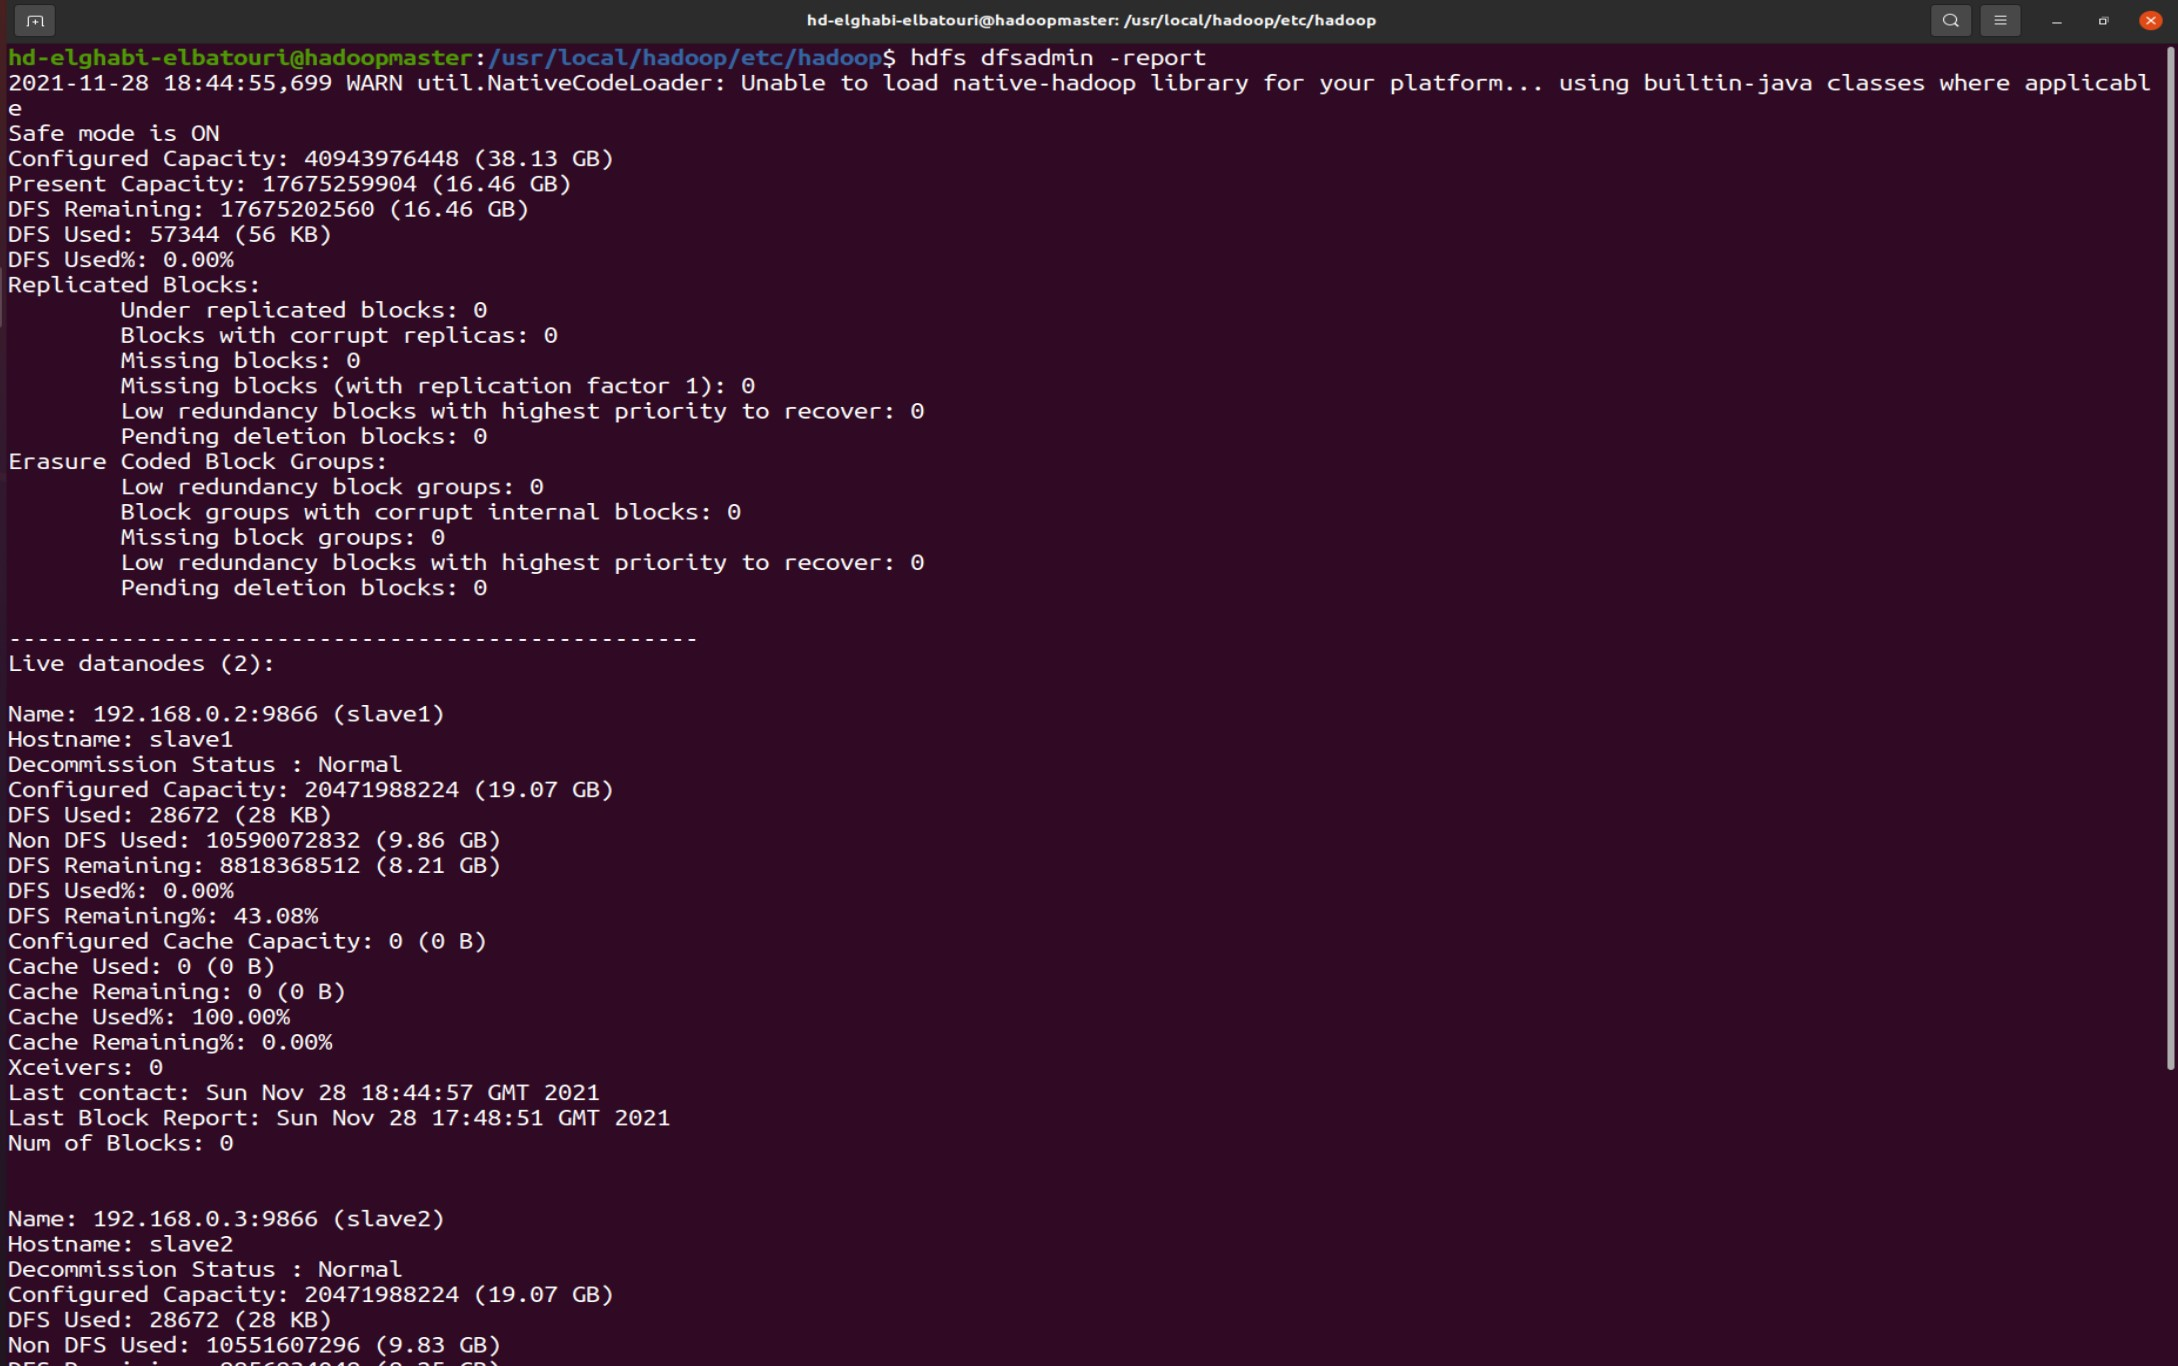
\includegraphics[width=1\linewidth]{Big_Data/Hadoop/Multi-Nodes Map_Reduce/Verifying cluster nodes.jpg} 
\end{center} 
\caption{caption} 
\end{figure} 
\FloatBarrier



\section{Executing Map/Reduce}

\par thisIsAveryLongParagraphToUseAsAtemplateForCopyAndPastingContentInAgoodWay
\\
\begin{figure}[!htb] 
\begin{center} 
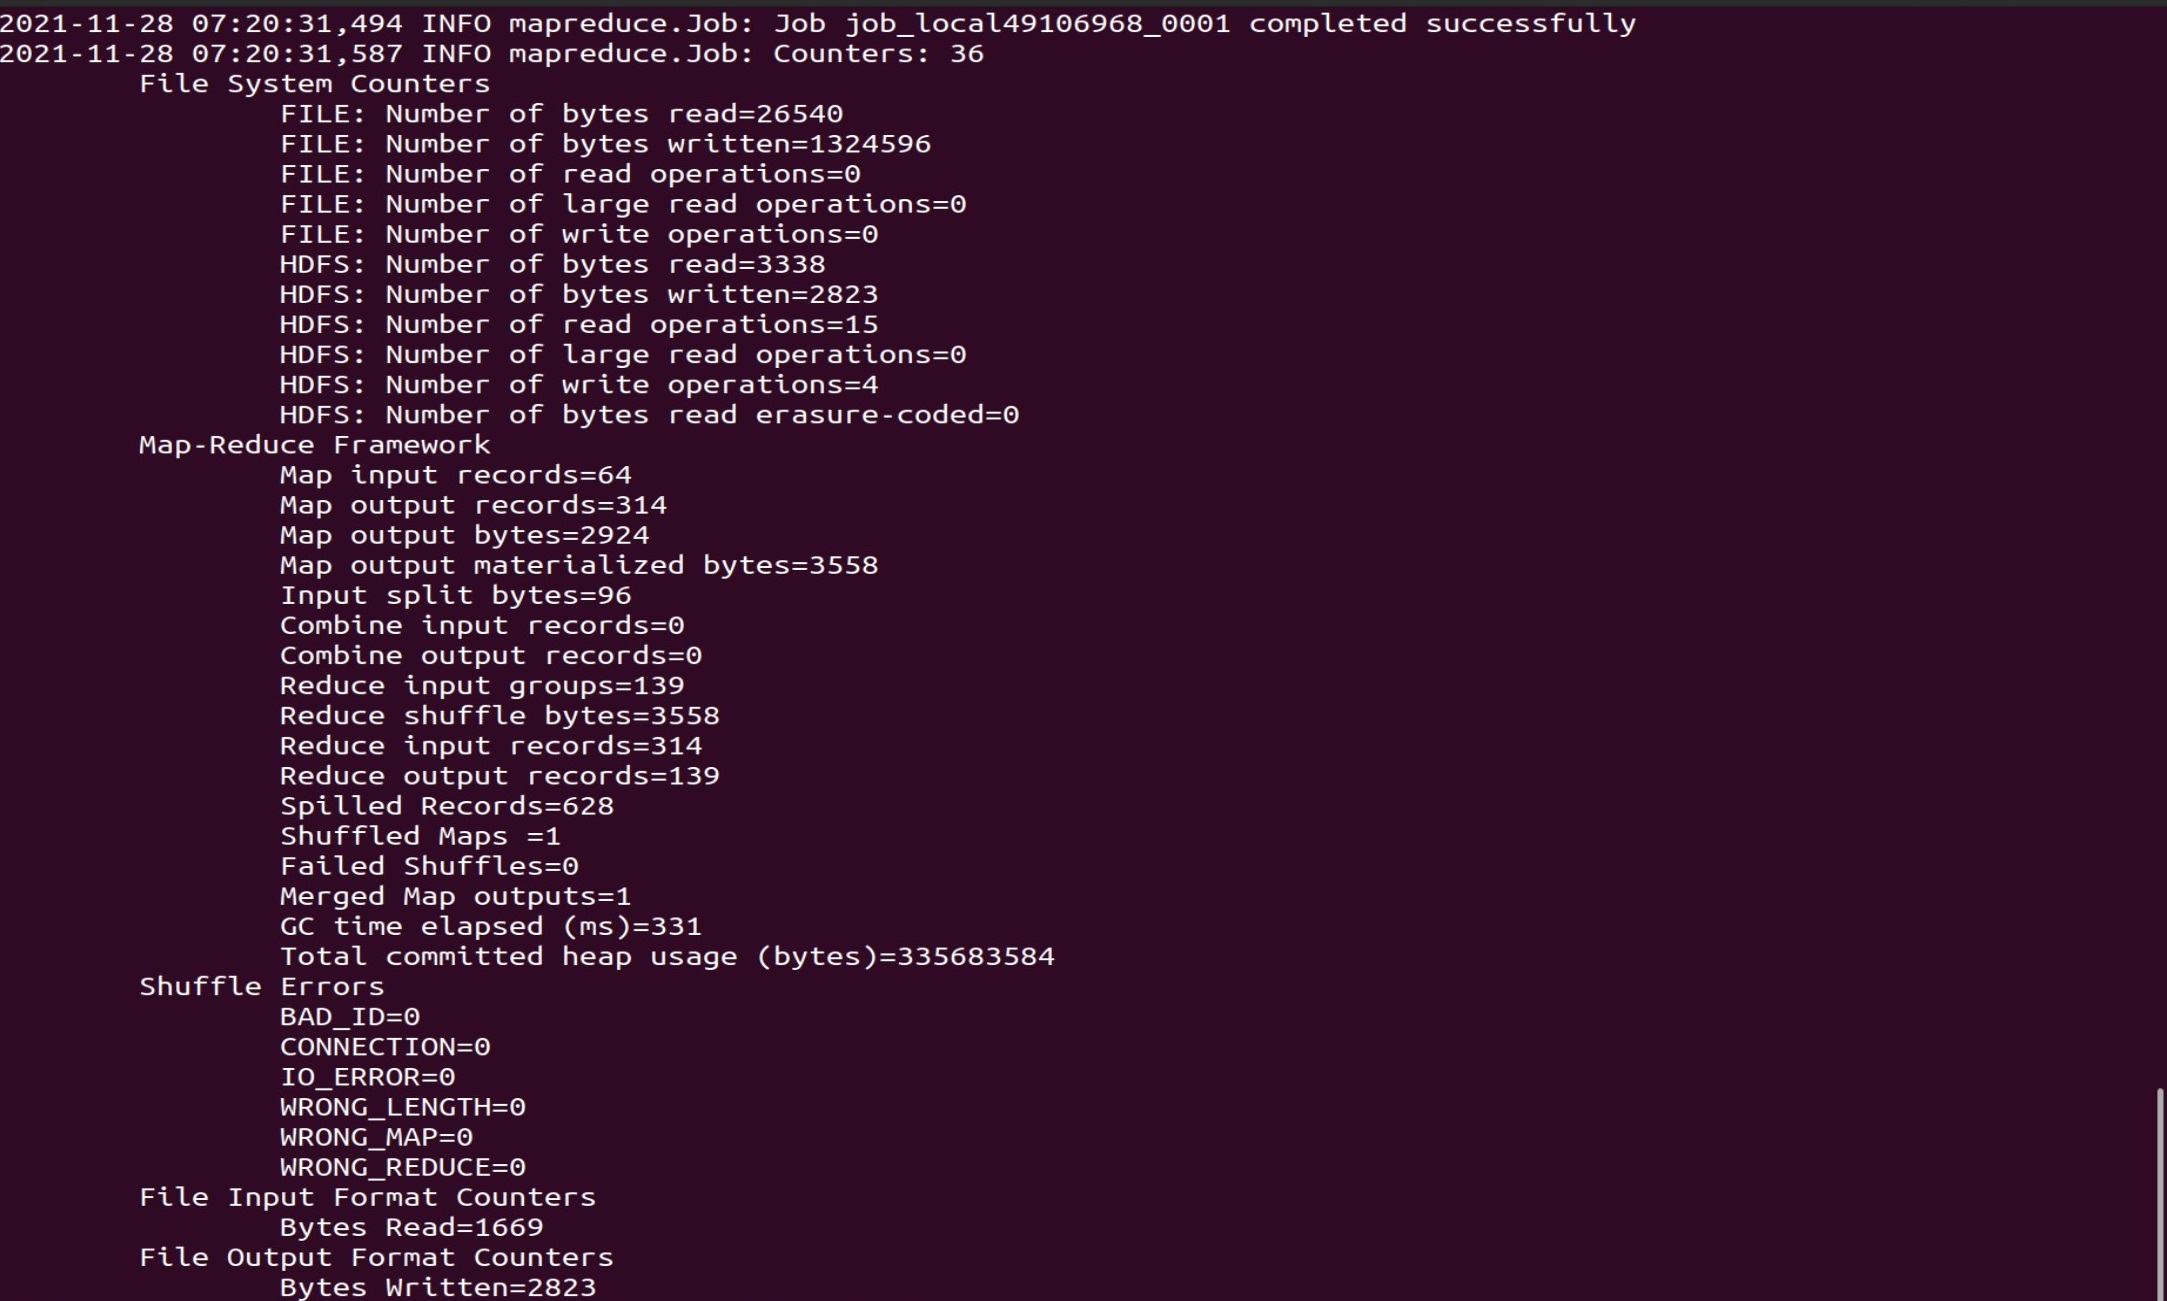
\includegraphics[width=1\linewidth]{Big_Data/Hadoop/Multi-Nodes Map_Reduce/running wordcount.jpg} 
\end{center} 
\caption{caption} 
\end{figure} 
\FloatBarrier


\section{Showing results}

\par Getting the result of the Map / Reduce algorithm.
\\
\begin{figure}[!htb] 
\begin{center} 
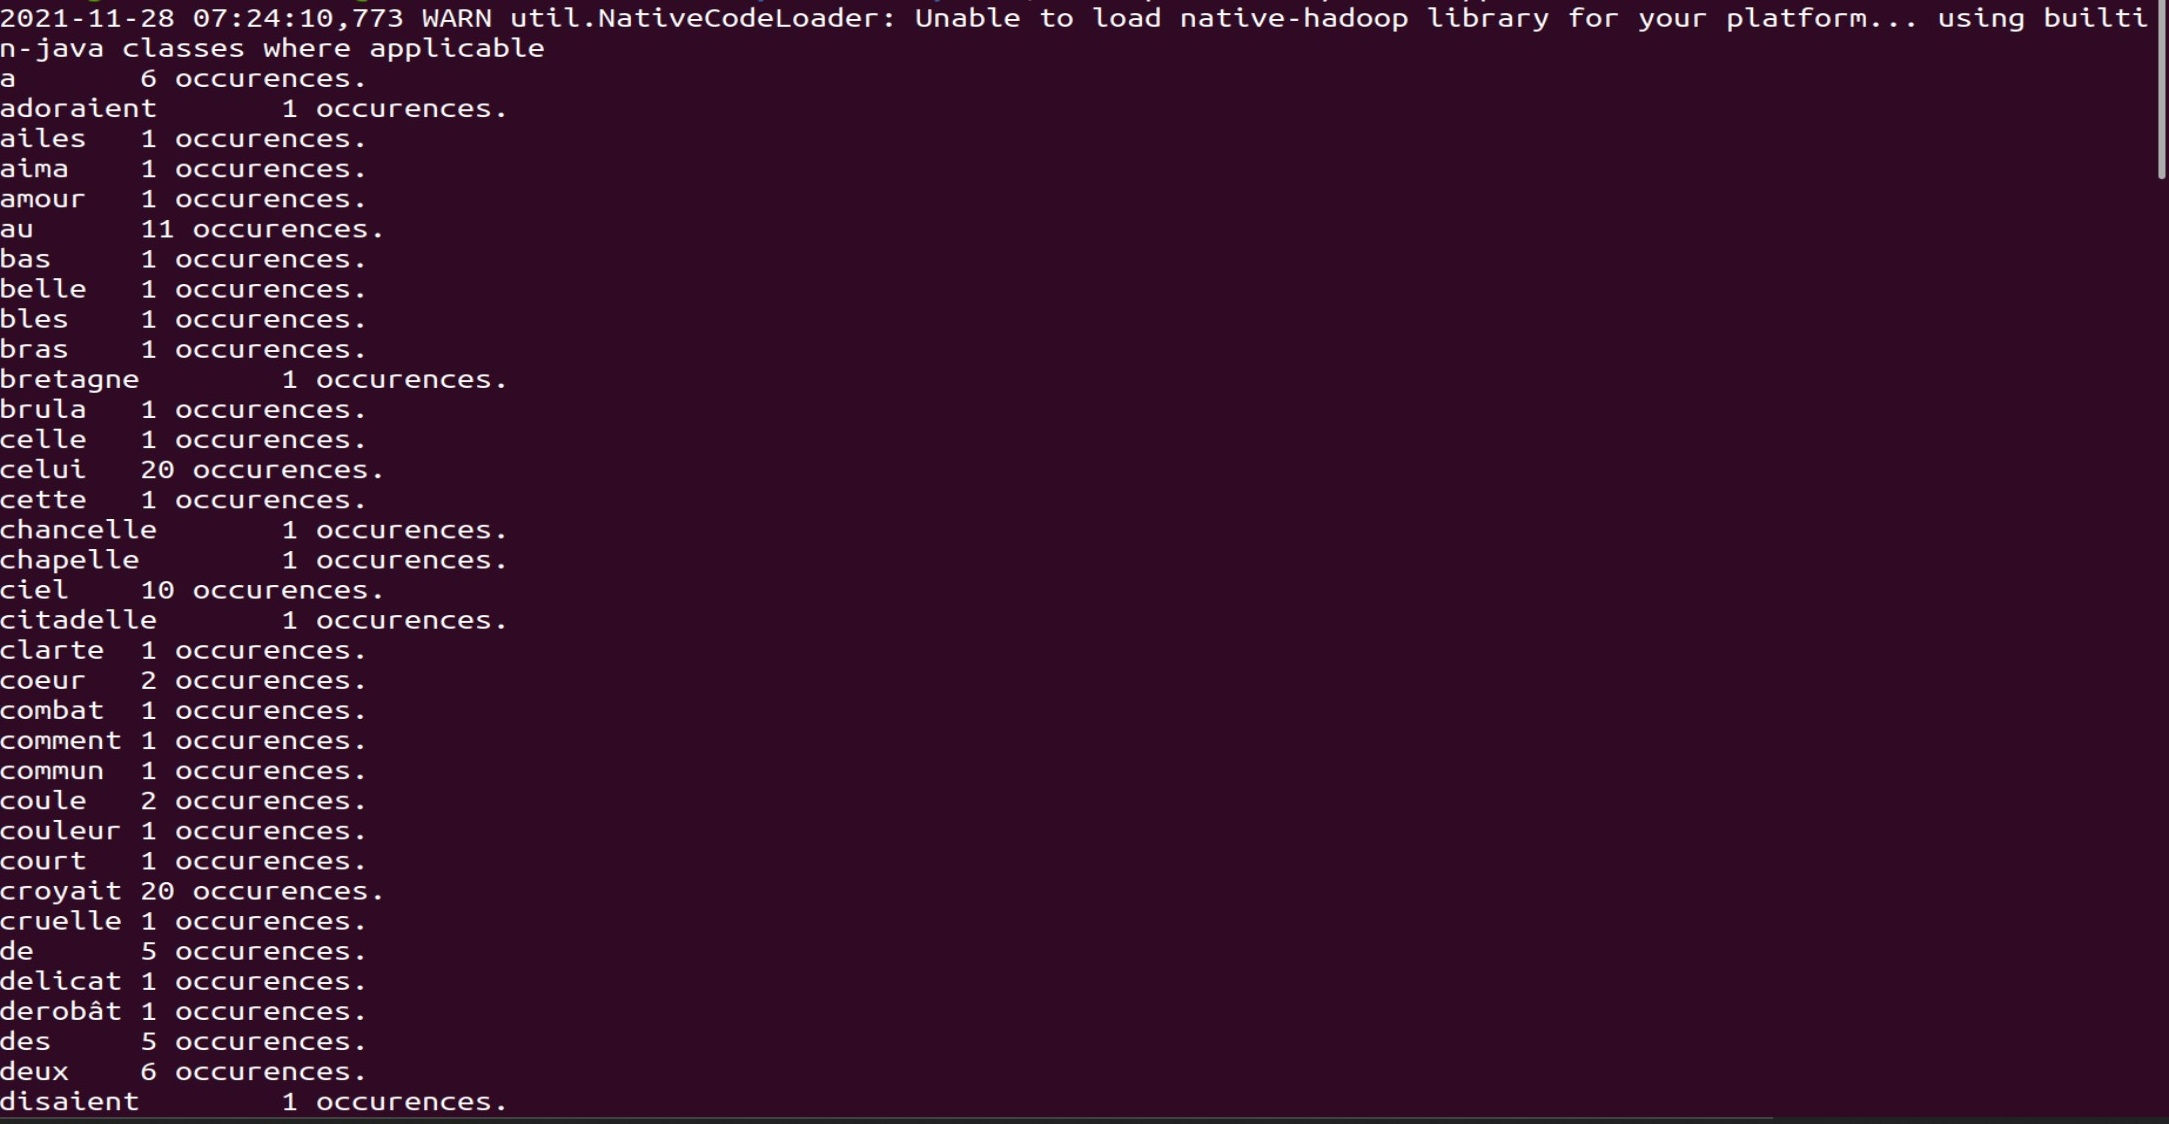
\includegraphics[width=1\linewidth]{Big_Data/Hadoop/Multi-Nodes Map_Reduce/Showing results.jpg} 
\end{center} 
\caption{caption} 
\end{figure} 
\FloatBarrier


\end{spacing}

\chapter{Installing and configuring Spark locally}
\par In this section we are going to use Spark locally on the ubuntu VM created previously. We will run
Spark on Hadoop YARN. YARN will thus take care of the management of resources for the triggering and
execution of Spark Jobs. 
%Intro\footnotemark\\
\begin{spacing}{1.2}
%note en bas de page
\section{Downloading and Extracting files}

\par Let's start as always by checking the status of the machine
\\
\begin{figure}[!htb] 
\begin{center} 
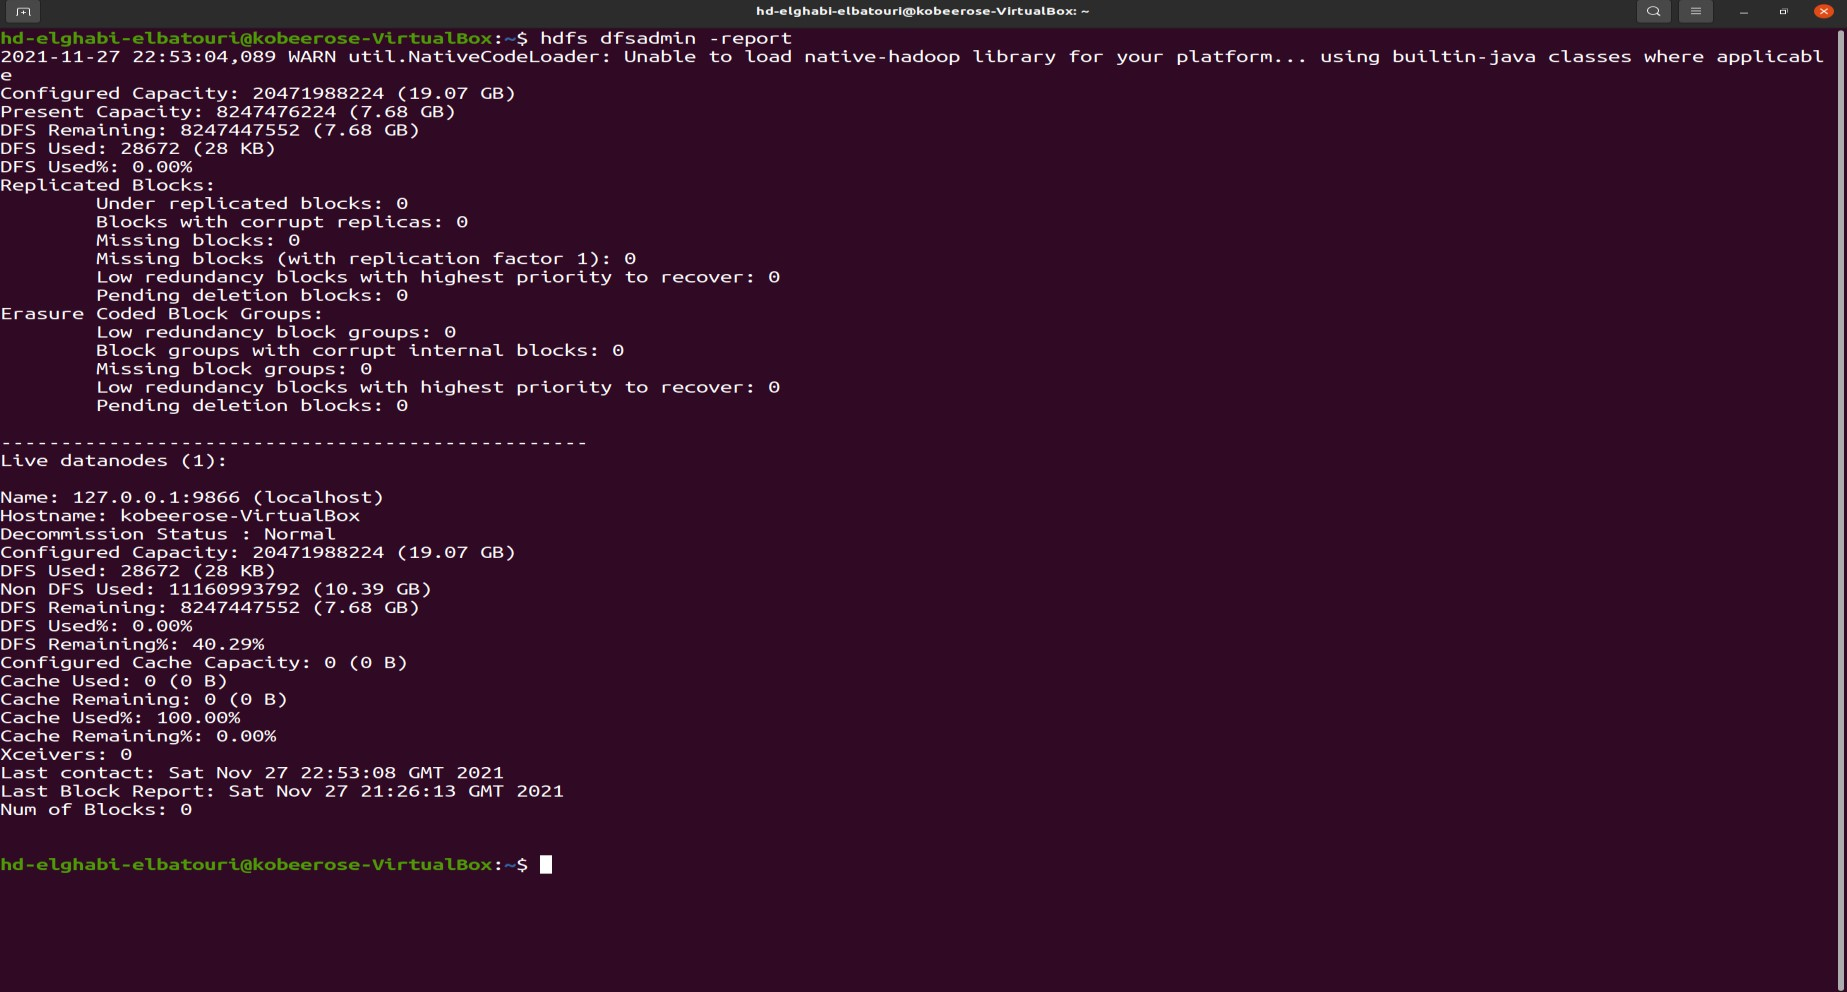
\includegraphics[width=1\linewidth]{Big_Data/Spark/Spark Installation & Configuration/Live datanode} 
\end{center} 
\caption{Live datanode} 
\end{figure} 
\FloatBarrier



\par After downloading the source files, we will extract them in the download folder.
\\
\begin{figure}[!htb] 
\begin{center} 
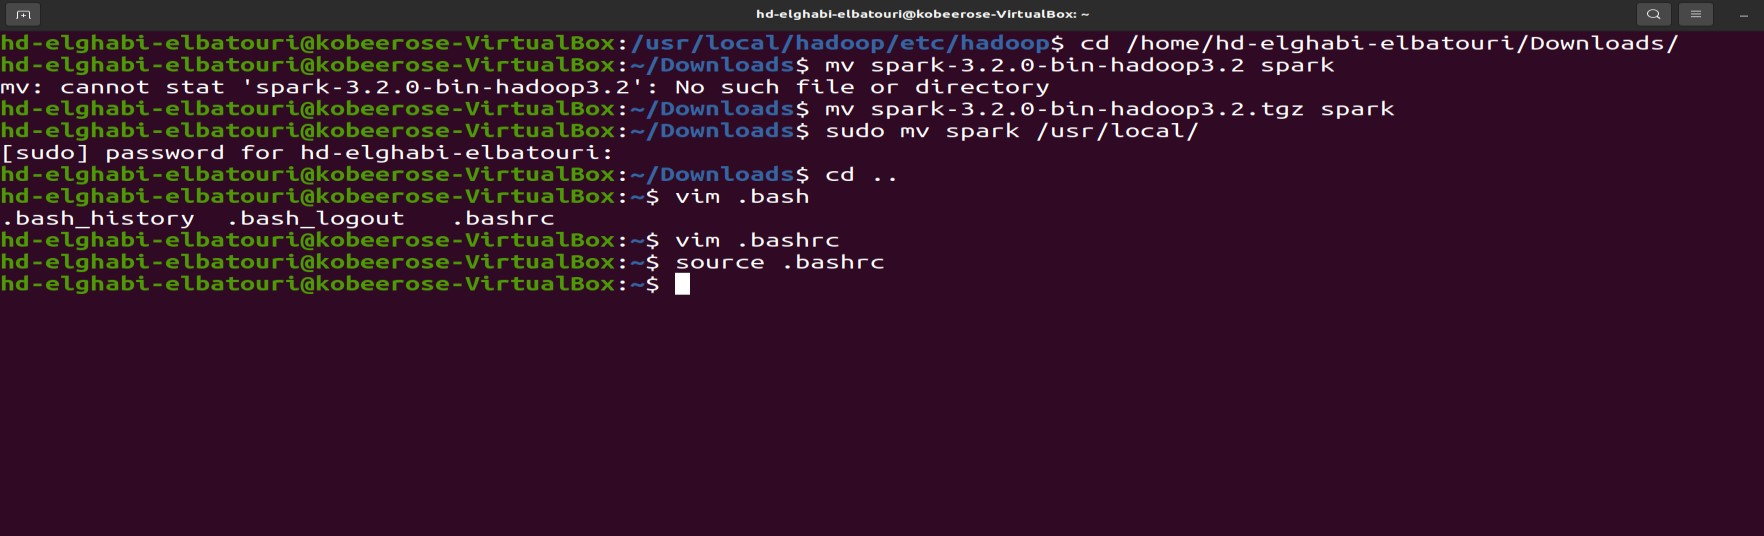
\includegraphics[width=1\linewidth]{Big_Data/Spark/Spark Installation & Configuration/Extracting Spark} 
\end{center} 
\caption{Extracting Spark} 
\end{figure} 
\FloatBarrier

\section{Configure the PATH in the .bashrc}

\par modify the PATH by adding the path where the bin of spark exists.
\\
\begin{figure}[!htb] 
\begin{center} 
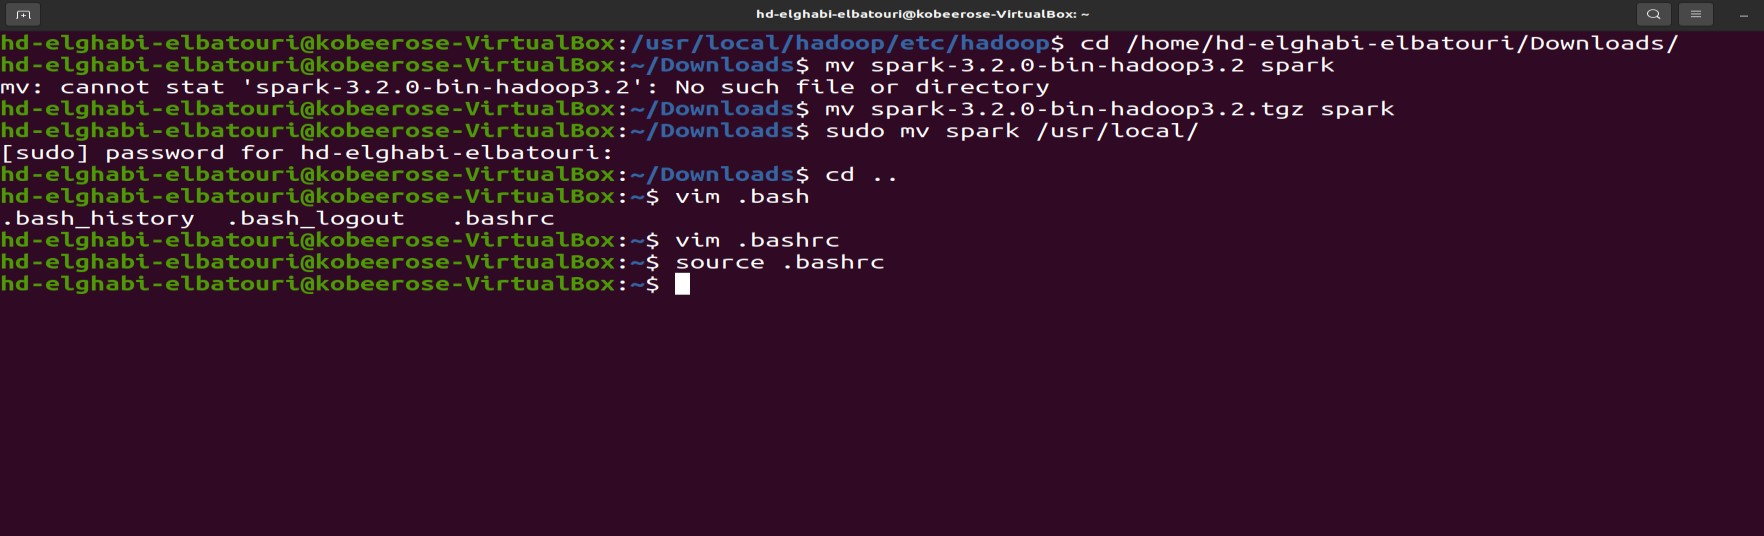
\includegraphics[width=1\linewidth]{Big_Data/Spark/Spark Installation & Configuration/.bashrc config} 
\end{center} 
\caption{.bashrc config} 
\end{figure} 
\FloatBarrier

\section{Installing Python}


\par Let's install python on our machine.
\\
\begin{figure}[!htb] 
\begin{center} 
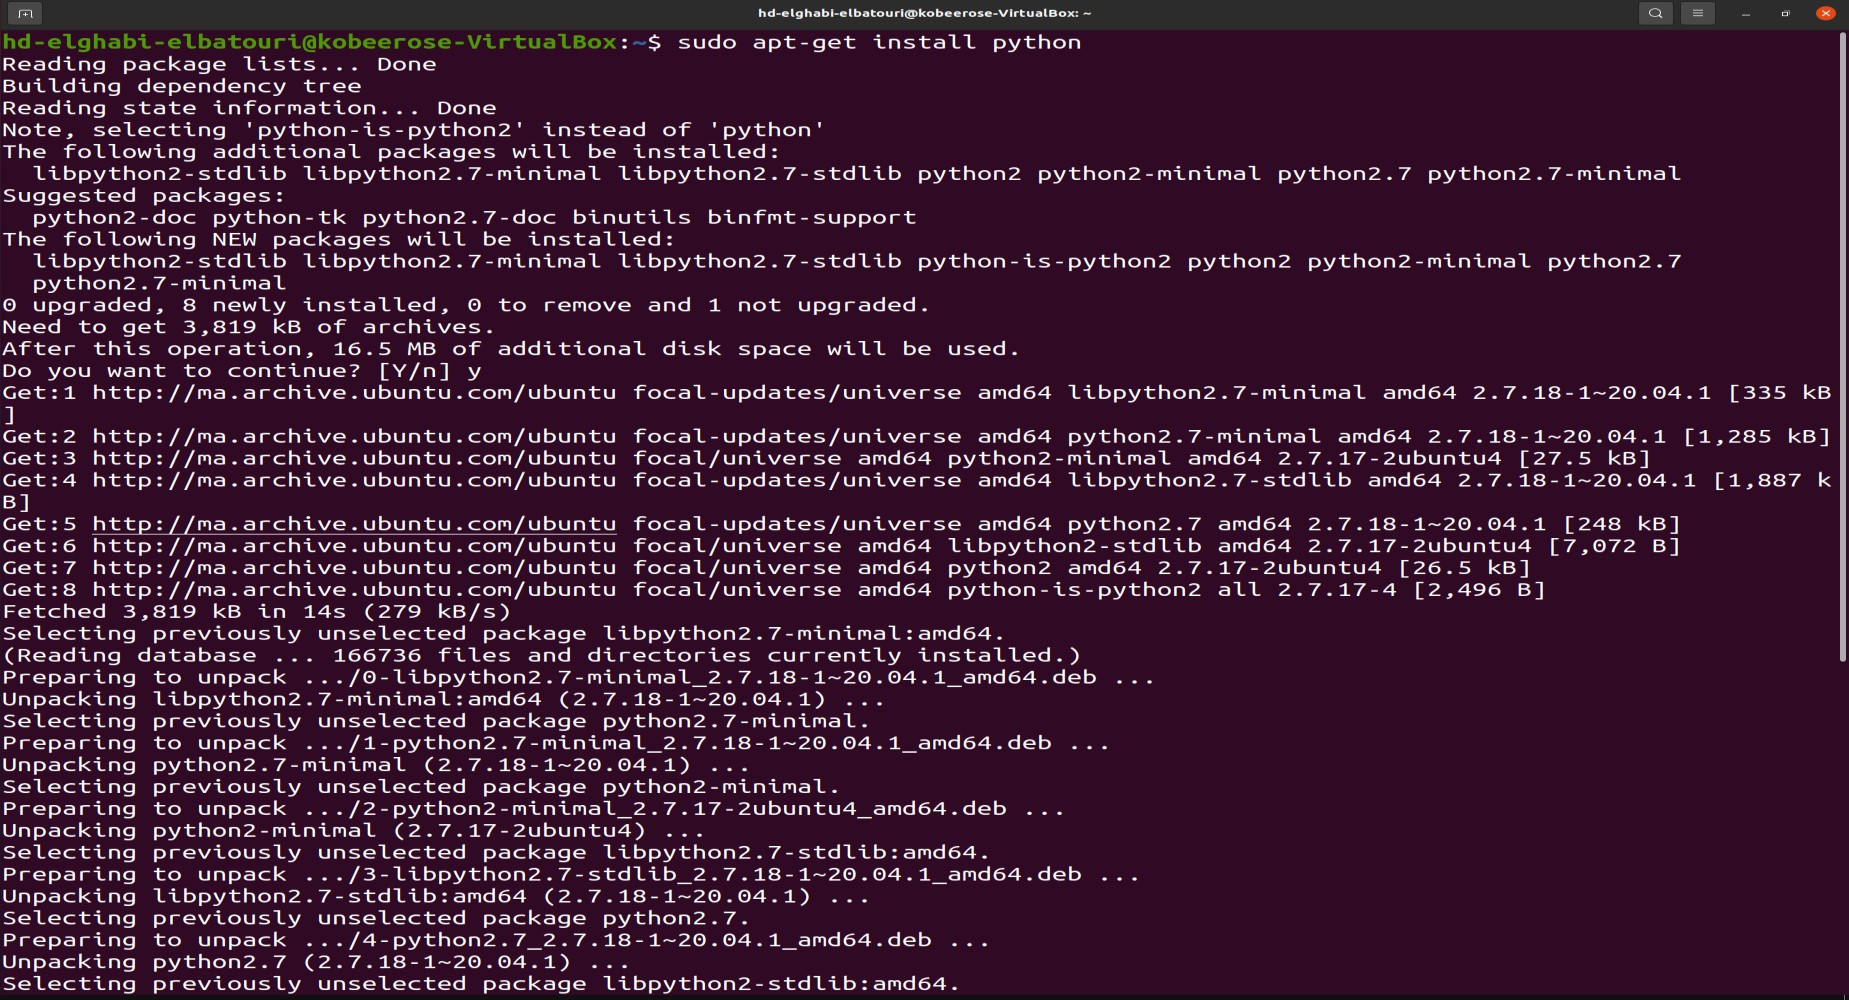
\includegraphics[width=1\linewidth]{Big_Data/Spark/Spark Installation & Configuration/Installing Python} 
\end{center} 
\caption{Installing Python} 
\end{figure} 
\FloatBarrier


\par Accessing the Python terminal for Spark.
\\
\begin{figure}[!htb] 
\begin{center} 
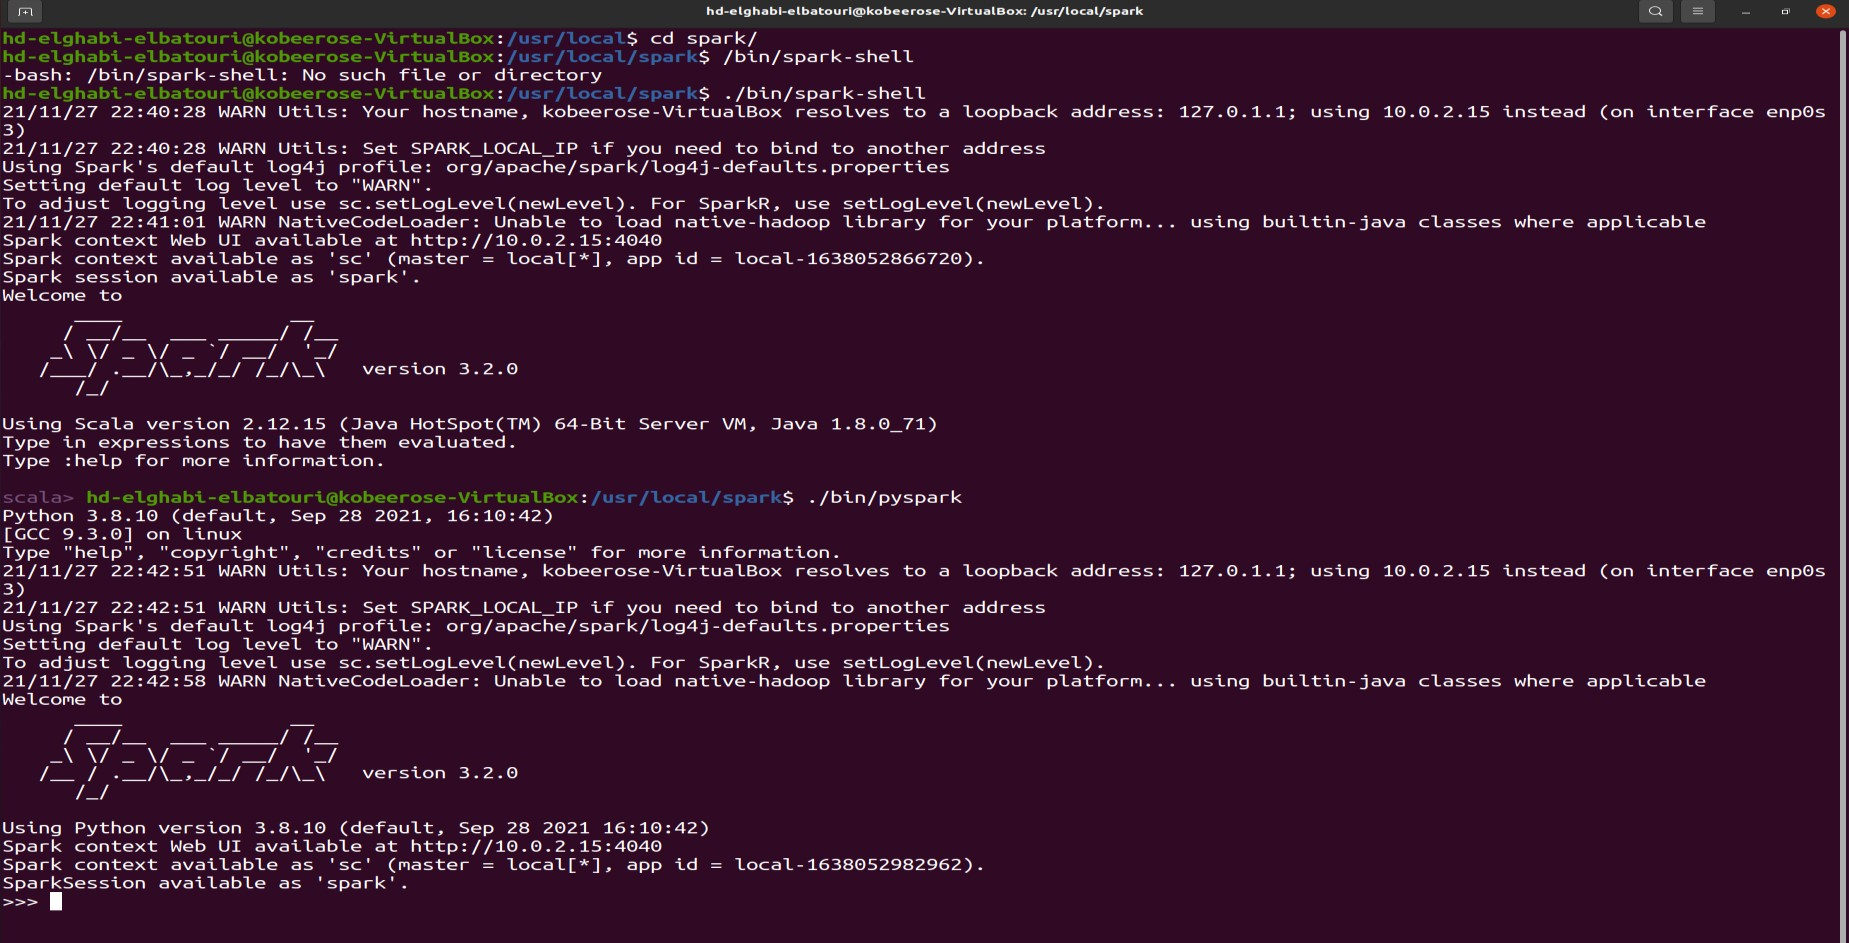
\includegraphics[width=1\linewidth]{Big_Data/Spark/Spark Installation & Configuration/spark-shell & pyspark} 
\end{center} 


\chapter{Nova Configuration}
\par In this section, we will install and configure OpenStack Compute Service (Nova).
%Intro\footnotemark\\
\begin{spacing}{1.2}
%note en bas de page
\section{Nova Setup in Keystone}
\subsection{Adding users for Nova in Keystone}

\\
\par We will start by creating a new nova user in the project department. 
\begin{figure}[!htb] 
\begin{center} 
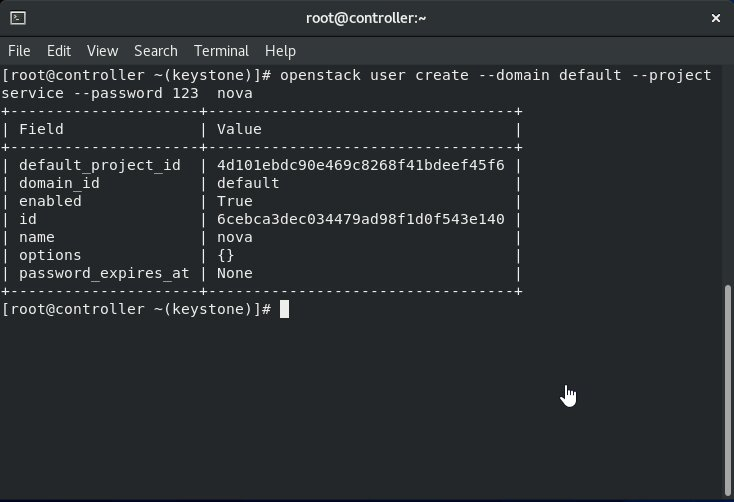
\includegraphics[width=1\linewidth]{Cloud/Nova Setup in Keystone/Create [Nova] User In [Service] Project} 
\end{center} 
\caption{Create [Nova] User In [Service] Project} 
\end{figure}  \FloatBarrier 
\\
\begin{figure}[!htb] 
\begin{center} 
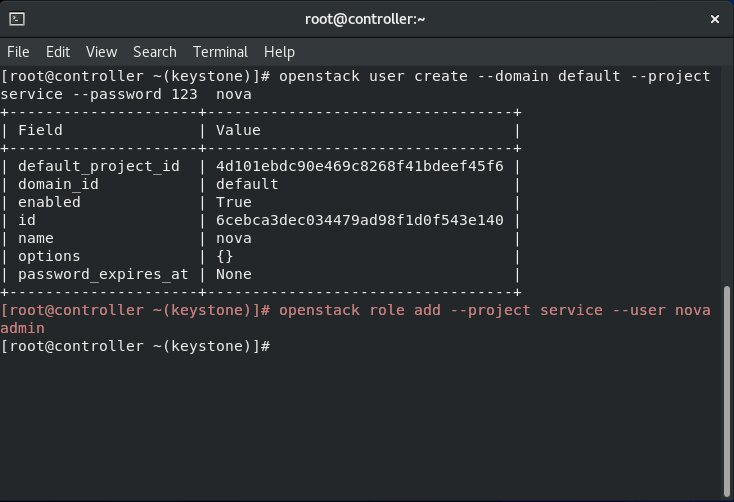
\includegraphics[width=1\linewidth]{Cloud/Nova Setup in Keystone/Add [Nova] User In [Admin] Role} 
\end{center} 
\caption{Add [Nova] User In [Admin] Role} 
\end{figure}  \FloatBarrier 
\\

\section{Installing Keystone}

\par Next, we will assign this new user the role of administrator. Likewise, we
let's create a user of type placement and also give him the role of administrator. 
\\
\begin{figure}[!htb] 
\begin{center} 
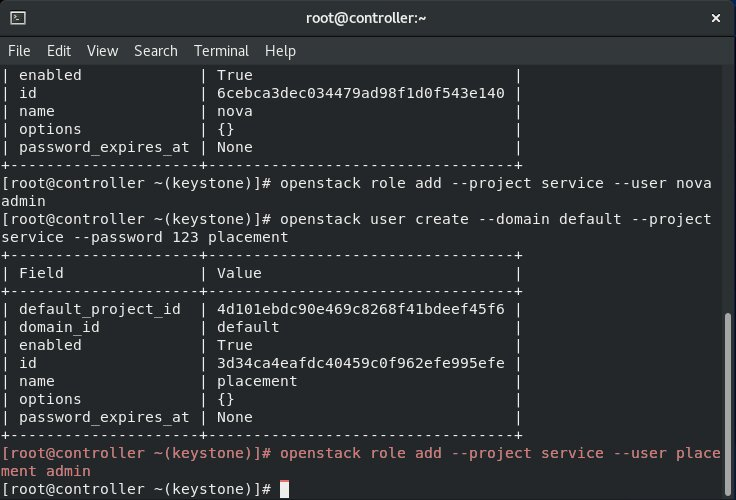
\includegraphics[width=1\linewidth]{Cloud/Nova Setup in Keystone/Add [Placement] User In [Admin] Role}
\end{center} 
\caption{Add [Placement] User In [Admin] Role} 
\end{figure}  \FloatBarrier 
\\
\par Now we are going to create a service entry for nova and another for placement. 
\begin{figure}[!htb] 
\begin{center} 
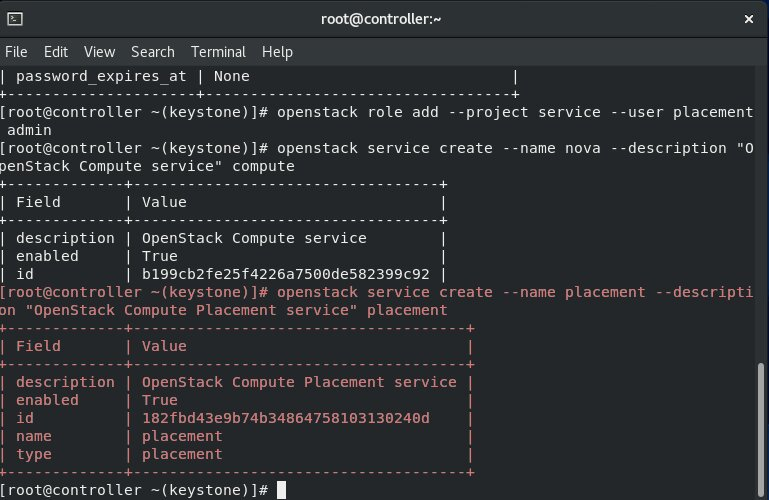
\includegraphics[width=1\linewidth]{Cloud/Nova Setup in Keystone/Create Service Entry For [Placement]} 
\end{center} 
\caption{Create Service Entry For [Placement]} 
\end{figure}  \FloatBarrier 
\\

\par We must define the nova API as host and create an endpoint for nova and placement in interfaces
public, internal and admin  .\\

\\
\begin{figure}[!htb] 
\begin{center} 
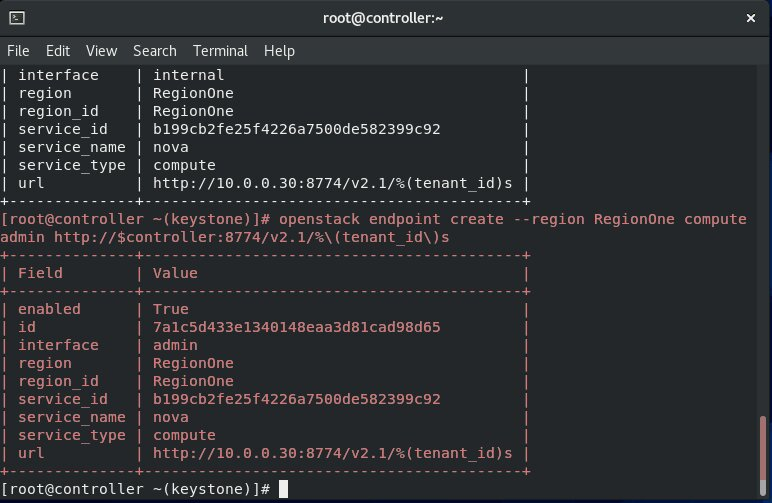
\includegraphics[width=1\linewidth]{Cloud/Nova Setup in Keystone/Create Endpoint For [Nova] (Admin)} 
\end{center} 
\caption{Create Endpoint For [Nova] (Admin)} 
\end{figure}  \FloatBarrier 
\\
\\
\begin{figure}[!htb] 
\begin{center} 
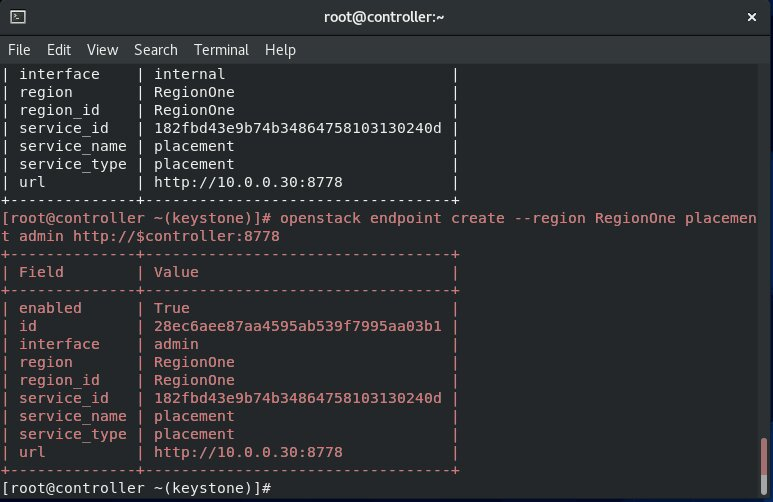
\includegraphics[width=1\linewidth]{Cloud/Nova Setup in Keystone/Create Endpoint For [Placement] (Admin)} 
\end{center} 
\caption{Create Endpoint For [Placement] (Admin)} 
\end{figure}  \FloatBarrier 
\\
\subsection{Adding a Database on MariaDB for Nova}
\par We will then add the nova, placement, nova api and nova cell0 databases to our Mariadb. 
\\
\begin{figure}[!htb] 
\begin{center} 
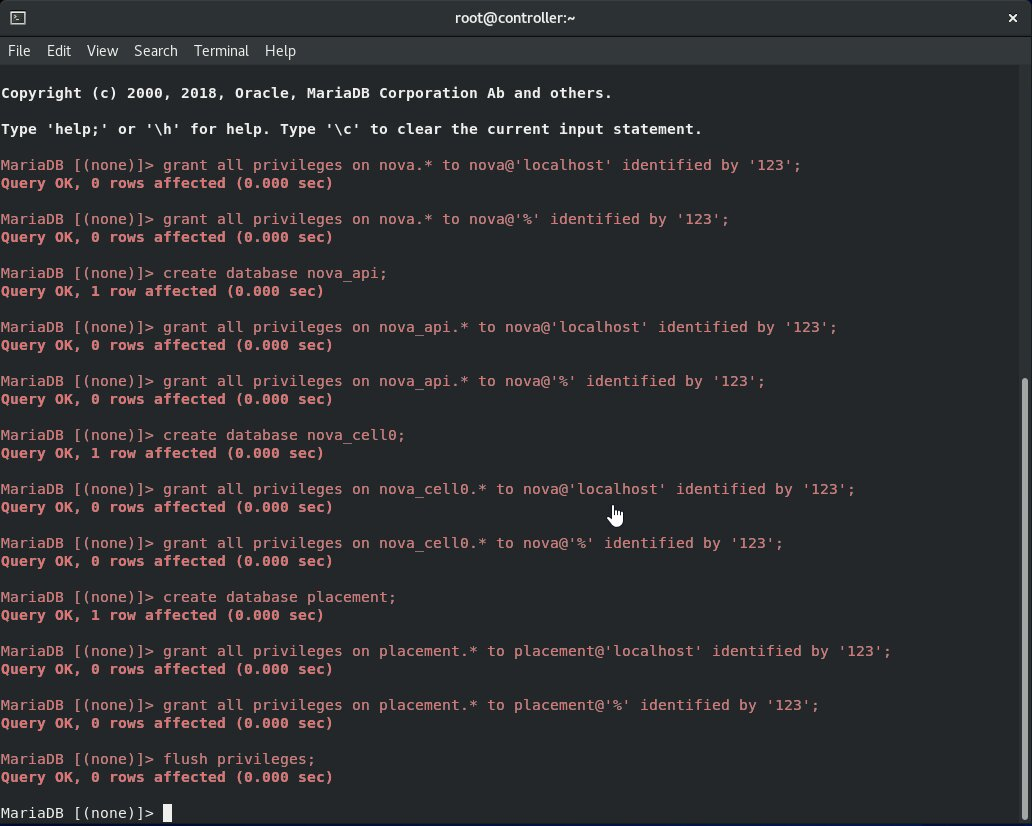
\includegraphics[width=1\linewidth]{Cloud/Nova Setup in Keystone/Add A User And Database On Mariadb For Nova} 
\end{center} 
\caption{Add A User And Database On Mariadb For Nova} 
\end{figure}  \FloatBarrier 
\\

\section{Installing and Configuring Nova services}
\subsection{Installing Nova services}
\par 
Now it's time to install Nova services and then configure it. 
\\
\begin{figure}[!htb] 
\begin{center} 
\includegraphics[width=1\linewidth]{Cloud/Installing and Configuring Nova services/Installing Nova services} 
\end{center} 
\caption{Installing Nova services} 
\end{figure}  \FloatBarrier 
\\

\subsection{Configuring Nova}
\par 
For the configuration, we will rename the file etc/nova/nova.conf.org in
Etc/nova/nova.conf.\newline Here is the contents of the file: 
\\
\begin{figure}[!htb] 
\begin{center} 
\includegraphics[width=1\linewidth]{Cloud/Installing and Configuring Nova services/Creating nova.conf} 
\end{center} 
\caption{Creating nova.conf} 
\end{figure}  \FloatBarrier 
\\

\par 
We are going to change the access permissions to this file with the chmod 640 command which means
that the owner has read and write rights, that the group has read-only rights and that
all other users have no rights to the file.
\\
\begin{figure}[!htb] 
\begin{center} 
\includegraphics[width=1\linewidth]{Cloud/Installing and Configuring Nova services/nova.conf access} 
\end{center} 
\caption{nova.conf access} 
\end{figure}  \FloatBarrier 
\\


\par now we do the same thing for the placement.conf file
\\
\begin{figure}[!htb] 
\begin{center} 
\includegraphics[width=1\linewidth]{Cloud/Installing and Configuring Nova services/Creating placement.conf} 
\end{center} 
\caption{Creating placement.conf} 
\end{figure}  \FloatBarrier 

\\
\begin{figure}[!htb] 
\begin{center} 
\includegraphics[width=1\linewidth]{Cloud/Installing and Configuring Nova services/placement.conf access} 
\end{center} 
\caption{placement.conf access} 
\end{figure}  \FloatBarrier 
\\
\\
\begin{figure}[!htb] 
\begin{center} 
\includegraphics[width=1\linewidth]{Cloud/Installing and Configuring Nova services/Changing 00-placement-api.conf} 
\end{center} 
\caption{Changing 00-placement-api.conf} 
\end{figure}  \FloatBarrier 
\\
\subsection{novaapi.te config}
\par We will install openstack-selinux using dnf and we will adjust the port to be
tcp 8778. Here is the content of the novaapi.te file 
\\
\subsection{Starting Nova services}
\par We will then chain these commands to change the SELinux policy: 
\\

\begin{figure}[!htb] 
\begin{center} 
\includegraphics[width=1\linewidth]{Cloud/Installing and Configuring Nova services/Add Data into Database} 
\end{center} 
\caption{Add Data into Database} 
\end{figure}  \FloatBarrier 
\\
\par The status of nova-conductor and nova-scheduler are UP: 
\\
\begin{figure}[!htb] 
\begin{center} 
\includegraphics[width=1\linewidth]{Cloud/Installing and Configuring Nova services/Show Compute status} 
\end{center} 
\caption{Show Compute status} 
\end{figure}  \FloatBarrier 
\\
\section{Installing and Configuring Nova Compute}
\subsection{Installing Nova Compute}
\par After installing the KVM hypervisor we will install nova compute.

\\
\begin{figure}[!htb] 
\begin{center} 
\includegraphics[width=1\linewidth]{Cloud/Installing and Configuring Nova Compute/Install Nova Compute} 
\end{center} 
\caption{Install Nova Compute} 
\end{figure} 
\FloatBarrier
\\
\subsection{nova.conf config}
\par In addition to basic settings of Nova, we will add the following settings to the nova.conf file in order to enable VNC.
\\
\begin{figure}[!htb] 
\begin{center} 
\includegraphics[width=1\linewidth]{Cloud/Installing and Configuring Nova Compute/Add Follows (Enable Vnc)} 
\end{center} 
\caption{Add Follows (Enable Vnc)} 
\end{figure} 
\FloatBarrier
\\

\subsection{Start Nova Compute}

\par First thing is changing the SELinux policy and enabling openstack-nova-compute,and finally starting the Nova Compute 
\\
\begin{figure}[!htb] 
\begin{center} 
\includegraphics[width=1\linewidth]{Cloud/Installing and Configuring Nova Compute/Start Nova Compute} 
\end{center} 
\caption{Start Nova Compute} 
\end{figure} 
\FloatBarrier
\\
\\
\begin{figure}[!htb] 
\begin{center} 
\includegraphics[width=1\linewidth]{Cloud/Installing and Configuring Nova Compute/Show Status} 
\end{center} 
\caption{Show Status} 
\end{figure} 
\FloatBarrier
\\



\end{spacing}

\chapter{Neutron Configuration}
%Intro\footnotemark\\
\begin{spacing}{1.2}
%note en bas de page
\section{Neutron Setup in Keystone}
\subsection{Adding user or service for Neutron on Keystone}
\par We will start by creating a new Neutron user, assigning him the role of admin,

\\
\begin{figure}[!htb] 
\begin{center} 
\includegraphics[width=1\linewidth]{Cloud/Neutron Setup in Keystone/create [neutron] user in [service] project} 
\end{center} 
\caption{create [neutron] user in [service] project} 
\end{figure} 
\FloatBarrier
\\
\begin{figure}[!htb] 
\begin{center} 
\includegraphics[width=1\linewidth]{Cloud/Neutron Setup in Keystone/add [neutron] user in [admin] role}
\end{center} 
\caption{add [neutron] user in [admin] role} 
\end{figure} 
\FloatBarrier

\par creating a service entry for it, define Neutron API as a host.
\\
\begin{figure}[!htb] 
\begin{center} 
\includegraphics[width=1\linewidth]{Cloud/Neutron Setup in Keystone/define Neutron API Host} 
\end{center} 
\caption{define Neutron API Host} 
\end{figure} 
\FloatBarrier

\par creating an endpoint for the interfaces
public, internal and admin, in order to expose neutron services to our different types of users: 
\\
\begin{figure}[!htb] 
\begin{center} 
\includegraphics[width=1\linewidth]{Cloud/Neutron Setup in Keystone/create endpoint for [neutron] (admin)} 
\end{center} 
\caption{create endpoint for [neutron] (admin)} 
\end{figure} 
\FloatBarrier

\subsection{Adding a User and Database on MariaDB for Neutron}
\par Next, we'll add this new user to our mariadb database: 
\\
\begin{figure}[!htb] 
\begin{center} 
\includegraphics[width=1\linewidth]{Cloud/Neutron Setup in Keystone/Add a User and Database on MariaDB for Neutron} 
\end{center} 
\caption{Add a User and Database on MariaDB for Neutron} 
\end{figure} 
\FloatBarrier


\section{Installing and Configuring Neutron services}
\subsection{Installing Neutron services}

\par Now we will install the services of Neutron to configure them later 
\\
\begin{figure}[!htb] 
\begin{center} 
\includegraphics[width=1\linewidth]{Cloud/Installing and Configuring Neutron services/Install Neutron Services 1} 
\end{center} 
\caption{Install Neutron Services 1} 
\end{figure} 
\FloatBarrier
\\

\subsection{Configuring Neutron services}
\par For the configuration, we will rename the file /etc/neutron/neutron.conf.org in \newline
/Etc/neutron/neutron.conf. Here is the contents of the file: 
\\
\begin{figure}[!htb] 
\begin{center} 
\includegraphics[width=1\linewidth]{Cloud/Installing and Configuring Neutron services/Creating neutron.conf} 
\end{center} 
\caption{Creating neutron.conf} 
\end{figure} 
\FloatBarrier
\\
\par We will change the access permissions to this file with the chmod 640 command. Then we
let's define neutron as a group user.

\par In the / etc / neutron / l3 agent.ini file, we will add the following lines: 
\\
\begin{figure}[!htb] 
\begin{center} 
\includegraphics[width=1\linewidth]{Cloud/Installing and Configuring Neutron services/Changing l3_agent.ini} 
\end{center} 
\caption{Changing l3 agent.ini} 
\end{figure} 
\FloatBarrier
\\
\par In the / etc / neutron / dhcp agent.ini file, we will add the following lines: 
\\
\begin{figure}[!htb] 
\begin{center} 
\includegraphics[width=1\linewidth]{Cloud/Installing and Configuring Neutron services/Changing dhcp_agent.ini} 
\end{center} 
\caption{Changing dhcp agent.ini} 
\end{figure} 
\FloatBarrier
\\
\par In the / etc / neutron / metadata agent.ini file, we will add the following code: 
\\
\begin{figure}[!htb] 
\begin{center} 
\includegraphics[width=1\linewidth]{Cloud/Installing and Configuring Neutron services/Changing metadata_agent.ini} 
\end{center} 
\caption{Changing metadata agent.ini} 
\end{figure} 
\FloatBarrier
\\
\par In the file / etc / neutron / plugins / ml2 / ml2 conf.ini, we will add the following lines:
\\
\begin{figure}[!htb] 
\begin{center} 
\includegraphics[width=1\linewidth]{Cloud/Installing and Configuring Neutron services/Chaning ml2_conf.ini} 
\end{center} 
\caption{Chaning ml2_conf.ini} 
\end{figure} 
\FloatBarrier
\\
\par In the file / etc / neutron / plugins / ml2 / openvswitch agent.ini, we will add the code
following :
\\
\begin{figure}[!htb] 
\begin{center} 
\includegraphics[width=1\linewidth]{Cloud/Installing and Configuring Neutron services/Chaning openvswitch_agent.ini} 
\end{center} 
\caption{Chaning openvswitch agent.ini} 
\end{figure} 
\FloatBarrier
\\
\par Finally in the /etc/nova/nova.conf file, we will add the following lines:
\\
\begin{figure}[!htb] 
\begin{center} 
\includegraphics[width=1\linewidth]{Cloud/Installing and Configuring Neutron services/Changing nova.conf} 
\end{center} 
\caption{Changing nova.conf} 
\end{figure} 
\FloatBarrier
\\

\subsection{Starting Neutron services}
\par Enabling the openvswitch service
\\
\begin{figure}[!htb] 
\begin{center} 
\includegraphics[width=1\linewidth]{Cloud/Installing and Configuring Neutron services/Enabling openvswitch service} 
\end{center} 
\caption{Enabling openvswitch service} 
\end{figure} 
\FloatBarrier
\\

\par Now, we will finally be able to launch the Neutron service: 
\\
\begin{figure}[!htb] 
\begin{center} 
\includegraphics[width=1\linewidth]{Cloud/Installing and Configuring Neutron services/Showing network agents} 
\end{center} 
\caption{Showing network agents} 
\end{figure} 
\FloatBarrier
\\

\section{Configuring Neutron Networking}
\subsection{Configuring Neutron services}
\par It's time to set up the network for Neutron. For this, we will chain these commands, to create a bridge using openvswitch in order to map our vms networks to the actual cloud infrastructure network, the command in green is not working since there is no eth-1 network interface but we should rather use the ens224 network interface, so we simply bridge the eth1 of our vm machines that openstack will create to the network that our ens224 network interface will be connceted to so in order to communicate whit our server instances we should use end-point exposed by the ens224. and openvswitch will map our request to the correspondent eth-1 in our server instances internal virtual network
\\
\begin{figure}[!htb] 
\begin{center} 
\includegraphics[width=1\linewidth]{Cloud/Configuring Neutron Networking/add bridge} 
\end{center} 
\caption{add bridge} 
\end{figure} 
\FloatBarrier
\\
\par we have to add the following at the end of the ml2_conf.ini and openvswitch_agent.ini files.
\\
\begin{figure}[!htb] 
\begin{center} 
\includegraphics[width=1\linewidth]{Cloud/Configuring Neutron Networking/add to the end of ml2_conf} 
\end{center} 
\caption{add to the end of ml2_conf} 
\end{figure} 
\FloatBarrier
\begin{figure}[!htb] 
\begin{center} 
\includegraphics[width=1\linewidth]{Cloud/Configuring Neutron Networking/add to the end of openvswitch-agent} 
\end{center} 
\caption{add to the end of openvswitch-agent} 
\end{figure} 
\FloatBarrier

\subsection{Creating virtual network}
\par We will then create a virtual network named sharednet1: 
\\
\begin{figure}[!htb] 
\begin{center} 
\includegraphics[width=1\linewidth]{Cloud/Configuring Neutron Networking/create network named [sharednet1]} 
\end{center} 
\caption{create network named [sharednet1]} 
\end{figure} 
\FloatBarrier

\par We are going to create a 10.0.0.0/24 subnet for the sharednet1 network: 
\\
\begin{figure}[!htb] 
\begin{center} 
\includegraphics[width=1\linewidth]{Cloud/Configuring Neutron Networking/create subnet [10.0.0.024] in [sharednet1]} 
\end{center} 
\caption{create subnet [10.0.0.024] in [sharednet1]} 
\end{figure} 
\FloatBarrier

\par Finally, we will confirm these parameters:
\\
\begin{figure}[!htb] 
\begin{center} 
\includegraphics[width=1\linewidth]{Cloud/Configuring Neutron Networking/confirm network list} 
\end{center} 
\caption{confirm network list} 
\end{figure} 
\FloatBarrier


\end{spacing}

\chapter{Running a Spark Batch Application in Java}
\par In this section, we will create a Spark Batch application in Java (a simple WordCount), load it locally on the node and launch it.
%Intro\footnotemark\\
\begin{spacing}{1.2}
%note en bas de page
\section{Installing Apache Maven}

\par Download and unzip "apache-maven-3.5.0-bin.tar.gz"
\\
\begin{figure}[!htb] 
\begin{center} 
\includegraphics[width=1\linewidth]{Big_Data/Spark/Running a Spark Batch app in Java/Installing Maven.jpg} 
\end{center} 
\caption{caption} 
\end{figure} 
\FloatBarrier



\par Creating a Maven project.
\\
\begin{figure}[!htb] 
\begin{center} 
\includegraphics[width=1\linewidth]{Big_Data/Spark/Running a Spark Batch app in Java/Maven Build Success.jpg} 
\end{center} 
\caption{caption} 
\end{figure} 
\FloatBarrier

\par To see the entire tree structure of the project, we will install the "tree" and view our the project tree:
\\
\begin{figure}[!htb] 
\begin{center} 
\includegraphics[width=1\linewidth]{Big_Data/Spark/Running a Spark Batch app in Java/App tree.jpg} 
\end{center} 
\caption{caption} 
\end{figure} 
\FloatBarrier

\section{Reconfiguration of the Maven project}

\par we add the necessary dependencies in the "pom.xml" file.
\\
\begin{figure}[!htb] 
\begin{center} 
\includegraphics[width=1\linewidth]{Big_Data/Spark/Running a Spark Batch app in Java/pom.xml config.jpg} 
\end{center} 
\caption{caption} 
\end{figure} 
\FloatBarrier



\par Renaming App.java to WordCountTask.java and changing its content to Word Count algorithm.
\\
\begin{figure}[!htb] 
\begin{center} 
\includegraphics[width=1\linewidth]{Big_Data/Spark/Running a Spark Batch app in Java/WordCountTask.java.jpg} 
\end{center} 
\caption{caption} 
\end{figure} 
\FloatBarrier

\par Rebuilding the app with mvn package command.
\\
\begin{figure}[!htb] 
\begin{center} 
\includegraphics[width=1\linewidth]{Big_Data/Spark/Running a Spark Batch app in Java/Build with WordCount.jpg} 
\end{center} 
\caption{caption} 
\end{figure} 
\FloatBarrie

\section{Cleaning and formatting the hadoop node}

\par Now, we clean and Format the hadoop nodes Then, we reformatting of the node.
\\
\begin{figure}[!htb] 
\begin{center} 
\includegraphics[width=1\linewidth]{Big_Data/Spark/Running a Spark Batch app in Java/Clearning and formatting hadoop nodes.jpg} 
\end{center} 
\caption{caption} 
\end{figure} 
\FloatBarrier



\par Let's check the state of our nodes.
\\
\begin{figure}[!htb] 
\begin{center} 
\includegraphics[width=1\linewidth]{Big_Data/Spark/Running a Spark Batch app in Java/Checking live node.jpg} 
\end{center} 
\caption{caption} 
\end{figure} 
\FloatBarrier

\section{Putting the poeme.txt file in HDFS}

\par We will put the poeme.txt in the HDFS same as before.
\\
\begin{figure}[!htb] 
\begin{center} 
\includegraphics[width=1\linewidth]{Big_Data/Spark/Running a Spark Batch app in Java/Spark Submit.jpg} 
\end{center} 
\caption{caption} 
\end{figure} 
\FloatBarrier
\par And finally we check the final results.
\\
\begin{figure}[!htb] 
\begin{center} 
\includegraphics[width=1\linewidth]{Big_Data/Spark/Running a Spark Batch app in Java/Final results.jpg} 
\end{center} 
\caption{caption} 
\end{figure} 
\FloatBarrier



\end{spacing}

\chapter{Creating and Running Instances}
\par In this section we will add User accounts in keystone who can use Openstack services.
%Intro\footnotemark\\
\begin{spacing}{1.2}
%note en bas de page
\section{Creating an authentication config file for our new user hiroshima}

\par We will connect with a user and create a configuration for the authentication of
Keystone. To do this, we will leave the root, then modify  / keystonerc and display the list
[flavor] available: 
\\
\begin{figure}[!htb] 
\begin{center} 
\includegraphics[width=1\linewidth]{Cloud/Creating and Running Instances/configuring environment variables} 
\end{center} 
\caption{configuring environment variables} 
\end{figure} 
\FloatBarrier
\\
\begin{figure}[!htb] 
\begin{center} 
\includegraphics[width=1\linewidth]{Cloud/Creating and Running Instances/chmod and source} 
\end{center} 
\caption{using the freshly created config file in order to connect as hiroshima} 
\end{figure} 
\FloatBarrier
\\


\\
\par From now on, the commands we will be preforming in this section are perfomed as the user hiroshima.
\\
\par Let's display the list of available images: 
\\
\begin{figure}[!htb] 
\begin{center} 
\includegraphics[width=1\linewidth]{Cloud/Creating and Running Instances/show available image list} 
\end{center} 
\caption{show available image list} 
\end{figure} 
\FloatBarrier

\par We will create a safety group for the instances:
\\
\begin{figure}[!htb] 
\begin{center} 
\includegraphics[width=1\linewidth]{Cloud/Creating and Running Instances/creating safety group} 
\end{center} 
\caption{creating safety group} 
\end{figure} 
\FloatBarrier

\\\par To verify this, we can display the list of security groups: 
\\
\begin{figure}[!htb] 
\begin{center} 
\includegraphics[width=1\linewidth]{Cloud/Creating and Running Instances/check security group} 
\end{center} 
\caption{check security group} 
\end{figure} 
\FloatBarrier
\\

\par Next, we will create an SSH key pair for connection to instances and add a key
public:
\\
\begin{figure}[!htb] 
\begin{center} 
\includegraphics[width=1\linewidth]{Cloud/Creating and Running Instances/add public-key} 
\end{center} 
\caption{add public-key} 
\end{figure} 
\FloatBarrier
\\
\par We are ready to create and start an instance: 
\\
\begin{figure}[!htb] 
\begin{center} 
\includegraphics[width=1\linewidth]{Cloud/Creating and Running Instances/create and boot an instance} 
\end{center} 
\caption{create and boot an instance} 
\end{figure} 
\FloatBarrier
\\

\section{Configure security settings}





\par Now let's see the status the Openstack server.
\\
\begin{figure}[!htb] 
\begin{center} 
\includegraphics[width=1\linewidth]{Cloud/Creating and Running Instances/show status ([BUILD] status is shown when building instance)} 
\end{center} 
\caption{show status ([BUILD] status is shown when building instance)} 
\end{figure} 
\FloatBarrier
\\


\par Configuration for the security group you created above to access Internet Control Message Protocol.
\\
\begin{figure}[!htb] 
\begin{center} 
\includegraphics[width=1\linewidth]{Cloud/Creating and Running Instances/permit ICMP} 
\end{center} 
\caption{permit ICMP} 
\end{figure} 
\FloatBarrier
\\
\section{Login to the instance with SSH.}

\par Configuration for the security group you created above to access SSH.
\\
\begin{figure}[!htb] 
\begin{center} 
\includegraphics[width=1\linewidth]{Cloud/Creating and Running Instances/permit SSH} 
\end{center} 
\caption{permit SSH} 
\end{figure} 
\FloatBarrier
\\\
\par In this step, we couldn't preform the ping neither the ssh connection, after doing some researches we found that our server is always stuck at the build state, and for the majority in the class it's show an error. but the expected result is shown figure 9.11.
\\
\begin{figure}[!htb] 
\begin{center} 
\includegraphics[width=1\linewidth]{Cloud/Creating and Running Instances/C_1_expected_result_for_us_we_stuck_at_build.png} 
\end{center} 
\caption{Ping and connect to the server instance using ssh} 
\end{figure} 
\FloatBarrier
\\
\section{Start or Stop an instance}

\\
\par we couldn't preform theses set of operations on our instance because it's always stuck at the building state. and in this state we cant alter the instance state but the expected results are shown in the figure 9.12
\\
\begin{figure}[!htb] 
\begin{center} 
\includegraphics[width=1\linewidth]{Cloud/Creating and Running Instances/C_3_expected_result_since our server us stuck at building process we can't do theses manipulation .png} 
\end{center} 
\caption{Stopping and starting a server instance} 
\end{figure} 
\FloatBarrier
\\

\section{Web Browser to get VNC console.}
\par Now as our server is Active, sometimes we may need to connect to our instance using the typical GUI rather than using a ssh connection. in order to do so we should use the VNC connection protocol, thus in this command we extract the UL that will allow us to connect using the VNC. As our instance is stuck at build status, we couldn't preform theses sets of operation; since a server in the build status can't have an URL for VNC connection, thus the figure 9.13 shows the expected result. 
\\
\begin{figure}[!htb] 
\begin{center} 
\includegraphics[width=1\linewidth]{Cloud/Creating and Running Instances/C_4_expected_result_since our server us stuck at building process we can't do theses manipulation .png} 
\end{center} 
\caption{getting the URL for VNC conncetion} 
\end{figure} 
\FloatBarrier
\\

\\
\\

\par As our instance is always stuck at the build status we couldn't connect to it using the VNC protocol. But the expected result is shown at the figure 9.14
\begin{figure}[!htb] 
\begin{center} 
\includegraphics[width=1\linewidth]{Cloud/Creating and Running Instances/C_2_excpected_result_for_us_it_didn't work because of C_1.png} 
\end{center} 
\caption{Connecting to the server instance using VNC console} 
\end{figure} 
\FloatBarrier

\end{spacing}


\chapter{Configure Horizon}
In this section, we will Configure OpenStack Dashboard Service, wihch is the service for monitoring and managing other services using a UI (Horizon).
%Intro\footnotemark\\
\begin{spacing}{1.2}
%note en bas de page

\section{Installing Horizon}
\par Installing Horizon service using the dnf package manager.
\\
\begin{figure}[!htb] 
\begin{center} 
\includegraphics[width=1\linewidth]{Cloud/Configure Horizon/C_1.png} 
\end{center} 
\caption{ Horizon installation} 
\end{figure} 
\FloatBarrier
\\
\section{Horizon Configuration}
\par Setting the hosts that can use Horizon dashboard, here we set * which is everyone and we remove the other line.
\\
\begin{figure}[!htb] 
\begin{center} 
\includegraphics[width=1\linewidth]{Cloud/Configure Horizon/C_2_conf_1.png} 
\end{center} 
\caption{ Horizon Configuation: } 
\end{figure} 
\FloatBarrier
\\

\par In the Green Selection: we are setting the cache location and which implementation to use for caching, here we use Memecached library in Django since our dashboard use Django as the back-end. 
\\
\par in the Yellow Selection: we are setting a secret key for the Dashboard API.
\\
\begin{figure}[!htb] 
\begin{center} 
\includegraphics[width=1\linewidth]{Cloud/Configure Horizon/C_2_conf_2.png} 
\end{center} 
\caption{ Horizon configuration:Cache configuration} 
\end{figure} 
\FloatBarrier
\\
\par In the Yellow Selection: some additional caching configuration.
\par In the Green Selection: we define the the timezone and Openstack host that the dashboard will connect to and use.
\\

\\
\begin{figure}[!htb] 
\begin{center} 
\includegraphics[width=1\linewidth]{Cloud/Configure Horizon/C_2_conf_3.png} 
\end{center} 
\caption{ Horizon configuration: Openstack caching, host and timezone} 
\end{figure} 
\FloatBarrier
\\
\par In the Yellow Selection: We define the connection protocols and the ports to use for some connection, for example MY SQL will use a tcp on port 3306 so Horizon will try to establish a connection on this port using tcp in order to make use of Mysql.

\par In the Green Selection: we define the URI'S for our dashboard, so we can give the used simple endpoint and then redirecting him to one that the dashboard use.
\\
\begin{figure}[!htb] 
\begin{center} 
\includegraphics[width=1\linewidth]{Cloud/Configure Horizon/C_2_conf_4.png} 
\end{center} 
\caption{ Horizon configuration} 
\end{figure} 
\FloatBarrier
\\

\par Defining the SQL application group parameter to use a global variable.
\\
\begin{figure}[!htb] 
\begin{center} 
\includegraphics[width=1\linewidth]{Cloud/Configure Horizon/C_3_conf_5.png} 
\end{center} 
\caption{ Horizon configuration} 
\end{figure} 
\FloatBarrier
\\

\par Restarting the http in order to apply changes.
\\
\begin{figure}[!htb] 
\begin{center} 
\includegraphics[width=1\linewidth]{Cloud/Configure Horizon/C_4.png} 
\end{center} 
\caption{ restart httpd service} 
\end{figure} 
\FloatBarrier
\\

\par Adding new roles to nova, that horizon dashboard will be using.
\\
\begin{figure}[!htb] 
\begin{center} 
\includegraphics[width=1\linewidth]{Cloud/Configure Horizon/C_5.png} 
\end{center} 
\caption{ Adding new roles to nova policy} 
\end{figure} 
\FloatBarrier
\\

\par restarting opan-stack-nova-api in order to apply changes made to policy
\\
\begin{figure}[!htb] 
\begin{center} 
\includegraphics[width=1\linewidth]{Cloud/Configure Horizon/C_6.png} 
\end{center} 
\caption{ Restarting pan-stack-nova-api service} 
\end{figure} 
\FloatBarrier
\\
\newpage
\section{Accessing the dashboard}
\par Now we will access our horizon dashboard, for the credentials we use the same ones as we did in the configuration, for the domain we use default and for the User name and password we use the ones in the keystone; since keystone is the service that provide service discovery and authentication.
\\
\begin{figure}[!htb] 
\begin{center} 
\includegraphics[width=1\linewidth]{Cloud/Configure Horizon/C_7.png} 
\end{center} 
\caption{  Login to the dashboard} 
\end{figure} 
\FloatBarrier
\\

\par Our dashboard shows 0 instance, since our instance is always \textbf{stuck at the build state} and keep building rather to pass to the Active status.
\\
\begin{figure}[!htb] 
\begin{center} 
\includegraphics[width=1\linewidth]{Cloud/Configure Horizon/C_8.png} 
\end{center} 
\caption{  Horizon dashboard} 
\end{figure} 
\FloatBarrier
\\

\par Since our instance is always stuck at the BUILD status we couldn't visualise any instance, so we will discuss only the \textbf{expected result}. As shown in the figure 10.12 we can see all active instances and interact whit them; deleting them stopping them etc etc...
\\
\begin{figure}[!htb] 
\begin{center} 
\includegraphics[width=1\linewidth]{Cloud/Configure Horizon/C_9_expected_results.png} 
\end{center} 
\caption{  Expected result} 
\end{figure} 
\FloatBarrier

\begin{figure}[!htb] 
\begin{center} 
\includegraphics[width=1\linewidth]{Cloud/Configure Horizon/C_9_our result because our instance is always stuck at building state.png} 
\end{center} 
\caption{  Our result} 
\end{figure} 
\FloatBarrier
\\

\par Just to ensure that \textbf{our horizon service is working}, and our problem is only about the server instance stuck at build status, we can see other services like the images service(glance), here we can see our Cent-OS08 image that we created at step-6, thus our horizon service is working.
\\
\begin{figure}[!htb] 
\begin{center} 
\includegraphics[width=1\linewidth]{Cloud/Configure Horizon/C_9_proof of correctness since we can see the images we created we can say that horizon service is working.png} 
\end{center} 
\caption{  Proof that Horizon is working.} 
\end{figure} 
\FloatBarrier
\\

\par Using horizon dashboard we can see more detailed information about our instance and also connect using the VNC whit only a one click, keep in mind that theses result are not ours it's only the expected result since our server instance is always stuck at building status.
\\
\begin{figure}[!htb] 
\begin{center} 
\includegraphics[width=1\linewidth]{Cloud/Configure Horizon/C_10_expected result, since our instance is always at the building state we can't see this page.png} 
\end{center} 
\caption{  Horizon dashboard: information about instances (Expected result)} 
\end{figure} 
\FloatBarrier
\\


\begin{figure}[!htb] 
\begin{center} 
\includegraphics[width=1\linewidth]{Cloud/Configure Horizon/C_11_expected result, since our instance is always at the building state we can't establish the ssh connection.png} 
\end{center} 
\caption{  VNC using browser (Expected result)} 
\end{figure} 
\FloatBarrier
\\
\end{spacing}

%Ne pas numéroter cette partie
%\part*{Annexes}
%Rajouter la ligne "Annexes" dans le sommaire
\addcontentsline{toc}{part}{Conclusion}
\chapter*{Conclusion}
% \newpage
\vspace{1cm}
\par \Large 
In conclusion, we tried in this humble project to make a basic version of an application using multiple technologies. The objective of this project is ultimately to create a Log Visualiser with Spark streaming, Elasticsearch, Kibana and Kafka.  \\
\par \Large To accomplish this we have carried out several steps including: 
\begin{flushleft} \large
{
\item \textbf{-Deciding the Project Architecture,} \\[0.7cm]
\item \textbf{-Making a version with a first method: data source reading from files,}\\[0.7cm]
\item \textbf{-Second method using Kafka for streaming,}\\[0.7cm]
\item \textbf{And finally, we finished with the Configuration and use cases of Kibana.}
\item
}
\end{flushleft}

A project which aims to inject the data from the logs with Spark Streaming and to restore the result in the form of a dashboard under Kibana, which makes it easier to view and analyze the contents of the log files, this information can give us information on the profile of the user through his preferences and the sites he frequents the most. We can through this information and with the help of deep-learning algorithms make targeted advertising (it is the idea of a new project which will complete this one and which will be more useful).
\\\\
It was a pleasant and enjoyable project in which we acquired a lot of knowledge and skills.
We thank our dear supervisor, Mr.ZIYATI Houssaine, for these efforts and for the next adventure.

\newpage
%\addcontentsline{toc}{part}{Webography}
%\chapter*{Webography}

\vspace{2cm}

\begin{itemize}

\\\item \textbf{\Large{Kaggle.com : }}\\
\\{[1]} source de la dataset [\url{https://kaggle.com}] \vspace{0.3cm}

\\\item \textbf{\Large{OneVsRestClassifier : }}\\
\\{[2]} Fonction de classification pour notre modèle [\url{https://scikit-learn.org/stable/modules/generated/sklearn.multiclass.OneVsRestClassifier.html}] \vspace{0.3cm}

\\\item \textbf{\Large{Cours et documentations : }}\\
\\{[3]} Android O & Java - The Complete Android Development Bootcamp  [\url{https://www.udemy.com/course/android-app-development-with-java/}] \vspace{0.3cm}

\\{[4]} HeadFirst JAVA, auteurs : Bert Bates et Kathy Sierra 
\vspace{0.3cm}
\\{[5]} Documentation Android Studio :[ \url{https://developer.android.com/guide/}]
\vspace{0.3cm}
\\{[6]} Documentation Firebase :[ \url{https://firebase.google.com/docs/android/setup}]
\vspace{0.3cm}
\\{[7]} Documentation GoogleMaps : [ \url{https://developers.google.com/maps/documentation/android-sdk/map}]
\vspace{1cm}

\\ \item \textbf{\Large{Forums et Siteweb:}}\\
\\{[6]} Stackoverflow [\url{http://www.stackoverflow.com}]
\vspace{0.3cm}
\\{[7]} Medium [\url{https://medium.com}]

\vspace{1cm}
\\ \item \textbf{\Large{Chaînes Youtube :}}\\
\\{[8]} Firebase 
[\url{https://www.youtube.com/channel/UCP4bf6IHJJQehibu6ai__cg}]
\vspace{0.3cm}
\\{[9]} CodingWithMitch [\url{https://www.youtube.com/channel/UCoNZZLhPuuRteu02rh7bzsw}]\\
\\{[10]} Coding in Flow [\url{https://www.youtube.com/channel/UC_Fh8kvtkVPkeihBs42jGcA}]

\end{itemize}



%récupérer les citation avec "/footnotemark"
\newpage
\nocite{*}
\bibliographystyle{unsrt}
%inclusion de la biblio
\bibliography{biblio.bib}
\addcontentsline{toc}{chapter}{Bibliographie}

\end{document}